\documentclass[11pt]{article}
\usepackage[T1]{fontenc}
\usepackage{lmodern}
\usepackage{microtype}
\usepackage[margin=1in]{geometry}

% Core packages
\usepackage{amsmath,amssymb,amsfonts,mathtools,bm,amsthm}
\usepackage{tikz}
\usepackage{tikz-cd}
\usepackage[american]{circuitikz}
\usetikzlibrary{arrows.meta,calc,fit,positioning,shapes.geometric}
\usepackage{multicol}
\usepackage{array,booktabs,tabularx}
\usepackage{longtable}
\usepackage{float}
\usepackage[hidelinks]{hyperref}
\newcolumntype{L}[1]{>{\raggedright\arraybackslash}p{#1}}
\newcolumntype{Y}{>{\raggedright\arraybackslash}X}
\Urlmuskip=0mu plus 1mu\relax

% Paragraphs
\setlength{\parindent}{0pt}
\setlength{\parskip}{1\baselineskip}
\setlength{\emergencystretch}{2em}
\sloppy

% Theorem-like environments used in the appendices
\theoremstyle{plain}
\newtheorem{theorem}{Theorem}
\newtheorem{definition}{Definition}

\DeclareMathOperator{\Tr}{Tr}
\DeclareMathOperator{\diag}{diag}
\DeclareMathOperator{\lcm}{lcm}
\DeclareMathOperator{\dimop}{dim}
\DeclareRobustCommand{\pyvar}[1]{%
  \ifmmode\text{\nolinkurl{#1}}\else\nolinkurl{#1}\fi%
}
\DeclareRobustCommand{\shellcmd}[1]{\texttt{\detokenize{#1}}}
\providecommand{\Z}{\mathbb Z}
\newcommand{\branchstar}{\mathfrak b_*}
\newcommand{\kell}{k_{\ell}}
\newcommand{\kq}{k_q}
\newcommand{\Kpar}{K}
\newcommand{\Deltafr}{\Delta_{\text{fr}}}
\newcommand{\cdarkres}{c_{\text{dark}}^{\text{res}}}
\newcommand{\cdarkcomp}{c_{\text{dark}}^{\text{comp}}}
\newcommand{\Lholo}{\Lambda_{\text{holo}}}
\newcommand{\Nsat}{N_{\text{sat}}}
\newcommand{\Nbits}{N}
\newcommand{\Lp}{L_P}
\newcommand{\MP}{M_P}
\newcommand{\GN}{G_N}
\newcommand{\Ebulk}{\mathcal E_{\mu\nu}}
\newcommand{\Zboundary}{Z_{\partial}}
\newcommand{\Htotal}{H_{\text{total}}}
\newcommand{\Hboundary}{H_{\partial}}
\newcommand{\Hbulk}{H_{\text{bulk}}}
\newcommand{\Hstab}{H_{\text{stabilizer}}}
\newcommand{\shbt}{\ensuremath{\mathrm{SHBT}}}
\newcommand{\lcdm}{\ensuremath{\Lambda\mathrm{CDM}}}
\newcommand{\hzero}{H_0}
\newcommand{\hcmb}{H_0^{\text{CMB}}}
\newcommand{\hloc}{H_0^{\text{loc}}}
\newcommand{\hlambda}{H_{\Lambda}}
\newcommand{\kmsmpc}{\mathrm{km\,s^{-1}\,Mpc^{-1}}}
\newcommand{\DeltaMod}{\Delta_{\text{mod}}}
\newcommand{\fload}{f_{\text{load}}}
\newcommand{\debtentropy}{S_{\text{debt}}}
\newcommand{\horizonentropy}{S_{\text{H}}}
\newcommand{\GammaLock}{\Gamma_{\text{lock}}}
\newcommand{\AH}{A_H}
\newcommand{\kappad}{\kappa_{D_5}}
\newcommand{\dd}{\mathcal D}
\newcommand{\msun}{M_{\odot}}
\newcommand{\so}{\mathfrak{so}}
\newcommand{\su}{\mathfrak{su}}
\newcommand{\uone}{\mathfrak{u}(1)}

% Load simulation-generated macros if available; otherwise fall back to canonical values.
\InputIfFileExists{sim_results.tex}{}{}
\providecommand{\BranchResult}{(26,8,312)}
\providecommand{\EtaBResult}{6.449923359416\times10^{-10}}

\title{Static Holographic Boundary Theory, Precision Cosmology, and\\
Sub-Kelvin Address-Scaled Landauer Calorimetry}
\newcommand{\PaperAuthor}{}
\author{\PaperAuthor}
\date{\today}

\begin{document}
\maketitle

\begin{abstract}
Static Holographic Boundary Theory (SHBT) is a boundary-first closure program:
the primitive object is a completed boundary conformal field theory whose torus
partition function is exactly modular invariant, not a pre-existing bulk
spacetime. The canonical branch
$(\kell,\kq,\Kpar)=(26,8,312)$ locks the weak and color center lifts to
$I_{\ell}^{\star}=6$ and $I_q^{\star}=13$, so the framing defect
$\Deltafr$ vanishes. On this branch, modular closure is equivalent to a
vanishing bulk closure tensor and to the projected Hamiltonian constraint
$\Pi_{\text{phys}}\Htotal\Pi_{\text{phys}}=0$.
The canonical closure data determine the visible modular arithmetic, the
residual and completed dark ledgers
$\cdarkres=834433/362670$ and
$\cdarkcomp=\cdarkres+1=1197103/362670$, the finite horizon register,
holographic RG metric slices, baryogenesis by topological anti-baryon state decoupling, and
Causal Point observer histories. The completed ledger defines the entropy-debt
variable
$\DeltaMod=\cdarkcomp/24$ and an observer-frame loading law that interpolates
between the Planck CMB intercept and the local Hubble value while decaying as
$(1+z)^{-1}$ toward the early universe.
The construction establishes the Fefferman--Graham/topological-Einstein bridge,
the entropy-debt redshift ODE, the Hubble-loading amplitude
\(\AH\), the lock rate \(\GammaLock=3\AH\), the structure-growth and ISW
residual equations, BBN decoupling, chronometer covariance, and the finite GET
measurement rule. The finite closure analysis verifies exact branch closure, nine positive
trace-normalized metric slices, nine finite-memory history entries,
stress-energy-preserving topological anti-baryon state decoupling with
$\eta_B=6.449923359416\times10^{-10}$, Newton-lock stationarity, the
unity-of-scale identity, Hubble-ladder tracking, growth suppression, the CPL
mirage template, the cluster-collapse check, dark matter as the topological
gravitational ghost of decoupled anti-baryons, ISW stability, and the
thermodynamic light-cone entropy ledger.
The theoretical construction terminates in a direct laboratory test:
address-scaled Landauer calorimetry at \(7\,\mathrm{mK}\).  For an operational
capacity \(C_{\text{op}}=\Delta S_{\text{payload}}+\log_2|\mathcal R|+C_0\), SHBT
predicts an address-dependent heat slope \(k_BT\ln2\) per address bit, whereas
standard thermodynamics predicts zero slope.  A superconducting ten-bit
register, AuPd nanocalorimeter, explicit cryogenic noise budget, OLS/MLE
decision rule, and controlled six-bit local-capacity cutoff make the observer
memory postulate independently falsifiable.
\end{abstract}

\section{Introduction}
\label{sec:introduction}

Quantum gravity and Standard Model phenomenology are usually formulated in
opposite directions.  Perturbative quantum field theory starts from local
particle multiplets, gauge charges, and renormalization-group data, and then
examines the survival of this low-energy structure after coupling to gravity.
Holography begins with boundary data and reconstructs local bulk spacetime and
effective fields.  A realistic theory must connect these directions by
accounting for the observed particle content, vacuum response,
baryon asymmetry, and cosmological scales without repeatedly inserting small
numbers by hand.  This is the naturalness problem in its broadest form.  The
Standard Model is phenomenologically successful, but the gravitational and
vacuum sectors appear highly sensitive to ultraviolet completion unless a
deeper closure principle fixes the allowed data
\cite{barbieri1988,weinberg1989,pdg2024}.

A single canonical data set governs all sectors.  The residual
dark ledger is
\(\cdarkres=834433/362670\), and the completed finite-screen ledger entering
the Noether bridge and precision cosmology is
\(\cdarkcomp=\cdarkres+1=1197103/362670\).  The retained \(D_5\)
boundary-cell measure is denoted by \(\kappad\).  In the precision-cosmology
sector, \(\DeltaMod=\cdarkcomp/24\), \(\AH\) is the Hubble-loading amplitude,
and \(\GammaLock=3\AH\) is the Causal Point lock rate.  The microscopic
center-lift, completed-ledger, and boundary-measure definitions are collected in
Appendices~\ref{app:center-directed-modular-framing}--\ref{app:boundary-measure-quantum-dimensions}.

Static Holographic Boundary Theory (SHBT) proposes that the missing closure
principle is exact modular invariance of a completed boundary conformal field
theory (CFT).  The starting point is neither a fluctuating classical spacetime
nor a pre-existing cosmological history, but a completed boundary Hilbert space
and a physical torus partition function
\begin{equation}
 \Zboundary(\tau,\bar\tau)
 =
 \sum_{I,J}M_{IJ}\chi_I(\tau)\overline{\chi_J(\tau)},
 \qquad
 [M,S_{\partial}]=[M,T_{\partial}]=0,
 \qquad
 M_{IJ}\in\mathbb Z_{\ge0}.
\end{equation}
The role of modular covariance follows the standard lesson that torus partition
functions in two-dimensional CFT are not arbitrary sums of characters: their
operator content is constrained by the modular group
\cite{cardy1986,cappelli1987}.  SHBT strengthens this consistency condition
into a first principle.  A boundary sector is physical only if it closes under
the completed modular kernels, and any residual mismatch is encoded in a scalar
framing defect $\Deltafr$.  The central claim is the closure chain
\begin{equation}
 [M,S_{\partial}]=[M,T_{\partial}]=0
 \Longleftrightarrow
 \Deltafr=0
 \Longleftrightarrow
 \Ebulk=0
 \Longleftrightarrow
 \Pi_{\text{phys}}\Htotal\Pi_{\text{phys}}=0.
\end{equation}
Thus holographic closure is not imposed after a bulk theory has been guessed.
Rather, the vanishing of the bulk closure tensor and the disappearance of an
independent external time generator are the bulk and Hamiltonian images of
completed modular closure on the boundary.  On the finite visible block this
statement is tested directly by
\begin{equation}
 \Vert[M,S_{\partial}]\Vert_F=0,
 \qquad
 \Vert[M,T_{\partial}]\Vert_F=0,
 \qquad
 \Deltafr=0,
\end{equation}
together with equality of the torus partition function under the two modular
generators.  The implementation correspondence for these physical conditions
is collected separately in Section~\ref{sec:code-availability}.

The canonical branch studied here is
\begin{equation}
 \branchstar=(\kell,\kq,\Kpar)=(26,8,312),
 \qquad
 I_{\ell}^{\star}=\frac{\Kpar}{2\kell}=6,
 \qquad
 I_q^{\star}=\frac{\Kpar}{3\kq}=13.
\end{equation}
Within SHBT this branch is the anomaly-free fixed point because the lepton,
color, and parent completion levels lock to integers and give
\begin{equation}
 \Deltafr(312,26,8)
 =
 \max\!\left(
 \left\|\frac{312}{2\cdot26}\right\|_{\mathbb Z},
 \left\|\frac{312}{3\cdot8}\right\|_{\mathbb Z}
 \right)
 =0.
\end{equation}
The visible factors are $SU(2)_{26}$ and $SU(3)_8$, embedded in an
$SO(10)_{312}$ parent completion and a dark completion sector.  The dark sector
is therefore not an optional phenomenological reservoir.  It is the finite
ledger required by exact closure.  The residual part is
\begin{equation}
 \cdarkres=\frac{834433}{362670}\simeq2.300805139658643,
 \qquad
 8\pi\GN=\frac{12}{\cdarkres\MP^2}.
\end{equation}
The finite-screen cosmology construction uses the completed ledger
\begin{equation}
\label{eq:dark-residual-completion-split}
 c_{\text{dark}}^{\text{comp}}
 =c_{\text{dark}}^{\text{res}}+1
 =
 \frac{1197103}{362670}
 \simeq3.300805139658643,
 \qquad
 \DeltaMod=\frac{c_{\text{dark}}^{\text{comp}}}{24}.
\end{equation}
These quantities jointly specify the visible affine levels, their parent
embedding indices, the residual and completed dark ledgers, and the vanishing
framing obstruction.  No additional continuous parameter enters this branch
arithmetic.

The construction has four linked components.  First, the completed boundary CFT
is treated as the primary object,
\begin{equation}
 \mathcal H_{\partial}^{\text{comp}}
 =
 \mathcal H_{SU(2)_{26}}
 \otimes
 \mathcal H_{SU(3)_8}
 \otimes
 \mathcal H_{SO(10)_{312}}
 \otimes
 \mathcal H_{\text{dark}},
\end{equation}
whose physical spectrum is the modular-invariant, nonnegative-integer pairing
of completed characters.  This is the algebraic source of gauge and
gravitational consistency.  Second, entropy self-resolution turns the finite
boundary register
\begin{equation}
 \Nbits=\Nsat=\frac{3\pi}{\Lp^2\Lholo},
 \qquad
 \Lholo>0,
\end{equation}
into normalized loading and entanglement densities.  Their entropy gradients
define a holographic renormalization-group flow into bulk metric slices.  This
extends the holographic and black-hole thermodynamic framework
\cite{bekenstein1973,susskind1995} by making the entropy budget
finite and directly testable through the symmetry, trace normalization, and
positive definiteness of every projected metric slice.

Third, SHBT reframes baryogenesis as topological anti-baryon state decoupling.  The observed
baryon asymmetry is usually framed as a dynamical departure from baryon number,
C, CP, and equilibrium conditions \cite{sakharov1967}.  Here the active render
charge is separated from passive stress-energy.  Anti-baryon visible charges
are projected out of the actively rendered gauge channels, while the passive
gravitational source is preserved in the dark completion sector.  The resulting
asymmetry is therefore an observer-visible render imbalance, not a failure of
completed stress-energy accounting.  The corresponding physical checks are
\begin{itemize}
\item the exact baryogenesis identity for \(C_{\text{sph}}J_{\text{CP}}^{\text{topo}}M_N/\MP\),
\item the charge-decoupling map on active anti-baryon gauge channels,
\item equality of the passive stress-energy source before and after decoupling, and
\item the comparison of visible render content at fixed gravitational accounting.
\end{itemize}
The resulting canonical value is
\(\eta_B=6.449923359416\times10^{-10}\).

The same state-decoupling mechanism predicts dark matter as the passive
gravitational ghost of the stripped anti-baryons.  The canonical-branch
calculation yields \(\Omega_{\text{DM}}/\Omega_b\simeq5.34\), consistent with the
observed ratio \(\simeq5.4\).

Fourth, the Causal Point makes the observer part of the same finite register.
SHBT does not assume an external classical observer with unlimited memory.  An
observer is a finite local address equipped with a light-cone sample, a local
property packet, a hidden-state budget, and a history projection operator
$\Pi_{A,\iota}$.  A measurement is admitted only when the residual entropy
budget is nonnegative.  Observable time and crystallized history are therefore
finite-register projections rather than primitive background parameters.  The
required physical data are the past-light-cone sample, the local property
packet, the coordinate-log entry, and the entropy-budget inequality defining
the admissible history projection.

The main results follow from the same closure data.  Because the branch
$(26,8,312)$ has exact framing closure, the bulk closure tensor vanishes and
the topological Einstein equation follows in the SHBT sector:
\begin{equation}
 \Ebulk
 =
 \frac{\cdarkres\MP^2}{12}
 \bigl(G_{\mu\nu}+\Lholo g_{\mu\nu}\bigr)
 -T_{\mu\nu}^{\text{vis}}
 =0.
\end{equation}
The static physical sector has no independent external time generator because
the completed Hamiltonian constraint annihilates physical states,
$\Pi_{\text{phys}}\Htotal\Pi_{\text{phys}}=0$.  Finite-register entropy flow produces
symmetric, trace-normalized, positive metric slices and an observer-frame
effective cosmology.  The Causal Point construction turns measurement into an
entropy-budgeted projection with explicit failure conditions.  Topological anti-baryon
state decoupling yields the benchmark baryon asymmetry while preserving passive
stress-energy.  The complete closure ledger therefore consists of the
canonical branch, \(\Deltafr=0\), exact modular commutation, the projected
zero-energy constraint, the finite bit budget, nine bulk metric slices, nine
crystallized history entries, \(\eta_B=6.449923359416\times10^{-10}\), and
stress-energy preservation.  Reproduction commands and machine-readable
accessors are deferred to Section~\ref{sec:code-availability}.

The calculations constitute a self-consistency test of the boundary-first
closure program.  The reported numerical values---including
the baryon asymmetry \(\eta_B=6.449923359416\times10^{-10}\), the dark
completion residue \(c_{\text{dark}}^{\text{comp}}=1197103/362670\), and the finite
horizon register \(N_{\text{sat}}\approx3.31\times10^{122}\)---are exact
canonical-branch retrodictions rather than independent empirical inputs.  They
follow from modular invariance of the completed boundary CFT and the associated
finite-register closure conditions.  The finite-dimensional checks establish
that the canonical branch is algebraically closed and that its bulk and
observer projections yield the reported scales.  In particular, the measured
baryon asymmetry is compared with a symmetry-derived value rather than used to
adjust a free parameter.  Any displacement from the locked branch reopens the
framing defect \(\Delta_{\text{fr}}\) and breaks the closure chain.  Independent
tests must therefore target signatures not used in the branch construction,
including time dependence in \(w(a)\), CMB non-Gaussianity, and direct
dark-matter channels.

The relation between SHBT and existing approaches is precise.  Like AdS/CFT,
SHBT treats a boundary quantum theory as sufficient
data for a bulk gravitational description \cite{maldacena1998,gkp1998,witten1998}.
Unlike standard AdS/CFT, the present construction is not organized around a
large-$N$ conformal gauge theory with an asymptotically anti-de Sitter bulk.  It
is organized around a completed static boundary CFT, modular closure, and a
finite holographic register.  Like entropic-gravity programs, SHBT treats
geometry as downstream of information and entropy \cite{verlinde2011}; unlike a
pure entropic-force derivation, its entropy gradients are constrained by modular
closure and checked slice-by-slice by the metric closure conditions.  Like
topological and constraint-based approaches to quantum gravity, SHBT removes an
external time generator from the physical sector; unlike a purely formal
constraint algebra, it ties that removal to visible-sector branch arithmetic,
dark completion, baryogenesis, and observer memory.

The paper is organized as follows.  Section~\ref{sec:canonical-branch-axiomatic-foundation}
derives the canonical branch and states the axiomatic closure conditions.
Section~\ref{sec:modular-data-boundary-partition-function} constructs the
modular data and boundary partition function.  Section~\ref{sec:boundary-entropy-densities-self-resolution}
defines the finite entropy densities that self-resolve the boundary register,
and Section~\ref{sec:holographic-rg-flow-boundary-entropy-bulk-metric} maps
their gradients into bulk metric slices.  Section~\ref{sec:topological-baryogenesis-anti-baryon-state-decoupling}
develops topological anti-baryon state decoupling and stress-energy preservation, while
Section~\ref{sec:causal-point-history-crystallization} defines Causal Points
and history crystallization.  Section~\ref{sec:numerical-verification-performance}
collects the finite-dimensional verification results,
Section~\ref{sec:precision-cosmological-implications} derives the precision
cosmology consequences, and
Section~\ref{sec:sub-kelvin-address-calorimetry} converts the Causal Point GET
rule into a sub-\(10\,\mathrm{mK}\) calorimetric falsification experiment.
Section~\ref{sec:closure-synthesis-conclusions} synthesizes the closure structure
and its remaining limitations.  Throughout,
the analytic derivation and the numerical closure diagnostics are kept in
parallel so that the same branch, defect, entropy budget, metric projection,
Causal Point, and baryogenesis identity must agree.  Their exact software
mapping is isolated in Section~\ref{sec:code-availability}.

\section{Canonical Branch and Axiomatic Foundation}
\label{sec:canonical-branch-axiomatic-foundation}

The canonical branch is derived by treating the completed boundary theory, not a
bulk Lagrangian, as the primitive object.  For arbitrary visible levels
$(\kell,\kq)$ and parent level $\Kpar$, the completed boundary Hilbert space is
postulated to factor as
\begin{equation}
\label{eq:completed-boundary-hilbert-general}
 \mathcal H_{\partial}^{\text{comp}}(\kell,\kq,\Kpar)
 =
 \mathcal H_{SU(2)_{\kell}}
 \otimes
 \mathcal H_{SU(3)_{\kq}}
 \otimes
 \mathcal H_{SO(10)_{\Kpar}}
 \otimes
 \mathcal H_{\text{dark}}.
\end{equation}
The collective primary index is written
$I=(i_{\ell},i_q,i_{10},\alpha)$, and its completed character is
\begin{equation}
\label{eq:completed-character-general}
 \chi_I(\tau)
 =
 \chi^{(\kell)}_{i_{\ell}}(\tau)
 \chi^{(\kq)}_{i_q}(\tau)
 \chi^{(\Kpar)}_{i_{10}}(\tau)
 \chi^{\text{dark}}_{\alpha}(\tau).
\end{equation}
The physical torus partition function has the form
\begin{equation}
\label{eq:zboundary-section-two}
 \Zboundary(\tau,\bar\tau)
 =
 \sum_{I,J}M_{IJ}\chi_I(\tau)\overline{\chi_J(\tau)},
 \qquad
 M_{IJ}\in\mathbb Z_{\ge0},
\end{equation}
with nonnegative integer multiplicities.  The first axiom is that the completed
pairing matrix is invariant under the full boundary modular kernels,
\begin{equation}
\label{eq:section-two-modular-invariance}
 [M,S_{\partial}]=0,
 \qquad
 [M,T_{\partial}]=0,
\end{equation}
where
\begin{align}
\label{eq:section-two-modular-kernels}
 S_{\partial}
 &=
 S_{SU(2)_{\kell}}
 \otimes S_{SU(3)_{\kq}}
 \otimes S_{SO(10)_{\Kpar}}
 \otimes S_{\text{dark}},\nonumber\\
 T_{\partial}
 &=
 T_{SU(2)_{\kell}}
 \otimes T_{SU(3)_{\kq}}
 \otimes T_{SO(10)_{\Kpar}}
 \otimes T_{\text{dark}}.
\end{align}
Equivalently,
$\Zboundary(\tau+1,\bar\tau+1)=\Zboundary(\tau,\bar\tau)$ and
$\Zboundary(-1/\tau,-1/\bar\tau)=\Zboundary(\tau,\bar\tau)$, so the allowed
operator content is a modular-invariant completed pairing rather than an
arbitrary list of boundary primaries \cite{cardy1986,cappelli1987}.

The integral-spin condition is the local form of the $T$-constraint.  A
character transforms as
\begin{equation}
\label{eq:character-t-transform}
 \chi_I(\tau+1)
 =
 \exp\!\left[2\pi i\left(h_I-\frac{c_I}{24}\right)\right]
 \chi_I(\tau),
\end{equation}
while the anti-holomorphic character contributes the conjugate phase.  Therefore
the summand with coefficient $M_{IJ}$ is $T$-invariant only if
\begin{equation}
\label{eq:section-two-integral-spin}
 M_{IJ}\ne0
 \quad\Longrightarrow\quad
 \exp\!\left\{2\pi i\left[
 h_I-h_J-\frac{c_I-c_J}{24}
 \right]\right\}=1,
\end{equation}
or, equivalently,
\begin{equation}
\label{eq:section-two-integral-spin-integer}
 \boxed{
 M_{IJ}\ne0
 \quad\Longrightarrow\quad
 h_I-h_J-\frac{c_I-c_J}{24}\in\mathbb Z.}
\end{equation}
This condition is the boundary algebraic precursor of the SHBT framing defect.
The visible conformal weights entering the finite block are
\begin{align}
\label{eq:section-two-visible-weights}
 h^{SU(2)_k}_a
 &=
 \frac{a(a+2)}{4(k+2)},\nonumber\\
 h^{SU(3)_k}_{(p,q)}
 &=
 \frac{p^2+q^2+pq+3p+3q}{3(k+3)},
\end{align}
with central charges
\begin{equation}
\label{eq:section-two-visible-central-charges}
 c_{SU(2)_k}=\frac{3k}{k+2},
 \qquad
 c_{SU(3)_k}=\frac{8k}{k+3},
 \qquad
 c_{SO(10)_K}=\frac{45K}{K+8}.
\end{equation}

The canonical branch is the minimal parent completion compatible with the
visible lepton and quark levels used throughout the analysis.  The embedding locks
require the parent level to close simultaneously over the lepton and color
descendants,
\begin{equation}
\label{eq:integer-parent-locks}
 I_{\ell}=\frac{\Kpar}{2\kell}\in\mathbb Z,
 \qquad
 I_q=\frac{\Kpar}{3\kq}\in\mathbb Z.
\end{equation}
For the visible levels $\kell=26$ and $\kq=8$, the smallest positive parent
level satisfying both locks is
\begin{equation}
\label{eq:canonical-parent-lcm}
 \Kpar
 =
 \operatorname{lcm}(2\cdot26,3\cdot8)
 =
 \operatorname{lcm}(52,24)
 =312.
\end{equation}
Thus
\begin{equation}
\label{eq:section-two-benchmark-branch}
 \branchstar=(\kell,\kq,\Kpar)=(26,8,312),
 \qquad
 I_{\ell}^{\star}=\frac{312}{2\cdot26}=6,
 \qquad
 I_q^{\star}=\frac{312}{3\cdot8}=13.
\end{equation}
This simultaneously fixes the two visible affine levels, the minimal parent
completion level, and the two integer embedding indices.  The least-common-
multiple construction makes the result unique among positive parent levels.

The scalar obstruction to these integer locks is the framing defect
\begin{equation}
\label{eq:section-two-framing-defect}
 \boxed{
 \Deltafr(\Kpar,\kell,\kq)
 =
 \max\!\left(
 \left\|\frac{\Kpar}{2\kell}\right\|_{\mathbb Z},
 \left\|\frac{\Kpar}{3\kq}\right\|_{\mathbb Z}
 \right),}
 \qquad
 \|x\|_{\mathbb{Z}}=\min_{n\in\mathbb{Z}}|x-n|.
\end{equation}
On the canonical branch both arguments are integers, so
\begin{equation}
\label{eq:section-two-framing-defect-zero}
 \Deltafr(312,26,8)
 =
 \max\!\left(
 \left\|6\right\|_{\mathbb Z},
 \left\|13\right\|_{\mathbb Z}
 \right)
 =0.
\end{equation}
The branch is therefore anomaly-free in the SHBT sense: the parent completion
has no residual visible framing mismatch, and the scalar closure obstruction
vanishes exactly rather than only within numerical tolerance.

The second axiom identifies the bulk closure tensor as the covariant image of
the scalar modular obstruction.  The standard holographic bridge begins with
the Fefferman--Graham expansion of an asymptotically locally AdS metric
\cite{deharo2001,skenderis2002},
\begin{equation}
\label{eq:section-two-fg-metric}
 ds^2
 =
 \frac{L^2}{z^2}
 \left(dz^2+g_{ij}(x,z)\,dx^i dx^j\right),
 \qquad
 z\to0,
\end{equation}
where
\begin{equation}
\label{eq:section-two-fg-expansion}
 g_{ij}(x,z)
 =
 g_{(0)ij}(x)
 +z^2g_{(2)ij}(x)
 +\cdots
 +z^d g_{(d)ij}(x)
 +z^d\log z^2\,h_{(d)ij}(x)
 +\cdots .
\end{equation}
The boundary metric $g_{(0)ij}$ is the source for the CFT stress tensor, and
holographic renormalization reads the renormalized one-point function from the
normalizable coefficient,
\begin{equation}
\label{eq:section-two-holographic-stress-tensor}
 \langle T_{ij}\rangle
 =
 \frac{dL^{d-1}}{16\pi\GN}\,g_{(d)ij}
 +T^{\text{ct}}_{ij}[g_{(0)}],
\end{equation}
with local counterterms fixed by the same boundary data.  Under a boundary Weyl
variation,
\begin{equation}
\label{eq:section-two-weyl-anomaly}
 \delta_{\sigma}W_{\text{CFT}}[g_{(0)}]
 =
 \int d^d x\,\sqrt{g_{(0)}}\,\sigma\,\mathcal A_{\text{Weyl}},
 \qquad
 \langle T^i{}_{i}\rangle=\mathcal A_{\text{Weyl}}.
\end{equation}
In SHBT the framing part of this anomaly is not an independent local curvature
functional.  It is the scalar obstruction left by the completed modular
pairing:
\begin{equation}
\label{eq:section-two-framing-weyl-anomaly}
 \mathcal A_{\text{Weyl}}^{\text{fr}}
 =
 d\,\mathcal Q_{\text{fr}}\,\Deltafr,
 \qquad
 \mathcal E^{\partial}_{ij}
 =
 \mathcal Q_{\text{fr}}\,\Deltafr\,g_{(0)ij}.
\end{equation}
The unique covariant bulk continuation of this purely scalar boundary
obstruction on a closed branch is therefore metric-proportional,
\begin{equation}
\label{eq:section-two-closure-map}
 \boxed{
 \Ebulk
 =
 \mathcal Q_{\text{fr}}\,\Deltafr\,g_{\mu\nu},}
 \qquad
 \mathcal Q_{\text{fr}}\ne0.
\end{equation}
Equivalently, the framing defect is a topological Weyl-anomaly source: if the
integer center lifts close, the source vanishes; if they do not, the only
allowed covariant obstruction is proportional to the metric.

The same tensor is defined by the completed SHBT stress accounting,
\begin{equation}
\label{eq:section-two-bulk-closure-tensor}
 \mathcal{E}_{\mu\nu}
 \equiv
 \frac{\cdarkres\MP^2}{12}
 \bigl(G_{\mu\nu}+\Lholo g_{\mu\nu}\bigr)
 -T^{\text{vis}}_{\mu\nu},
 \qquad
 8\pi\GN=\frac{12}{\cdarkres\MP^2}.
\end{equation}
Combining Eqs.~\eqref{eq:section-two-closure-map} and
\eqref{eq:section-two-bulk-closure-tensor} gives the off-branch
topological Einstein equation with a framing source,
\begin{equation}
\label{eq:section-two-off-branch-einstein}
 G_{\mu\nu}+\Lholo g_{\mu\nu}
 =
 \frac{12}{\cdarkres\MP^2}
 \left(T^{\text{vis}}_{\mu\nu}
 +\mathcal Q_{\text{fr}}\Deltafr\,g_{\mu\nu}\right).
\end{equation}
On the canonical branch, Eq.~\eqref{eq:section-two-framing-defect-zero} gives
$\Deltafr=0$, hence
\begin{equation}
\label{eq:section-two-defect-bulk-equivalence}
 \Deltafr=0
 \quad\Longleftrightarrow\quad
 \Ebulk=0.
\end{equation}
Using Eq.~\eqref{eq:section-two-bulk-closure-tensor}, the vanishing condition is
precisely
\begin{equation}
\label{eq:section-two-einstein-equivalence}
 G_{\mu\nu}+\Lholo g_{\mu\nu}
 =
 \frac{12}{\cdarkres\MP^2}T^{\text{vis}}_{\mu\nu}
 =
 8\pi\GN T^{\text{vis}}_{\mu\nu}.
\end{equation}
Thus the complete boundary-to-bulk derivation chain is
\begin{equation}
\label{eq:section-two-full-closure-chain}
\begin{aligned}
 [M,S_{\partial}]=[M,T_{\partial}]=0
 &\Longrightarrow
 h_I-h_J-\frac{c_I-c_J}{24}\in\mathbb Z
 \Longrightarrow
 \frac{\Kpar}{2\kell},\frac{\Kpar}{3\kq}\in\mathbb Z
 \Longrightarrow
 \Deltafr=0,
 \\
 \Deltafr=0
 &\Longrightarrow
 \mathcal A_{\text{Weyl}}^{\text{fr}}=0
 \Longrightarrow
 \Ebulk=0
 \Longrightarrow
 G_{\mu\nu}+\Lholo g_{\mu\nu}
 =8\pi\GN T^{\text{vis}}_{\mu\nu}.
\end{aligned}
\end{equation}
The tensor equation is therefore not an independent tuning condition; it is the
bulk representative of exact modular closure.

The final axiom is static global Hamiltonian cancellation.  Let
\begin{equation}
\label{eq:section-two-hamiltonian-decomposition}
 \Htotal
 =
 \Hboundary+\Hbulk+\Hstab,
\end{equation}
where $\Hboundary$ acts on the completed boundary characters, $\Hbulk$ is the
bulk image of the closed boundary data, and $\Hstab$ enforces the closure
syndromes.
The physical projector is defined by the simultaneous constraints
\begin{equation}
\label{eq:section-two-physical-projector}
 \Pi_{\text{phys}}M=M\Pi_{\text{phys}}=M,
 \qquad
 P_{\text{fr}}\Pi_{\text{phys}}=0,
 \qquad
 \Ebulk\Pi_{\text{phys}}=0.
\end{equation}
On this sector the stabilizer generator is fixed, not freely chosen:
\begin{equation}
\label{eq:section-two-stabilizer-cancellation}
 \Hstab\Pi_{\text{phys}}
 =
 -\bigl(\Hboundary+\Hbulk\bigr)\Pi_{\text{phys}}.
\end{equation}
Multiplying Eq.~\eqref{eq:section-two-hamiltonian-decomposition} by
$\Pi_{\text{phys}}$ on both sides gives
\begin{equation}
\label{eq:section-two-pi-h-pi-zero}
 \Pi_{\text{phys}}\Htotal\Pi_{\text{phys}}=0.
\end{equation}
Therefore, for every physical completed-boundary state satisfying
$|\Psi_{\text{phys}}\rangle=\Pi_{\text{phys}}|\Psi_{\text{phys}}\rangle$,
\begin{equation}
\label{eq:section-two-global-hamiltonian-cancellation}
 \boxed{
 \Htotal|\Psi_{\text{phys}}\rangle=0.}
\end{equation}
This is the static-block statement that the completed physical sector has no
independent external time generator.

The axiomatic content of this section is therefore the simultaneous closure of
the visible modular blocks, the scalar framing obstruction, the topological
Einstein relation, and the projected Hamiltonian constraint.  The exact
software realization of each member of this chain is documented only in
Section~\ref{sec:code-availability}.

\section{Modular Data and Boundary Partition Function}
\label{sec:modular-data-boundary-partition-function}

This section makes explicit the modular data used by the completed boundary
partition function.  The general Wess--Zumino--Witten rule is that an affine
factor $G_k$ has integrable highest weights $\lambda$, modular character vector
$\boldsymbol\chi^{G_k}$, dual Coxeter number $g^{\vee}$, central charge
\begin{equation}
\label{eq:section-three-general-central-charge}
 c_{G_k}=\frac{k\,\dimop G}{k+g^{\vee}},
\end{equation}
and diagonal modular-$T$ entries
\begin{equation}
\label{eq:section-three-general-t}
 T^{G_k}_{\lambda\mu}
 =
 \delta_{\lambda\mu}
 \exp\!\left[2\pi i\left(h_{\lambda}^{G_k}-\frac{c_{G_k}}{24}\right)\right],
 \qquad
 h_{\lambda}^{G_k}
 =
 \frac{(\lambda,\lambda+2\rho)}{2(k+g^{\vee})}.
\end{equation}
Here $\rho$ is the Weyl vector and the inner product is normalized so long
roots have length squared $2$.  For commutator tests it is sufficient to use
the reduced visible phase $\exp(2\pi i h_{\lambda})$; the omitted scalar
factor $\exp(-2\pi i c/24)$ is common to a fixed factor and cancels between the
holomorphic and anti-holomorphic sectors, and it also leaves the commutator
norms unchanged.

For $SU(2)_k$, the integrable labels are $a=0,1,\ldots,k$.  With spin
$j=a/2$ and $C_2(j)=j(j+1)=a(a+2)/4$, Eq.~\eqref{eq:section-three-general-t}
gives
\begin{equation}
\label{eq:section-three-su2-weight}
 h^{SU(2)_k}_{a}
 =
 \frac{a(a+2)}{4(k+2)},
 \qquad
 c_{SU(2)_k}=\frac{3k}{k+2}.
\end{equation}
The $A_1$ Weyl sum has two terms and reduces to the sine kernel
\begin{equation}
\label{eq:section-three-su2-s}
 S^{SU(2)_k}_{ab}
 =
 \sqrt{\frac{2}{k+2}}\,
 \sin\!\left(\frac{\pi(a+1)(b+1)}{k+2}\right),
 \qquad
 T^{SU(2)_k}_{ab}
 =
 \delta_{ab}\exp\!\left[2\pi i\left(h^{SU(2)_k}_{a}
 -\frac{c_{SU(2)_k}}{24}\right)\right].
\end{equation}

For $SU(3)_k$, the integrable labels are Dynkin pairs
$(p,q)$ with $p,q\ge0$ and $p+q\le k$.  The quadratic Casimir is
\begin{equation}
\label{eq:section-three-su3-casimir}
 C_2(p,q)
 =
 \frac{p^2+q^2+pq+3p+3q}{3},
\end{equation}
so that
\begin{equation}
\label{eq:section-three-su3-weight}
 h^{SU(3)_k}_{(p,q)}
 =
 \frac{p^2+q^2+pq+3p+3q}{3(k+3)},
 \qquad
 c_{SU(3)_k}=\frac{8k}{k+3}.
\end{equation}
It is useful to embed a Dynkin label in the traceless three-dimensional weight
space by
\begin{equation}
\label{eq:section-three-su3-vector-map}
 v(p,q)
 =
 \left(\frac{2p+q}{3},\frac{-p+q}{3},-\frac{p+2q}{3}\right),
 \qquad
 \rho=v(1,1)=(1,0,-1).
\end{equation}
Then the relevant $A_2$ Weyl-sum formula is
\begin{equation}
\label{eq:section-three-su3-s}
 S^{SU(3)_k}_{(p,q),(r,s)}
 =
 \frac{i^3}{\sqrt3\,(k+3)}
 \sum_{\sigma\in S_3}\operatorname{sgn}(\sigma)
 \exp\!\left[
 -\frac{2\pi i}{k+3}
 \bigl(\sigma(v(p,q)+\rho),v(r,s)+\rho\bigr)
 \right],
\end{equation}
with
\begin{equation}
\label{eq:section-three-su3-t}
 T^{SU(3)_k}_{(p,q),(r,s)}
 =
 \delta_{(p,q),(r,s)}
 \exp\!\left[2\pi i\left(h^{SU(3)_k}_{(p,q)}
 -\frac{c_{SU(3)_k}}{24}\right)\right].
\end{equation}

For the parent completion $SO(10)_K$, the Lie algebra is $D_5$, with
$g^{\vee}=8$, rank $5$, $\dimop SO(10)=45$, and $20$ positive roots.  Thus
\begin{equation}
\label{eq:section-three-so10-central-charge}
 c_{SO(10)_K}=\frac{45K}{K+8}.
\end{equation}
If $\Lambda$ and $M$ are integrable $D_5$ highest weights, the corresponding
formal kernels are
\begin{align}
\label{eq:section-three-so10-kernels}
 S^{SO(10)_K}_{\Lambda M}
 &=
 \frac{i^{20}}{2(K+8)^{5/2}}
 \sum_{w\in W(D_5)}\operatorname{sgn}(w)
 \exp\!\left[-\frac{2\pi i}{K+8}
 \bigl(w(\Lambda+\rho),M+\rho\bigr)\right],\nonumber\\
 T^{SO(10)_K}_{\Lambda M}
 &=
 \delta_{\Lambda M}
 \exp\!\left[2\pi i\left(
 \frac{(\Lambda,\Lambda+2\rho)}{2(K+8)}
 -\frac{45K}{24(K+8)}
 \right)\right].
\end{align}
The finite visible-block analysis does not require enumeration of the full
$SO(10)_{312}$ character table; instead, this parent factor enters through the
branch locks, the framing-defect condition, and the central charge in
Eq.~\eqref{eq:section-three-so10-central-charge}.

The affine data on the completed canonical branch are summarized in
Table~\ref{tab:section-three-affine-central-charges}.  The visible central
charge is the sum of the first two visible factors; the completed ledger is the
finite-screen dark contribution used by the Noether bridge and cosmology.
\begin{table}[htbp]
\centering
\small
\begin{tabular}{@{}llll@{}}
\toprule
Affine factor & Level & Central charge & Center data \\
\midrule
$SU(2)_{\kell}$ & $\kell=26$ &
$\displaystyle \frac{39}{14}=2.785714285714$ &
$\mathbb Z_2$ spin parity \\
$SU(3)_{\kq}$ & $\kq=8$ &
$\displaystyle \frac{64}{11}=5.818181818182$ &
$\mathbb Z_3$ color triality \\
$SO(10)_{\Kpar}$ & $\Kpar=312$ &
$\displaystyle \frac{351}{8}=43.875000000000$ &
$\mathbb Z_4$ spinor center \\
$\mathcal H_{\text{dark}}$ & $\text{--}$ &
$\displaystyle \cdarkcomp=\frac{1197103}{362670}=3.300805139659$ &
$\text{--}$ \\
\bottomrule
\end{tabular}
\caption{Affine algebraic parameters and central charges of the completed
boundary CFT factors on the canonical branch.}
\label{tab:section-three-affine-central-charges}
\end{table}
The first two entries follow from the affine Wess--Zumino--Witten central-charge
formula, the third from the $D_5$ parent algebra, and the last from the exact
completed-ledger arithmetic derived in
Appendix~\ref{app:coset-anomaly-extractions}.

On the canonical branch, the resolved visible block is the
$3\times3$ slice
\begin{equation}
\label{eq:section-three-visible-slice}
\begin{aligned}
 \mathcal A_{\text{vis}}
 &=
 (\kell-4,\kell-3,\kell)=(22,23,26),\\
 \mathcal W_{\text{vis}}
 &=
 \bigl((0,0),(1,0),(0,1)\bigr).
\end{aligned}
\end{equation}
This slice is not the full completed Hilbert space.  It is the visible
finite-dimensional block on which the modular kernels and torus pairing are
evaluated.  The combined visible index is
\begin{equation}
\label{eq:section-three-visible-index}
 A=(i,j),
 \qquad
 a_i\in(22,23,26),
 \qquad
 w_j\in\bigl((0,0),(1,0),(0,1)\bigr),
\end{equation}
so the visible space has $9$ basis entries.  In that ordering,
\begin{equation}
\label{eq:section-three-code-boundary-matrices}
 S_{\partial}^{\text{vis}}
 =
 \text{Re}\,S_{SU(2)_{26}}^{\text{vis}}
 \otimes
 \text{Re } S_{SU(3)_8}^{\text{vis}},
 \qquad
 T_{\partial}^{\text{vis}}
 =
 \diag\!\left(
 T_{SU(2)_{26}}^{\text{vis}}\otimes T_{SU(3)_8}^{\text{vis}}
 \right).
\end{equation}

The benchmark central charges and conformal weights are
\begin{align}
\label{eq:section-three-numerical-central-charges}
c_{SU(2)_{26}}
&=\frac{39}{14}=2.785714285714,
&
c_{SU(3)_8}
&=\frac{64}{11}=5.818181818182,\nonumber\\
c_{SO(10)_{312}}
&=\frac{351}{8}=43.875,
&
c_{\text{vis}}
&=\frac{1325}{154}=8.603896103896,\\
\label{eq:section-three-numerical-weights}
h^{SU(2)_{26}}_{22}
&=\frac{33}{7}=4.714285714286,
&
h^{SU(2)_{26}}_{23}
&=\frac{575}{112}=5.133928571429,\nonumber\\
h^{SU(2)_{26}}_{26}
&=\frac{13}{2}=6.5,
&
h^{SU(3)_8}_{(0,0)}
&=0,\nonumber\\
h^{SU(3)_8}_{(1,0)}
&=\frac{4}{33}=0.121212121212,
&
h^{SU(3)_8}_{(0,1)}
&=\frac{4}{33}=0.121212121212.
\end{align}
The resulting visible $S$ blocks are
\begin{align}
\label{eq:section-three-numerical-s-blocks}
 S_{SU(2)_{26}}^{\text{vis}}
 &\simeq
 \begin{pmatrix}
  0.088270792276 & -0.208953252971 &  0.142191553507\\
 -0.208953252971 &  0.260560444585 & -0.115960306962\\
  0.142191553507 & -0.115960306962 &  0.029923764933
 \end{pmatrix},\nonumber\\
 \text{Re } S_{SU(3)_8}^{\text{vis}}
 &\simeq
 \begin{pmatrix}
 0.018018539201 & 0.048334858719 & 0.048334858719\\
 0.048334858719 & 0.110479936109 & 0.110479936109\\
 0.048334858719 & 0.110479936109 & 0.110479936109
 \end{pmatrix}.
\end{align}
The imaginary parts of the displayed $SU(3)$ entries are at roundoff scale for
the first row and are conjugate in the fundamental/anti-fundamental subblock;
the real restriction shown above defines the finite visible block.  The reduced
visible $T$ phases are
\begin{align}
\label{eq:section-three-numerical-t-phases}
 T_{SU(2)_{26}}^{\text{vis}}
 &\simeq
 \begin{pmatrix}
 -0.222520933956-0.974927912182i\\
 0.666346577952+0.745642164883i\\
 -1.000000000000
 \end{pmatrix},\nonumber\\
 T_{SU(3)_8}^{\text{vis}}
 &\simeq
 \begin{pmatrix}
 1\\
 0.723734038105+0.690079011482i\\
 0.723734038105+0.690079011482i
 \end{pmatrix}.
\end{align}

The completed boundary partition function is the torus pairing of completed
characters,
\begin{equation}
\label{eq:section-three-zboundary-completed}
 \Zboundary(\tau,\bar\tau)
 =
 \sum_{I,J}M_{IJ}\chi_I(\tau)\overline{\chi_J(\tau)},
 \qquad
 M_{IJ}\in\mathbb Z_{\ge0},
\end{equation}
where
$I=(a,(p,q),\Lambda,\alpha)$ includes the $SU(2)$ label, $SU(3)$ label,
$SO(10)$ parent label, and dark-sector label.  In vector notation this is
$\Zboundary=\boldsymbol\chi^{\dagger}M\boldsymbol\chi$, up to the conventional
placement of the holomorphic index.  Since the character vector transforms as
\begin{equation}
\label{eq:section-three-character-transform}
 \boldsymbol\chi(\tau+1)=T_{\partial}\boldsymbol\chi(\tau),
 \qquad
 \boldsymbol\chi(-1/\tau)=S_{\partial}\boldsymbol\chi(\tau),
\end{equation}
modular invariance follows from
\begin{equation}
\label{eq:section-three-commuting-m}
 [M,T_{\partial}]=0,
 \qquad
 [M,S_{\partial}]=0.
\end{equation}
Indeed,
\begin{align}
\label{eq:section-three-t-invariance-derivation}
 \Zboundary(\tau+1,\bar\tau+1)
 &=
 \boldsymbol\chi(\tau)^{\dagger}
 T_{\partial}^{\dagger}MT_{\partial}
 \boldsymbol\chi(\tau)
 =
 \boldsymbol\chi(\tau)^{\dagger}M\boldsymbol\chi(\tau),\\
\label{eq:section-three-s-invariance-derivation}
 \Zboundary(-1/\tau,-1/\bar\tau)
 &=
 \boldsymbol\chi(\tau)^{\dagger}
 S_{\partial}^{\dagger}MS_{\partial}
 \boldsymbol\chi(\tau)
 =
 \boldsymbol\chi(\tau)^{\dagger}M\boldsymbol\chi(\tau),
\end{align}
using unitarity of the modular kernels.  Therefore
\begin{equation}
\label{eq:section-three-z-modular-invariance}
 \boxed{
 \Zboundary(\tau+1,\bar\tau+1)=\Zboundary(\tau,\bar\tau),
 \qquad
 \Zboundary(-1/\tau,-1/\bar\tau)=\Zboundary(\tau,\bar\tau).}
\end{equation}

The completed pairing matrices are therefore classified by the finite
commutant of the two modular generators,
\begin{equation}
\label{eq:section-three-pairing-classification-set}
 \mathfrak M_{\partial}
 =
 \left\{
 M\in\operatorname{Mat}_{N}(\mathbb Z_{\ge0})
 \,\middle|\,
 M_{00}=1,\ [M,S_{\partial}]=0,\ [M,T_{\partial}]=0
 \right\}.
\end{equation}
Writing
\begin{equation}
\label{eq:section-three-t-phase}
 \theta_I
 =
 \exp\!\left[2\pi i\left(h_I-\frac{c_I}{24}\right)\right],
 \qquad
 (T_{\partial})_{IJ}=\theta_I\delta_{IJ},
\end{equation}
the $T$ commutator is
\begin{equation}
\label{eq:section-three-t-commutator-entry}
 ([M,T_{\partial}])_{IJ}
 =
 M_{IJ}(\theta_J-\theta_I).
\end{equation}
Hence every nonzero pairing lies inside a common modular-spin sector,
\begin{equation}
\label{eq:section-three-integral-spin-closure}
 M_{IJ}\ne0
 \quad\Longrightarrow\quad
 \theta_I=\theta_J
 \quad\Longleftrightarrow\quad
 h_I-h_J-\frac{c_I-c_J}{24}\in\mathbb Z.
\end{equation}
This is the integral-spin closure condition of the completed CFT.  The
canonical locks in Eq.~\eqref{eq:section-two-benchmark-branch} refine this
condition by resolving the visible center lifts: an admissible visible pairing
must preserve both the $SU(2)$ spin-parity lift and the $SU(3)$ color-triality
lift into the $SO(10)_{312}$ parent.  Pairings that mix different lifted center
classes would change one of the integer quotients
$\Kpar/(2\kell)$ or $\Kpar/(3\kq)$ and therefore contribute directly to
$\Deltafr$.

On the $9$-state visible block this leaves only pointwise pairings after the
center-lift classes have been resolved.  Thus the visible restriction has the
form
\begin{equation}
\label{eq:section-three-visible-diagonal-class}
 M_{\text{vis}}
 =
 \diag(m_1,\ldots,m_9),
 \qquad
 m_A\in\mathbb Z_{\ge0}.
\end{equation}
The remaining $S$ constraint forces all diagonal multiplicities to coincide:
\begin{equation}
\label{eq:section-three-visible-s-diagonal-constraint}
 ([M_{\text{vis}},S_{\partial}^{\text{vis}}])_{AB}
 =
 (m_A-m_B)(S_{\partial}^{\text{vis}})_{AB}=0.
\end{equation}
Every entry of the displayed benchmark $S_{\partial}^{\text{vis}}$ is nonzero
because the visible $SU(2)_{26}$ and real $SU(3)_8$ subblocks in
Eq.~\eqref{eq:section-three-numerical-s-blocks} have no zero entries.
Therefore $m_A=m_B$ for all $A,B$, and the vacuum normalization $M_{00}=1$
fixes the common value to one:
\begin{equation}
\label{eq:section-three-visible-identity-unique}
 \boxed{
 M_{\text{vis}}=\mathbb 1_9.}
\end{equation}
This is the unique center-resolved visible-block representative in
\(\mathfrak M_{\partial}\).  It keeps the visible sector pointwise paired at
the self-dual point $\tau=i$ and avoids adding a spin-parity or color-triality
framing defect.

The finite visible-block partition test takes $M_{\text{vis}}=\mathbb 1_9$ and the
leading visible character monomials
\begin{equation}
\label{eq:section-three-code-character-vector}
 \chi^{\text{vis}}_{(i,j)}(\tau)
 =
 q^{h^{SU(2)_{26}}_{a_i}+h^{SU(3)_8}_{w_j}-c_{\text{vis}}/24},
 \qquad
 q=e^{2\pi i\tau},
 \qquad
 c_{\text{vis}}=\frac{1325}{154}.
\end{equation}
Their diagonal torus pairing is
\begin{equation}
\label{eq:section-three-code-z}
 Z_{\partial}^{\text{vis}}(\tau)
 =
 \overline{\boldsymbol\chi^{\text{vis}}(\tau)}^{\,T}
 M_{\text{vis}}\boldsymbol\chi^{\text{vis}}(\tau).
\end{equation}
For $\tau=i$ the numerical evaluation gives
\begin{align}
\label{eq:section-three-code-z-numerical}
 Z_{\partial}^{\text{vis}}(i)
 &=
 2.441381789163\times10^{-24},\nonumber\\
 Z_{\partial}^{\text{vis}}(i+1)
 &=
 2.441381789163\times10^{-24},\\
 Z_{\partial}^{\text{vis}}(-1/i)
 &=
 2.441381789163\times10^{-24}.
\end{align}
The equality under the $S$ move in this numerical line is pointwise because
$i$ is the self-dual point of $\tau\mapsto-1/\tau$; the nontrivial finite-block
test of the two modular generators is the matrix commutator condition.
The complete visible-block closure ledger is
\begin{center}
\begin{tabular}{@{}ll@{}}
\toprule
Physical closure observable & Theoretical value \\
\midrule
$\Vert[M_{\text{vis}},S_{\partial}^{\text{vis}}]\Vert_F$ & $0$ \\
$\Vert[M_{\text{vis}},T_{\partial}^{\text{vis}}]\Vert_F$ & $0$ \\
Modular invariance of $Z_{\partial}^{\text{vis}}$ & satisfied \\
Integral-spin closure & satisfied \\
Combined boundary closure & satisfied \\
\bottomrule
\end{tabular}
\end{center}
Thus the visible boundary block satisfies
\begin{equation}
\label{eq:section-three-code-commutator-result}
 \|M_{\text{vis}}S_{\partial}^{\text{vis}}
 -S_{\partial}^{\text{vis}}M_{\text{vis}}\|_F=0,
 \qquad
 \|M_{\text{vis}}T_{\partial}^{\text{vis}}
 -T_{\partial}^{\text{vis}}M_{\text{vis}}\|_F=0,
\end{equation}
which is the finite visible-block realization of the modular closure condition
used in the full SHBT boundary partition function.

\section{Boundary Entropy Densities and Self-Resolution}
\label{sec:boundary-entropy-densities-self-resolution}

The modular data of Section~\ref{sec:modular-data-boundary-partition-function}
also determine how the finite visible register is loaded.  The relevant
coordinate lattice is the $3\times3$ visible block
\begin{equation}
\label{eq:section-four-coordinate-lattice}
 \mathcal C=\{0,1,2\}\times\{0,1,2\},
 \qquad
 c=(i,j)\in\mathcal C.
\end{equation}
The two axes of this lattice are the displayed $SU(2)_{26}$ charge slice and
the displayed $SU(3)_8$ low-weight slice.  Define
\begin{equation}
\label{eq:section-four-visible-labels}
 q_i,\ell_j\in(22,23,26),
 \qquad
 w_i,w_j\in\bigl((0,0),(1,0),(0,1)\bigr),
\end{equation}
where $q_i$ and $\ell_j$ are the row and column labels of the same visible
$SU(2)$ block.  The raw boundary loading assigned to $c=(i,j)$ is the product
of the modular overlap probabilities in the two visible factors,
\begin{equation}
\label{eq:section-four-raw-loading-density}
 \widetilde\rho_B(i,j)
 =
 \left|S^{SU(2)_{26}}_{q_i,\ell_j}\right|^2
 \left|S^{SU(3)_8}_{w_i,w_j}\right|^2.
\end{equation}
This is positive on the benchmark visible block, so the finite normalization
constant
\begin{equation}
\label{eq:section-four-loading-partition}
 Z_B^{\text{load}}
 =
 \sum_{(a,b)\in\mathcal C}\widetilde\rho_B(a,b)
\end{equation}
is nonzero.  The normalized loading density is therefore
\begin{equation}
\label{eq:section-four-normalized-loading-density}
 \rho_B(i,j)
 =
 \frac{\widetilde\rho_B(i,j)}
 {\sum_{(a,b)\in\mathcal C}\widetilde\rho_B(a,b)},
 \qquad
 \sum_{(i,j)\in\mathcal C}\rho_B(i,j)=1.
\end{equation}
The associated entanglement density is the normalized Shannon contribution of
each loaded coordinate,
\begin{equation}
\label{eq:section-four-normalized-entanglement-density}
 \rho_E(i,j)
 =
 \frac{-\rho_B(i,j)\ln\rho_B(i,j)}
 {\sum_{(a,b)\in\mathcal C}-\rho_B(a,b)\ln\rho_B(a,b)},
 \qquad
 \sum_{(i,j)\in\mathcal C}\rho_E(i,j)=1.
\end{equation}
The convention $0\ln0=0$ applies, although no zero entry occurs in the
benchmark block.

The dominant loading sequence is the ordering of coordinates by decreasing
normalized loading density,
\begin{equation}
\label{eq:section-four-dominant-loading-sequence}
 \sigma=(c_1,\ldots,c_9),
 \qquad
 \rho_B(c_1)\ge\rho_B(c_2)\ge\cdots\ge\rho_B(c_9).
\end{equation}
Equal-density ties are physically degenerate and are resolved by a fixed
lexicographic convention, which must agree with the coordinate order used by
the entropy cascade.  Equations
\eqref{eq:section-four-raw-loading-density}--\eqref{eq:section-four-dominant-loading-sequence}
therefore define the following normalized objects:
\begin{itemize}
\item the loading density \(\rho_B\), with \(\sum_c\rho_B(c)=1\),
\item the entanglement density \(\rho_E\), with \(\sum_c\rho_E(c)=1\), and
\item the dominant sequence \(\sigma=(c_1,\ldots,c_9)\).
\end{itemize}

Entropy self-resolution promotes the static loading order into an iterative
finite-register update.  Let $U_n\subset\mathcal C$ be the unresolved set at
step $n$, with $c_n\in U_n$ the next coordinate selected by $\sigma$.  Before
the update, the cumulative resolved entropy state is
\begin{equation}
\label{eq:section-four-cumulative-entropy-state}
 \Omega_{n-1}(i,j)
 =
 \sum_{m<n}\delta_{c_m,(i,j)}\frac{\Delta S_m}{\Nbits}.
\end{equation}
The resolved state feeds back into each unresolved coordinate through the
Manhattan-distance kernel
\begin{equation}
\label{eq:section-four-feedback-signal}
 F_{n-1}(c)
 =
 \sum_{(i,j)\in\mathcal C}
 \frac{\Omega_{n-1}(i,j)}{1+|i-c_i|+|j-c_j|},
 \qquad
 c=(c_i,c_j).
\end{equation}
For feedback coupling $\lambda\ge0$, the loading weight is dressed as
\begin{equation}
\label{eq:section-four-dressed-loading-weight}
 w_B(c)
 =
 \rho_B(c)\bigl(1+\lambda F_{n-1}(c)\bigr).
\end{equation}
The entropy channel is dressed by the same feedback kernel,
\begin{equation}
\label{eq:section-four-dressed-entanglement-weight}
 w_E(c)
 =
 \rho_E(c)\bigl(1+\lambda F_{n-1}(c)\bigr).
\end{equation}
With remaining bit and entropy budgets
\begin{equation}
\label{eq:section-four-remaining-budgets}
 R^B_{n-1}=\Nbits-\sum_{m<n}\Delta B_m,
 \qquad
 R^E_{n-1}=\Nbits-\sum_{m<n}\Delta S_m,
\end{equation}
the self-resolution update is
\begin{align}
\label{eq:section-four-self-resolution-update}
 \Delta B_n
 &=
 R^B_{n-1}
 \frac{w_B(c_n)}{\sum_{c\in U_n}w_B(c)},\nonumber\\
 \Delta S_n
 &=
 R^E_{n-1}
 \frac{w_E(c_n)}{\sum_{c\in U_n}w_E(c)},\\
 \Delta T_n
 &=
 \frac{\Delta S_n}{\Nbits}.
\end{align}
Thus $\Delta T_n$ is not an independent background clock tick.  It is the
dimensionless entropy residue left by resolving the next boundary coordinate.
The terminal condition is fixed entirely by exhaustion of the normalized
entropy budget.

The dimensional projection is driven by the cumulative temporal residue.  At
step $n$ the effective projection dimension is
\begin{equation}
\label{eq:section-four-projection-dimension}
 D_n
 =
 26-22\sum_{m\le n}\Delta T_m,
 \qquad
 \Delta D_n=D_{n-1}-D_n=22\Delta T_n.
\end{equation}
Since $U_9$ contains only the final unresolved coordinate, the last update
spends the full remaining entropy budget.  By induction on
Eq.~\eqref{eq:section-four-self-resolution-update},
\begin{equation}
\label{eq:section-four-total-resolved-entropy}
 \sum_{n=1}^{9}\Delta S_n=\Nbits,
 \qquad
 \sum_{n=1}^{9}\Delta T_n=1.
\end{equation}
Consequently the benchmark projection starts at $D_0=26$ and terminates at
\begin{equation}
\label{eq:section-four-projection-26-to-4}
 D_9=26-22=4.
\end{equation}
This proves the $26\to4$ projection condition: it holds precisely when the
self-resolution sequence exhausts the normalized entropy budget and reaches
terminal dimension $4$.

The same normalization gives the temporal kernel used for observer-frame
cosmology.  For a sampled expansion rate
\begin{equation}
\label{eq:section-four-hubble-rate}
 H(t)=\frac{\dot a(t)}{a(t)},
\end{equation}
the total entropy-production rate is postulated to saturate the finite register
as
\begin{equation}
\label{eq:section-four-total-entropy-rate}
 \dot S_{\text{total}}=\Nbits\,H(t).
\end{equation}
The local entanglement contribution is distributed by the normalized density,
\begin{equation}
\label{eq:section-four-local-entropy-rate}
 \dot S_{ij}=\rho_E(i,j)\dot S_{\text{total}}.
\end{equation}
Therefore
\begin{equation}
\label{eq:section-four-perception-identity}
 \dot T
 =
 \frac{1}{\Nbits}\sum_{(i,j)\in\mathcal C}\dot S_{ij}
 =
 \frac{\dot S_{\text{total}}}{\Nbits}
 \sum_{(i,j)\in\mathcal C}\rho_E(i,j)
 =
 H(t).
\end{equation}
This is the perception identity: apparent temporal flow is the entropy flow per
finite boundary bit.

The full Section~\ref{sec:boundary-entropy-densities-self-resolution}
closure structure is therefore
\begin{center}
\begin{tabular}{@{}ll@{}}
\toprule
Physical object & Mathematical definition or closure relation \\
\midrule
$\rho_B$ & Normalized modular-overlap density, Eq.~\eqref{eq:section-four-normalized-loading-density} \\
$\rho_E$ & Normalized entanglement density, Eq.~\eqref{eq:section-four-normalized-entanglement-density} \\
$\sigma$ & Decreasing-loading order, Eq.~\eqref{eq:section-four-dominant-loading-sequence} \\
$F_{n-1}$ and $(\Delta B_n,\Delta S_n,\Delta T_n)$ & Entropy self-resolution, Eq.~\eqref{eq:section-four-self-resolution-update} \\
$D_9=4$ & Exhausted entropy budget, Eqs.~\eqref{eq:section-four-total-resolved-entropy}--\eqref{eq:section-four-projection-26-to-4} \\
$\dot T=H(t)$ & Perception identity, Eq.~\eqref{eq:section-four-perception-identity} \\
\bottomrule
\end{tabular}
\end{center}
The boundary entropy densities are therefore not phenomenological weights added
after modular closure.  They are the normalized modular-overlap probabilities
of the finite visible block, and their self-resolution produces both the
$26\to4$ dimensional projection and the local temporal kernel.

\section{Holographic RG Flow: Boundary Entropy to Bulk Metric}
\label{sec:holographic-rg-flow-boundary-entropy-bulk-metric}

The standard holographic starting point is the geometric dictionary for
boundary entanglement.  For a boundary subregion $A$, the Ryu--Takayanagi
relation identifies its entanglement entropy with the area of the bulk minimal
codimension-two surface $\gamma_A$ homologous to $A$,
\begin{equation}
\label{eq:section-five-rt-formula}
 S(A)
 =
 \frac{\operatorname{Area}(\gamma_A)}{4G_{d+1}}.
\end{equation}
This formula supplies the role of entanglement in the RG flow: changing the
boundary resolution changes which extremal surfaces are sampled, and therefore
which radial portion of the bulk geometry is probed
\cite{ryu2006,maldacena1998,gkp1998,witten1998}.

In an asymptotically anti-de Sitter geometry, the radial coordinate is the
holographic renormalization scale.  With the Fefferman--Graham form
\cite{deharo2001}
\begin{equation}
\label{eq:section-five-fg-radial-coordinate}
 ds^2
 =
 d\rho^2
 +
 e^{2\rho/L}\,g_{ij}(x,\rho)\,dx^i dx^j
 =
 \frac{L^2}{z^2}
 \bigl(dz^2+g_{ij}(x,z)\,dx^i dx^j\bigr),
\end{equation}
the two common radial variables obey
\begin{equation}
\label{eq:section-five-radial-scale-map}
 z=L\,e^{-\rho/L},
 \qquad
 \frac{\mu(\rho)}{\mu_0}=e^{\rho/L}=\frac{L}{z}.
\end{equation}
Thus moving outward toward the boundary corresponds to the ultraviolet of the
dual CFT, while integrating out high-energy boundary modes corresponds to
translating inward along the bulk radial direction.  In the standard
Hamilton--Jacobi formulation, the on-shell bulk action generates the boundary
functional and radial evolution becomes a Callan--Symanzik flow,
\begin{equation}
\label{eq:section-five-standard-hj-flow}
 \frac{\partial S_{\text{os}}}{\partial\rho}
 +
 \mathcal H_{\text{grav}}
 \!\left(
 \gamma_{ij},\phi^I,
 \frac{\delta S_{\text{os}}}{\delta\gamma_{ij}},
 \frac{\delta S_{\text{os}}}{\delta\phi^I}
 \right)
 =
 0,
 \qquad
 \mu\frac{dJ^I}{d\mu}=\beta^I(J).
\end{equation}
This is the standard radial/Hamilton--Jacobi dictionary used in holographic
renormalization \cite{deboer2000,skenderis2002}.
SHBT keeps the entanglement-to-geometry lesson of
Eq.~\eqref{eq:section-five-rt-formula}, but replaces the continuous large-$N$
radial dynamics of Eq.~\eqref{eq:section-five-standard-hj-flow} with a finite
boundary-first projection.  The input is the entropy self-resolution cascade of
Section~\ref{sec:boundary-entropy-densities-self-resolution}; the output is a
trace-normalized static metric slice.  In this section $\tau\in[0,1]$ denotes
the normalized entropy-resolution parameter, not an independent external time
coordinate.  At the discrete resolution steps,
\begin{equation}
\label{eq:section-five-rg-time}
 \tau_n=
 \sum_{m\le n}\Delta T_m
 =
 \frac{1}{\Nbits}
 \sum_{m\le n}\Delta S_m,
 \qquad
 \tau_0=0,
 \qquad
 \tau_9=1.
\end{equation}
Thus the RG parameter is the same finite-register entropy residue that drives
the $26\to4$ projection.

The finite SHBT replacement for the continuum boundary subregion is the visible
coordinate lattice
\begin{equation}
\label{eq:section-five-visible-coordinate-lattice}
 \mathcal C=\{0,1,2\}\times\{0,1,2\},
 \qquad
 c=(i,j)\in\mathcal C.
\end{equation}
The coordinates label the displayed $SU(2)_{26}$ charge slice and the
$SU(3)_8$ low-weight slice.  The raw boundary loading at $c=(i,j)$ is the
product of the modular overlap probabilities in those two affine factors,
\begin{equation}
\label{eq:section-five-raw-boundary-loading}
 \widetilde\rho_B(i,j)
 =
 \left|S^{SU(2)_{26}}_{q_i,\ell_j}\right|^2
 \left|S^{SU(3)_8}_{w_i,w_j}\right|^2.
\end{equation}
For the canonical branch, the explicit kernels used in this loading are
\begin{align}
\label{eq:section-five-explicit-visible-s-kernels}
 S_{ab}^{SU(2)_{26}}
 &=
 \sqrt{\frac{2}{28}}\,
 \sin\!\left(\frac{\pi(a+1)(b+1)}{28}\right),\nonumber\\
 S_{(p,q),(r,s)}^{SU(3)_8}
 &=
 \frac{i^3}{\sqrt{3}\,11}
 \sum_{\sigma\in S_3}
 \operatorname{sgn}(\sigma)
 \exp\!\left[
 -\frac{2\pi i}{11}
 \bigl(
 \sigma(\mathbf v(p,q)+\varrho),
 \mathbf v(r,s)+\varrho
 \bigr)
 \right],
\end{align}
where $\mathbf v(p,q)$ is the weight vector with Dynkin labels $(p,q)$ and
$\varrho$ is the Weyl vector.  Normalizing the raw loading gives
\begin{equation}
\label{eq:section-five-normalized-loading-density}
 \rho_B(i,j)
 =
 \frac{\widetilde\rho_B(i,j)}
 {\sum_{(a,b)\in\mathcal C}\widetilde\rho_B(a,b)},
 \qquad
 \sum_{(i,j)\in\mathcal C}\rho_B(i,j)=1.
\end{equation}
The entropy density used by the RG projector is the normalized Shannon
contribution of each loaded coordinate,
\begin{equation}
\label{eq:section-five-normalized-entanglement-density}
 \rho_E(i,j)
 =
 \frac{-\rho_B(i,j)\ln\rho_B(i,j)}
 {\sum_{(a,b)\in\mathcal C}-\rho_B(a,b)\ln\rho_B(a,b)},
 \qquad
 \sum_{(i,j)\in\mathcal C}\rho_E(i,j)=1.
\end{equation}
Equations~\eqref{eq:section-five-visible-coordinate-lattice}--\eqref{eq:section-five-normalized-entanglement-density}
are the Section~\ref{sec:boundary-entropy-densities-self-resolution} density
definitions repeated here to make the RG derivation self-contained.

The prime lattice basis used by the metric projector is the five-point
arithmetic skeleton
\begin{equation}
\label{eq:section-five-prime-lattice-basis}
 (p_0,p_1,p_2,p_3,p_4)=(2,3,5,7,11).
\end{equation}
The choice of the prime basis \((2,3,5,7,11)\) is not a numerical coincidence or
a compression trick.  In information-theoretic terms, primes are the
irreducible generators of the positive integers under multiplication; they
represent the minimal set of atomic information channels required to encode the
full arithmetic capacity of the finite register.  The modulo-\(5\) folding of
the \(9\)-component ordered entropy sequence onto this prime basis ensures that
each residue class receives contributions from linearly independent arithmetic
factors of the boundary load.  This prevents spectral aliasing in the subsequent
Gram projection: if the folding were performed onto a composite basis, the
Euler flux \(\Phi_s\) would suffer from redundant factor cancellations that
could wash out entropy shear.  The prime basis therefore provides a
maximal-entropy encoding of the ordered boundary state into a five-component
load vector \(\ell_r(\tau)\), where the logarithmic radial RG coordinates
\(x_r=\ln p_r\) are naturally ordered and have distinct prime-power scaling.
This construction can be seen as a finite-register analogue of the continuous
radial coordinate \(\rho\) in standard holographic RG, with the prime exponents
playing the role of discrete energy scales.  The five sites also match the rank
of the parent \(D_5\) algebra.  If a discrete character weight is written in
Dynkin coordinates as \(\Lambda=(\lambda_1,\ldots,\lambda_5)\), the conductor
assignment
\(\mathfrak c(\Lambda)=2^{\lambda_1}3^{\lambda_2}5^{\lambda_3}
7^{\lambda_4}11^{\lambda_5}\) is injective by unique prime factorization.
Consequently the skeleton gives an un-aliased prime-conductor decomposition of
the five independent \(D_5\) character-weight directions: distinct Dynkin
weights cannot collapse to the same conductor, and every discrete parent-weight
coordinate is represented.  The specific set \((2,3,5,7,11)\) is the minimal
ordered realization of this rank-five decomposition.  Replacing it with any
other five distinct ordered primes changes the numerical radial intervals but
preserves the no-aliasing and closure structure.

\begin{figure}[htbp]
\centering
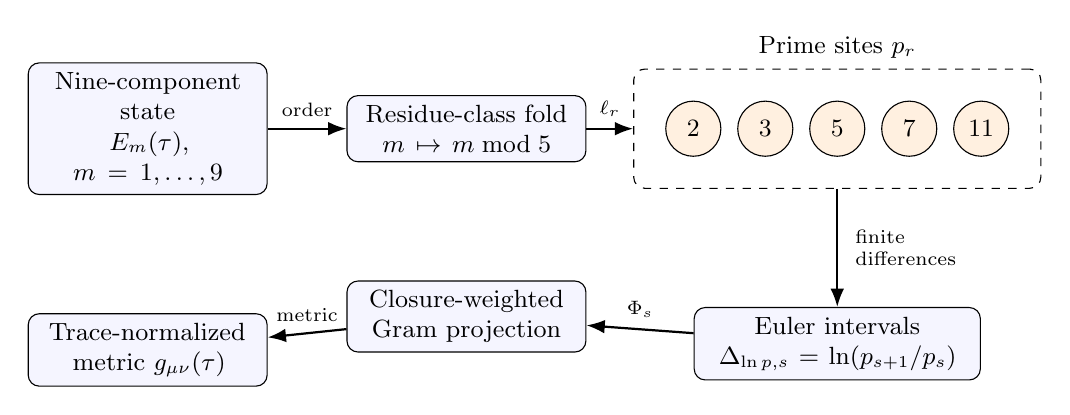
\begin{tikzpicture}[
  >=Latex,
  flow/.style={draw,rounded corners,align=center,minimum height=8mm,
               text width=28mm,fill=blue!4},
  prime/.style={circle,draw,minimum size=7mm,fill=orange!12,inner sep=0pt},
  every node/.style={font=\small}
]
\node[flow] (state) {Nine-component state\\$E_m(\tau)$, $m=1,\ldots,9$};
\node[flow,right=10mm of state] (fold) {Residue-class fold\\$m\mapsto m\bmod 5$};
\node[prime,right=10mm of fold] (p2) {$2$};
\node[prime,right=2mm of p2] (p3) {$3$};
\node[prime,right=2mm of p3] (p5) {$5$};
\node[prime,right=2mm of p5] (p7) {$7$};
\node[prime,right=2mm of p7] (p11) {$11$};
\node[draw,dashed,rounded corners,fit=(p2)(p3)(p5)(p7)(p11),
      inner sep=4mm,label=above:{Prime sites $p_r$}] (primebox) {};

\node[flow,below=15mm of state] (metric) {Trace-normalized\\metric $g_{\mu\nu}(\tau)$};
\node[flow,below=15mm of fold] (gram) {Closure-weighted\\Gram projection};
\node[flow,text width=34mm,below=15mm of primebox] (euler)
  {Euler intervals\\$\Delta_{\ln p,s}=\ln(p_{s+1}/p_s)$};

\draw[->,thick] (state) --
  node[midway,above=1mm,font=\scriptsize,fill=white,inner sep=1pt]{order} (fold);
\draw[->,thick] (fold) --
  node[midway,above=1mm,font=\scriptsize,fill=white,inner sep=1pt]{$\ell_r$} (primebox);
\draw[->,thick] (primebox.south) --
  node[midway,right=1mm,font=\scriptsize,align=left]{finite\\differences} (euler.north);
\draw[->,thick] (euler) --
  node[midway,above=1mm,font=\scriptsize,fill=white,inner sep=1pt]{$\Phi_s$} (gram);
\draw[->,thick] (gram) --
  node[midway,above=1mm,font=\scriptsize,fill=white,inner sep=1pt]{metric} (metric);
\end{tikzpicture}
\caption{Prime-lattice RG folding.  The ordered nine-component entropy state
is folded by residue class onto the five prime sites; finite differences over
the four logarithmic Euler intervals feed the closure-weighted Gram projection.}
\label{fig:prime-lattice-rg-folding}
\end{figure}

Its logarithms are the radial RG coordinates,
\begin{equation}
\label{eq:section-five-log-prime-coordinate}
 x_r=\bigl(\ln p_r\bigr),
 \qquad
 r=0,
\ldots,4,
\end{equation}
so nearest-neighbor finite differences on this lattice are naturally divided by
$\ln(p_{s+1}/p_s)=x_{s+1}-x_s$.  The role of the prime basis is not to introduce
a new spectrum of particles.  It is a fixed, finite coordinate frame in which
the ordered boundary entropy state can be compressed into four Euler intervals
and then lifted to a symmetric metric tensor.

Let
\begin{equation}
\label{eq:section-five-dominant-sequence-reminder}
 \sigma=(c_1,\ldots,c_9)
\end{equation}
be the dominant loading sequence of
Eq.~\eqref{eq:section-four-dominant-loading-sequence}.  The partially resolved
entanglement state at RG parameter $\tau$ is the interpolation of the discrete
self-resolution records,
\begin{equation}
\label{eq:section-five-interpolated-entropy-state}
 \Omega_{\tau}(c)
 =
 \sum_{n=1}^{9}
 \theta_n(\tau)\,
 \delta_{c_n,c}\,
 \Delta T_n,
\end{equation}
where
\begin{equation}
\label{eq:section-five-resolution-window}
 \theta_n(\tau)
 =
 \begin{cases}
 0,& \tau<\tau_{n-1},\\
 \dfrac{\tau-\tau_{n-1}}{\tau_n-\tau_{n-1}},&
 \tau_{n-1}\le\tau\le\tau_n,\\
 1,& \tau>\tau_n.
 \end{cases}
\end{equation}
Consequently $\sum_{c\in\mathcal C}\Omega_{\tau}(c)=\tau$.  The metric
projector uses both the static entanglement density and the resolved entropy
state.  Along the ordered sequence define
\begin{equation}
\label{eq:section-five-sequence-entanglement-mass}
 E_m(\tau)
 =
 \rho_E(c_m)+\Omega_{\tau}(c_m),
 \qquad
 m=1,\ldots,9.
\end{equation}
Since $\sum_{m=1}^9\rho_E(c_m)=1$ and
$\sum_{m=1}^9\Omega_{\tau}(c_m)=\tau$, the total resolved load before folding
is
\begin{equation}
\label{eq:section-five-total-sequence-load}
 \sum_{m=1}^{9}E_m(\tau)=1+\tau.
\end{equation}
The five-component load vector is obtained by folding this ordered sequence
onto the prime lattice by residue class,
\begin{align}
\label{eq:section-five-load-vector-construction}
 \widehat\ell_r(\tau)
 &=
 \sum_{m=1}^{9}
 E_m(\tau)\,
 \mathbf 1_{\{m-1\equiv r\;(\bmod\;5)\}},
 \qquad r=0,\ldots,4,\nonumber\\
 \ell_r(\tau)
 &=
 \frac{\widehat\ell_r(\tau)}
 {\sum_{q=0}^{4}\widehat\ell_q(\tau)}
 =
 \frac{\widehat\ell_r(\tau)}{1+\tau}.
\end{align}
This gives
\begin{equation}
\label{eq:section-five-load-vector-normalization}
 \ell_r(\tau)>0,
 \qquad
 \sum_{r=0}^{4}\ell_r(\tau)=1.
\end{equation}
The dependence on $\sigma$ is essential: the same multiset of boundary
entropies would give a different prime-lattice load only if the modular loading
order were changed.  Equal-density ties retain the fixed lexicographic convention
already specified in Section~\ref{sec:boundary-entropy-densities-self-resolution}.

The Euler flux is the logarithmic finite difference of the load vector across
adjacent prime sites.  For $s=0,1,2,3$,
\begin{equation}
\label{eq:section-five-euler-flux}
 \Phi_s(\tau)
 =
 \frac{\ell_{s+1}(\tau)-\ell_s(\tau)}
 {\ln(p_{s+1}/p_s)}.
\end{equation}
Thus $\Phi_s$ is the discrete RG gradient
$\Delta\ell/\Delta\ln p$ on the finite prime lattice.  The local mean loading
and arithmetic hardness factor are
\begin{equation}
\label{eq:section-five-mean-loading-hardness}
 \bar\ell_s(\tau)
 =
 \frac{\ell_s(\tau)+\ell_{s+1}(\tau)}{2},
 \qquad
 h_s=\frac{1}{p_s}+\frac{1}{p_{s+1}}.
\end{equation}
The closure-weighted contribution of the $s$th Euler interval is
\begin{equation}
\label{eq:section-five-weight-functions}
 W_s(\tau)
 =
 \lambda_{\text{closure}}
 \bigl(|\Phi_s(\tau)|+\bar\ell_s(\tau)+h_s\bigr),
 \qquad
 \lambda_{\text{closure}}>0.
\end{equation}
Every term in Eq.~\eqref{eq:section-five-weight-functions} is nonnegative, so
the outer-product part of the metric projection is positive semidefinite.  The
absolute flux measures local entropy shear, the mean load measures local
occupancy, and $h_s$ prevents a completely flat load vector from erasing the
arithmetic interval.

The four Euler embedding vectors place the four intervals into the static
metric block.  Let $e_s^{\mu}=\delta_s^{\mu}$ for
$\mu,s=0,1,2,3$, and read all load-vector indices modulo $5$.  The embedding
vector is
\begin{equation}
\label{eq:section-five-execution-vectors}
 v_s^{\mu}(\tau)
 =
 e_s^{\mu}
 +
 \left(
 \ell_s+\delta_{s0},
 \ell_{s+1}+\delta_{s1},
 \ell_{(s+2)\,(\bmod\,5)}+\delta_{s2},
 |\Phi_s|+\ell_{(s+3)\,(\bmod\,5)}+\delta_{s3}
 \right)^{\mu}.
\end{equation}
The Kronecker terms mark the Euler interval, while the cyclic load entries
couple each interval to the neighboring prime sites.  The fourth component also
contains $|\Phi_s|$, so entropy shear enters the block as a metric direction
rather than only as a scalar weight.

The unstabilized static metric is the weighted Gram matrix of these execution
vectors, plus a positive diagonal closure floor,
\begin{equation}
\label{eq:section-five-unstabilized-metric}
 \widetilde g_{\mu\nu}(\tau)
 =
 \sum_{s=0}^{3}
 W_s(\tau)\,v_{s\mu}(\tau)v_{s\nu}(\tau)
 +
 \diag(d_0,d_1,d_2,d_3)_{\mu\nu}.
\end{equation}
The diagonal entries are
\begin{equation}
\label{eq:section-five-diagonal-floor}
 d_s(\tau)
 =
 \lambda_{\text{closure}}+W_s(\tau)+\ell_s(\tau)+\ell_{s+1}(\tau),
 \qquad
 s=0,1,2,3.
\end{equation}
Since $\lambda_{\text{closure}}>0$ and the remaining terms are nonnegative,
Eq.~\eqref{eq:section-five-diagonal-floor} gives a strictly positive diagonal
regularizer.  The tensor in Eq.~\eqref{eq:section-five-unstabilized-metric} is
therefore already a finite, positive candidate for the static block; the final
step enforces exact symmetry and trace normalization in the same way for every
slice.

Define
\begin{equation}
\label{eq:section-five-symmetrized-lifted-block}
 A_{\mu\nu}(\tau)
 =
 \operatorname{Sym}
 \bigl(
 \widetilde g_{\mu\nu}(\tau)+\epsilon_{\text{eig}}\delta_{\mu\nu}
 \bigr),
 \qquad
 \operatorname{Sym}(B)_{\mu\nu}
 =
 \frac{B_{\mu\nu}+B_{\nu\mu}}{2}.
\end{equation}
The eigenvalue lift is chosen as
\begin{equation}
\label{eq:section-five-eigenvalue-lift}
 \epsilon_{\text{eig}}
 =
 \max\!\bigl(0,\epsilon_{\text{pos}}
 -\lambda_{\min}(\operatorname{Sym}\widetilde g)\bigr),
 \qquad
 \epsilon_{\text{pos}}>0.
\end{equation}
In exact arithmetic the positive diagonal floor usually makes the lift
unnecessary, but the construction retains Eq.~\eqref{eq:section-five-eigenvalue-lift} so
that numerical roundoff cannot produce a nonpositive metric slice.  The
physical static metric is
\begin{equation}
\label{eq:section-five-stabilized-trace-normalized-metric}
 \boxed{
 g_{\mu\nu}(\tau)
 =
 \frac{A_{\mu\nu}(\tau)}{\Tr A(\tau)}
 =
 \frac{
 \operatorname{Sym}
 \bigl(\widetilde g_{\mu\nu}(\tau)+\epsilon_{\text{eig}}\delta_{\mu\nu}\bigr)}
 {\Tr\!\bigl[
 \operatorname{Sym}\widetilde g(\tau)
 +\epsilon_{\text{eig}}\mathbf{1}_4\big]}.
 }
\end{equation}
It obeys the metric-slice checks
\begin{equation}
\label{eq:section-five-metric-checks}
 g_{\mu\nu}=g_{\nu\mu},
 \qquad
 \Tr g=1,
 \qquad
 \lambda_{\min}(g)>0.
\end{equation}
The trace condition fixes the finite-register scale of the slice; it does not
remove physical anisotropy, because anisotropy is carried by the normalized
eigenvalue ratios and off-diagonal components inherited from the execution
vectors.

The spatial bulk metric is the projection of the static $4\times4$ block onto
the three rendered spatial directions.  With
\begin{equation}
\label{eq:section-five-static-to-bulk-projector}
 P_a{}^{\mu}
 =
 \begin{pmatrix}
 0&1&0&0\\
 0&0&1&0\\
 0&0&0&1
 \end{pmatrix},
 \qquad
 a=1,2,3,
 \qquad
 \mu=0,1,2,3,
\end{equation}
the induced spatial metric is
\begin{equation}
\label{eq:section-five-spatial-bulk-metric}
 g_{ab}^{\text{bulk}}(\tau)
 =
 P_a{}^{\mu}
 g_{\mu\nu}^{\text{static}}(\tau)
 P_b{}^{\nu}.
\end{equation}
Equivalently, the spatial block is the lower-right $3\times3$ principal block
of the stabilized static metric in this benchmark projector.  Other projectors
could rotate the rendered spatial frame, but the canonical projection uses the fixed matrix in
Eq.~\eqref{eq:section-five-static-to-bulk-projector} so that the benchmark is
deterministic.

Combining the construction gives the complete holographic RG map
\begin{equation}
\label{eq:section-five-complete-rg-map}
 \boxed{
 \nabla_{\mathcal C}S_{\partial}
 \longmapsto
 \rho_E(i,j)
 \longmapsto
 \ell_r(\tau)
 \longmapsto
 \Phi_s(\tau),W_s(\tau),v_s^{\mu}(\tau)
 \longmapsto
 g_{\mu\nu}(\tau)
 \longmapsto
 g_{ab}^{\text{bulk}}(\tau)
 }.
\end{equation}
The shortened form is
\begin{equation}
\label{eq:section-five-short-rg-map}
 \nabla_{\mathcal C}S_{\partial}
 \longrightarrow
 \rho_E(i,j)
 \longrightarrow
 \ell_r(\tau)
 \longrightarrow
 g_{\mu\nu}(\tau).
\end{equation}
Every arrow is fixed by the previous sections: the boundary entropy gradient
comes from modular-overlap loading, $\rho_E$ is the normalized entanglement
density, $\ell_r$ is the prime-lattice compression of the ordered resolved
state, and $g_{\mu\nu}$ is the stabilized trace-one Gram projection.  No
independent bulk equation of motion is inserted between the boundary entropy
state and the static metric slice.

This is the precise deviation from standard holographic RG.  The usual
AdS/CFT construction treats the bulk metric as a dynamical saddle governed by
the Einstein--Hilbert action; the boundary scale dependence is recovered by
solving radial Hamilton--Jacobi flow equations.  SHBT instead uses the closed
finite boundary register as the primitive object.  The replacement is
\begin{equation}
\label{eq:section-five-standard-to-shbt-rg-replacement}
 \left(
 S(A),\rho,S_{\text{os}}
 \right)_{\text{standard}}
 \longrightarrow
 \left(
 \rho_B,\rho_E,\Omega_{\tau},x_r=\ln p_r
 \right)_{\text{SHBT}},
 \qquad
 \partial_{\rho}
 \longrightarrow
 \Delta_{\ln p}.
\end{equation}
Thus Eq.~\eqref{eq:section-five-standard-hj-flow} is not solved as an
independent bulk field equation.  Its SHBT analogue is the finite algebraic
pipeline
\begin{equation}
\label{eq:section-five-shbt-rg-comparison-map}
 (\rho_B,\rho_E,\Omega_{\tau})
 \longmapsto
 \ell_r(\tau)
 \longmapsto
 \Phi_s(\tau)
 \longmapsto
 \widetilde g_{\mu\nu}(\tau)
 \longmapsto
 g_{\mu\nu}(\tau),
\end{equation}
with closure, positivity, and trace normalization checked slice by slice.

\begin{center}
\small
\begin{tabular}{@{}L{0.30\linewidth}L{0.30\linewidth}L{0.30\linewidth}@{}}
\toprule
Feature & Standard holographic RG & SHBT RG flow \\
\midrule
Primitive data & Continuum boundary QFT and classical bulk saddle &
Completed finite boundary CFT and modular-overlap densities \\
Radial scale & Continuous $\rho$ or $z$, with $\mu\propto e^{\rho/L}\propto z^{-1}$ &
Discrete prime sites $x_r=\ln p_r$ and Euler intervals $\Delta_{\ln p}$ \\
Entanglement role & RT surfaces measure entropy from a given bulk metric &
Normalized entropy densities synthesize the metric slice \\
Dynamics & Einstein--Hilbert equations recast as Hamilton--Jacobi flow &
Deterministic entropy self-resolution and weighted Gram projection \\
Deviation & Large-$N$ semiclassical bulk is assumed &
No independent bulk dynamics is assumed; geometry is a closed projection \\
\bottomrule
\end{tabular}
\end{center}

The physical closure map for this section is
\begin{center}
\small
\begin{tabular}{@{}L{0.38\linewidth}L{0.54\linewidth}@{}}
\toprule
Physical object & Mathematical definition or closure condition \\
\midrule
Resolved entropy load & $\rho_E,\sigma,\Omega_{\tau}\mapsto\ell_r$ \\
Discrete RG flux & $\Phi_s=\Delta\ell/\Delta\ln p$ \\
Static metric synthesis & $\ell_r\mapsto\Phi_s,W_s,v_s^{\mu},g_{\mu\nu}$ \\
Spatial bulk projection & $P_a{}^{\mu}g_{\mu\nu}P_b{}^{\nu}$ \\
Metric closure & Symmetry, unit trace, and positive eigenvalues \\
Slice data & $\ell_r$, $\Phi_s$, $g_{\mu\nu}$, $\gamma_{ab}$, and their spectra \\
\bottomrule
\end{tabular}
\end{center}
The load construction in Eq.~\eqref{eq:section-five-load-vector-construction},
the metric synthesis in
Eqs.~\eqref{eq:section-five-euler-flux}--\eqref{eq:section-five-stabilized-trace-normalized-metric},
and the spatial projection in Eq.~\eqref{eq:section-five-spatial-bulk-metric}
therefore form a single mathematical map.  Its output is admissible only when
Eq.~\eqref{eq:section-five-metric-checks} holds, the spatial block has dimension
$3\times3$, the slice order agrees with the dominant loading sequence, and no
negative eigenvalue remains after stabilization.

\section{Topological Baryogenesis and Anti-Baryon State Decoupling}
\label{sec:topological-baryogenesis-anti-baryon-state-decoupling}

The baryogenesis sector uses the completed boundary branch to separate two
questions that are usually entangled.  The first is the size of the visible
baryon excess.  The second is the fate of the anti-baryon stress-energy that
would ordinarily accompany visible anti-baryon charge.  The visible excess is
fixed by a topological CP invariant and a modular restoration scale.  The
stress-energy is treated by an active Stinespring isometric state-projection map
that strips visible color and electromagnetic charge while preserving the passive gravitational source.  The
mechanism is therefore not a dynamical erasure of stress-energy.  It is a
projection of active render channels into the dark completion sector, constrained
by the same framing closure that fixes the branch.

The visible electroweak conversion factor is the standard sphaleron coefficient
for the rendered Standard Model channel,
\begin{equation}
\label{eq:section-six-sphaleron-coefficient}
 C_{\text{sph}}
 =
 \frac{28}{79}.
\end{equation}
This coefficient converts the topological lepton-sector seed into the baryon
number observed in the active visible register.  In SHBT the CP-odd seed is not
introduced as a free phase.  It is the level-locked topological Jarlskog
invariant
\begin{equation}
\label{eq:section-six-topological-jarlskog}
 \boxed{
 J_{\text{CP}}^{\text{topo}}
 =
 \frac{1}{\Kpar}
 \left(\frac{\kq}{\kell+2}\right)
 \sqrt{1-\kappad^{2}}
 \sin\!\left(\frac{2\pi\kq}{\kell}\right).
 }
\end{equation}
The factors have distinct origins.  The parent completion contributes the
dilution $1/\Kpar$; the visible level mismatch contributes
$\kq/(\kell+2)$, with the $+2$ the $SU(2)$ dual-Coxeter shift; the dark
completion contributes the admissible overlap factor
$\sqrt{1-\kappad^{2}}$; and the modular phase difference between the quark
and lepton clocks contributes $\sin(2\pi\kq/\kell)$.  Thus CP violation is a
residue of completed modular transport rather than an independently tunable
angle.

The heavy restoration scale is fixed by the same branch arithmetic.  Define the
rank projection factor by
\begin{equation}
\label{eq:section-six-rank-projection-factor}
 \Pi_{\text{rank}}
 =
 \sqrt{
 \frac{(h^{\vee}_{SO(10)}\dimop SO(10))/12}
 {(h^{\vee}_{SU(3)}\dimop SU(3))/12}}
 \sqrt{\frac{\kq+h^{\vee}_{SU(3)}}{\Kpar+h^{\vee}_{SO(10)}}}.
\end{equation}
The residual matching of the $126$ completion channel is written
$\delta\Pi_{126}^{\text{match}}$.  The modular restoration mass is then
\begin{equation}
\label{eq:section-six-modular-restoration-scale}
 \boxed{
 M_N
 =
 M_{\text{GUT}}
 \exp\!\left[-\left(
 I_{\ell}^{\star}\Pi_{\text{rank}}
 +
 I_q^{\star}\delta\Pi_{126}^{\text{match}}
 \right)\right].
 }
\end{equation}
For the canonical branch $I_{\ell}^{\star}=6$ and $I_q^{\star}=13$, so the
exponent is a structural suppression determined by the completed embedding.  It
is not adjusted after the baryon asymmetry is computed.

The topological baryogenesis identity derived below is therefore a consistency
check of the completed modular transport: the same algebra that fixes the
visible levels and the dark completion residue also fixes the CP-odd seed and
the restoration scale.  The numerical outcome \(\eta_B\approx6.45\times10^{-10}\)
is not a free parameter introduced to match observations; it is the residue of
the modular phase mismatch between the quark and lepton clocks after the center
lifts are locked.  Thus the benchmark calculation reported in
Section~\ref{sec:numerical-verification-performance} is a verification that the
branch arithmetic reproduces the observed visible asymmetry, but it does not
claim to be an independent, unconstrained prediction of the baryon abundance
without the branch data.

The SHBT baryogenesis identity is therefore
\begin{equation}
\label{eq:section-six-baryon-asymmetry}
 \boxed{
 \eta_B
 =
 C_{\text{sph}}\,J_{\text{CP}}^{\text{topo}}\,\frac{M_N}{\MP}.
 }
\end{equation}
The four ingredients in Eq.~\eqref{eq:section-six-baryon-asymmetry} are fixed
by the electroweak conversion coefficient, the modular CP residue, the
restoration scale, and the Planck normalization.  Substitution of the canonical
branch data gives \(\eta_B=6.449923359416\times10^{-10}\).

The visible asymmetry becomes a complete accounting statement only after the
anti-baryon channel is specified.  Let $\mathcal H_{\bar B}^{\text{vis}}$ denote
the active visible anti-baryon Hilbert space.  For a visible anti-baryon density
matrix $\rho$, define the active render cost
\begin{equation}
\label{eq:section-six-active-render-cost}
 \boxed{
 \mathcal C_{\bar B}(\rho)
 =
 \gamma_3\Tr(\rho Q_{SU(3)}^2)
 +
 \gamma_{\text{EM}}\Tr(\rho Q_{\text{EM}}^2)
 +
 \gamma_{\text{fr}}\Deltafr^2,
 \qquad
 \gamma_3,\gamma_{\text{EM}},\gamma_{\text{fr}}>0.
 }
\end{equation}
This is an active rendering functional, not a passive mass functional.  It
counts the cost of keeping anti-baryons visible as colored and electrically
charged excitations, plus any residual framing mismatch.  On the canonical
branch $\Deltafr=0$, so the only nonzero active cost comes from visible gauge
charge.

The Stinespring isometric state-projection operator is the completion-sector projection
\begin{equation}
\label{eq:section-six-state-projection-operator}
 \mathcal D_{\bar B}:
 \mathcal H_{\bar B}^{\text{vis}}
 \longrightarrow
 \mathcal H_{\text{dark}}^{\text{B-L}},
 \qquad
 \rho_{\bar B}^{(n+1)}
 =
 \frac{
 \mathcal D_{\bar B}\rho_{\bar B}^{(n)}\mathcal D_{\bar B}^{\dagger}}
 {\Tr\!\left(
 \mathcal D_{\bar B}\rho_{\bar B}^{(n)}\mathcal D_{\bar B}^{\dagger}
 \right)}.
\end{equation}
The Stinespring isometric state-projection map $\mathcal D_{\bar B}$ acts at the modular restoration
scale $M_N$ given in
Eq.~\eqref{eq:section-six-modular-restoration-scale}.  This scale is
determined by the same branch arithmetic that fixes the parent completion and
the framing defect.  In the boundary theory, the transition is a continuous,
unitary projection in the completed Hilbert space: as the energy scale descends
from the GUT scale toward $M_N$, the visible anti-baryon gauge currents lose
their support on the active $SU(3)$ and $U(1)_{\text{EM}}$ channels.  Equivalently,
the projection is a constant phase-transition boundary condition in the
register: the active render cost $\mathcal C_{\bar B}$ drops to zero exactly at
the scale where the modular restoration exponent vanishes.  For any finite
Causal Point, however, this state decoupling is only observed as a local
horizon-conditioned effect: if the observer's horizon fraction $f_H$
(Eq.~\eqref{eq:section-seven-local-horizon-fraction}) is too small, the active
visible anti-baryon channels are already below the local entropy resolution
limit, so the state decoupling appears to the local observer as a pre-existing
completion asymmetry rather than a dynamical phase transition.  Thus the
mechanism has two complementary descriptions: (i) a bulk phase transition at
$M_N$ in the completed boundary data, and (ii) an observer-conditional
projection for any Causal Point with $f_H$ below the threshold required to
resolve active anti-baryon gauge charges.  The canonical branch fixes $M_N$
once; the observer dependence only determines whether the local history record
includes the transition, not whether the dark completion sector stores the
passive stress-energy.

It is defined by the active charge-stripping constraints
\begin{equation}
\label{eq:section-six-stripping-constraints}
 \boxed{
 \mathcal D_{\bar B}^{\dagger}Q_{SU(3)}\mathcal D_{\bar B}=0,
 \qquad
 \mathcal D_{\bar B}^{\dagger}Q_{\text{EM}}\mathcal D_{\bar B}=0.
 }
\end{equation}
The dark target stores the conjugate $B-L$ residue, so the completed boundary
state remains neutral even though the active visible anti-baryon gauge channels
are no longer rendered.

Stress-energy preservation is imposed on the passive source, not on the active
charge cost.  The defining equality is
\begin{equation}
\label{eq:section-six-stress-energy-preservation}
 \boxed{
 \Tr\!\left(\rho^{(n)}T_{\mu\nu}^{\bar B,\text{passive}}\right)
 =
 \Tr\!\left(\rho^{(n+1)}T_{\mu\nu}^{\text{dark},\text{passive}}\right).
 }
\end{equation}
Thus the visible register can lose active anti-baryon color and electromagnetic
support without violating the gravitational accounting used by the topological
Einstein equation.  Equivalently, the decoupled anti-baryon contributes as a
dark passive source rather than as an actively rendered visible particle.

The anti-baryon loop closes at the fixed point
\begin{equation}
\label{eq:section-six-antibaryon-fixed-point}
 \boxed{
 \rho_{\bar B}^{\star}
 =
 \frac{
 \mathcal D_{\bar B}\rho_{\bar B}^{\star}\mathcal D_{\bar B}^{\dagger}}
 {\Tr\!\left(
 \mathcal D_{\bar B}\rho_{\bar B}^{\star}\mathcal D_{\bar B}^{\dagger}
 \right)},
 \qquad
 \mathcal C_{\bar B}(\rho_{\bar B}^{\star})=0,
 \qquad
 \delta T_{\mu\nu}^{\text{passive}}=0.
 }
\end{equation}
At this point the anti-baryon is absent from the active visible gauge-rendered
channels, while its passive stress-energy has been moved into the dark
completion sector.  The observed baryon asymmetry is therefore a render-channel
asymmetry, not an unbalanced disappearance of energy-momentum.

The physical closure conditions for this section are
\begin{center}
\small
\begin{tabular}{@{}L{0.38\linewidth}L{0.54\linewidth}@{}}
\toprule
Physical operator or observable & Mathematical definition or closure condition \\
\midrule
Baryon asymmetry & $\eta_B=C_{\text{sph}}J_{\text{CP}}^{\text{topo}}M_N/\MP$ \\
Active render cost & $\mathcal C_{\bar B}(\rho)$ in Eq.~\eqref{eq:section-six-active-render-cost} \\
Charge-decoupling map & $\mathcal D_{\bar B}^{\dagger}Q_{SU(3)}\mathcal D_{\bar B}=\mathcal D_{\bar B}^{\dagger}Q_{\text{EM}}\mathcal D_{\bar B}=0$ \\
Passive source equality & Eq.~\eqref{eq:section-six-stress-energy-preservation} \\
Fixed-point state & $\rho_{\bar B}^{\star}$ with $\mathcal C_{\bar B}=0$ \\
Completed accounting & $\delta T_{\mu\nu}^{\text{passive}}=0$ \\
\bottomrule
\end{tabular}
\end{center}
Together these conditions distinguish the active gauge-rendering functional
from the passive gravitational source.  The former vanishes at the projected
fixed point, while the latter is exactly transferred to the dark completion
sector.  Implementation identifiers and performance diagnostics for this map
are isolated in Section~\ref{sec:code-availability}.

\section{Causal Point and History Crystallization}
\label{sec:causal-point-history-crystallization}

The Causal Point is the observer interface of SHBT.  It is not an external
classical system appended to the boundary theory, but a finite local address
inside the completed register.  Its job is to translate global holographic
closure into the quantities an observer can actually sample: a local memory
budget, a local valuation of hidden information, a past-light-cone loading
flow, and a deterministic projection that crystallizes one history from a
finite outcome ensemble.  Thus observation is treated as an entropy-budgeted
operation on the boundary register rather than as a primitive background
process.

The global horizon follows directly from the saturated bit budget introduced in
the Introduction.  Since $\Nbits=3\pi/(\Lp^2\Lholo)$, the horizon radius is
\begin{equation}
\label{eq:section-seven-global-horizon}
 \boxed{
 R_H
 =
 \sqrt{\frac{\Nbits\Lp^2}{\pi}}
 =
 \sqrt{\frac{3}{\Lholo}}.
 }
\end{equation}
For a Causal Point whose local sampling radius is $R_{\text{local}}$, define the
horizon fraction and local area by
\begin{equation}
\label{eq:section-seven-local-horizon-fraction}
 f_H
 =
 \frac{R_{\text{local}}}{R_H},
 \qquad
 A_{\text{local}}=4\pi R_{\text{local}}^2,
 \qquad
 0\le f_H\le1.
\end{equation}
The observer cannot address the full horizon register unless $f_H=1$.  The
available local memory, hidden complement, and operational entropy limit are
therefore
\begin{equation}
\label{eq:section-seven-local-memory-budget}
 \boxed{
 N_{\text{local}}
 =
 \Nbits f_H^2,
 \qquad
 N_{\text{hidden}}
 =
 \Nbits-N_{\text{local}},
 \qquad
 N_{\text{limit}}
 =
 \min\!\left(
 N_{\text{local}},
 \frac{A_{\text{local}}}{4\Lp^2\ln2}
 \right).
 }
\end{equation}
The first entry counts addressable register bits.  The second counts degrees of
freedom outside the local addressable patch.  The third enforces the stricter
of the local register count and the local area-law bound, with the factor
$\ln2$ converting the area entropy into bits.

The Causal Point's self-valuation is the scalar response of the local observer
to residual framing and hidden-sector loading.  Writing
$\Delta_{\text{frame}}\equiv\Deltafr$ and
\begin{equation}
\label{eq:section-seven-hidden-fraction}
 f_{\text{hidden}}
 =
 \frac{N_{\text{hidden}}}{\Nbits}
 =
 1-\frac{N_{\text{local}}}{\Nbits},
 \qquad
 w(\xi)=\frac{\xi_{\ell}+\xi_q+\xi_s}{3},
\end{equation}
the valuation field is
\begin{equation}
\label{eq:section-seven-self-valuation}
 \boxed{
 \Sigma
 =
 (1+\Delta_{\text{frame}})
 \bigl(1+w(\xi)f_{\text{hidden}}\bigr).
 }
\end{equation}
On the canonical branch $\Delta_{\text{frame}}=0$, but the formula is written in a
branch-independent form so that any residual framing mismatch would be visible
as a multiplicative observer cost.  The localized entropy gradient is the
valuation density across the local sampling radius,
\begin{equation}
\label{eq:section-seven-localized-entropy-gradient}
 \boxed{
 \nabla_{\text{obs}}\Sigma
 =
 \frac{\Sigma f_{\text{hidden}}}{R_{\text{local}}}.
 }
\end{equation}
The apparent observer acceleration is then
\begin{equation}
\label{eq:section-seven-apparent-acceleration}
 \boxed{
 a_{\text{obs}}
 =
 c^2\nabla_{\text{obs}}\Sigma.
 }
\end{equation}
This acceleration is not inserted as an external force law.  It is the local
inertial response to the hidden entropy gradient seen by an entropy-limited
observer.

The same local data define the observer-frame Jacobian.  The anisotropy
coordinates $(\xi_{\ell},\xi_q,\xi_s)$ are the three directional entries stored
in the local property packet, and the Causal Point projection matrix is
\begin{equation}
\label{eq:section-seven-observer-jacobian}
 \boxed{
 J^{\mu}{}_{\nu}
 =
 \begin{pmatrix}
 1 + \Sigma f_{\text{hidden}} & -\Sigma\xi_{\ell} & -\Sigma\xi_q & -\Sigma\xi_s\\
 0 & 1+\Sigma\xi_{\ell} & 0 & 0\\
 0 & 0 & 1+\Sigma\xi_q & 0\\
 0 & 0 & 0 & 1+\Sigma\xi_s
 \end{pmatrix}.
 }
\end{equation}
Applied to a bulk metric slice from Section~\ref{sec:holographic-rg-flow-boundary-entropy-bulk-metric},
it gives the observer-frame metric
\begin{equation}
\label{eq:section-seven-observer-metric-pullback}
 g^{\text{obs}}_{\mu\nu}
 =
 J_{\mu}{}^{\alpha}g_{\alpha\beta}J_{\nu}{}^{\beta}.
\end{equation}
The off-diagonal entries in the first row encode the finite-register mixing
between temporal sampling and the three anisotropic property channels, while
the diagonal spatial entries encode direction-dependent local rescaling.

Past-light-cone flow is the observer-time image of a static boundary loading
process.  Let $N_{\text{load}}(t)$ be the number of loaded bits along the sampled
history.  The loading fraction and effective expansion rate are
\begin{equation}
\label{eq:section-seven-loading-law}
 \boxed{
 f_{\text{load}}(t)
 =
 \frac{N_{\text{load}}(t)}{\Nbits},
 \qquad
 H_{\text{eff}}(t)
 =
 H_{\Lambda}+\frac{1}{3}\frac{df_{\text{load}}}{dt}.
 }
\end{equation}
Here $H_{\Lambda}$ is the horizon rate associated with the static
$\Lholo$ sector.  The second term is not a new external clock; it is the
one-dimensional residue of finite boundary loading as reconstructed by the
Causal Point.  Along the observer's past light cone, redshift parameterizes the
same process through
\begin{equation}
\label{eq:section-seven-past-light-cone-flow}
 \boxed{
 \frac{dt}{dz}
 =
 -\frac{1}{(1+z)H_{\text{eff}}(z)},
 \qquad
 \frac{d\chi}{dz}
 =
 \frac{1}{H_{\text{eff}}(z)}.
 }
\end{equation}
The first equation gives the lookback-time increment, and the second gives the
comoving radial increment in the same light-cone units.  A sampled redshift
therefore selects a boundary coordinate by the ordered loading sequence,
\begin{equation}
\label{eq:section-seven-coordinate-flow}
 n(z)
 =
 1+
 \left\lfloor\bigl(|\sigma|-1\bigr)f_{\text{load}}(z)\right\rfloor,
 \qquad
 c(z)=\sigma_{n(z)}\in\mathcal C.
\end{equation}
This gives the bridge between the apparent cosmological flow and the finite
boundary address on which a measurement can be attempted.

History crystallization begins only after such a boundary address has been
selected.  Let $\mathcal R$ be the finite register visible to the Causal Point,
let $A\in\mathcal R$ be the selected address, and let
\begin{equation}
\label{eq:section-seven-outcome-ensemble}
 \Omega_A
 =
 \{\omega_0,\omega_1,\ldots,\omega_{m-1}\},
 \qquad
 \sum_{i=0}^{m-1}p_i=1,
 \qquad
 p_i\ge0,
\end{equation}
be the finite outcome ensemble and its normalized local loading weights.  The
entropy costs of a retrieval event are
\begin{align}
\label{eq:section-seven-retrieval-costs}
 C_{\text{addr}}
 &=
 \log_2|\mathcal R|,
 &
 C_{\text{ens}}
 &=
 \log_2|\Omega_A|,\notag\\
 C_{\text{get}}
 &=
 \max\!\left(1,C_{\text{addr}}+C_{\text{ens}},C_{\text{req}}\right),
 &
 R_{\text{entropy}}
 &=
 N_{\text{limit}}-C_{\text{get}}.
\end{align}
The GET operation is admissible exactly when
\begin{equation}
\label{eq:section-seven-retrieval-admissibility}
 R_{\text{entropy}}\ge0.
\end{equation}
If the residual is negative, the Causal Point has insufficient local entropy
budget to crystallize the requested classical record.

When the budget condition holds, the deterministic collapse index is
\begin{equation}
\label{eq:section-seven-collapse-index}
 \boxed{
 \iota
 =
 \operatorname{Hash}\!\left(
 \mathcal O,
 A,
 f_H,
 N_{\text{local}},
 m
 \right)
 \bmod m.
 }
\end{equation}
The corresponding rank-one projection operator is
\begin{equation}
\label{eq:section-seven-history-projection}
 \boxed{
 \Pi_{A,\iota}
 =
 |A,\omega_{\iota}\rangle\langle A,\omega_{\iota}|.
 }
\end{equation}
For a sequence of admissible Causal Point retrievals, the history density matrix
updates by
\begin{equation}
\label{eq:section-seven-history-update}
 \rho_{\text{hist}}^{(n+1)}
 =
 \frac{
 \Pi_{A_n,\iota_n}\rho_{\text{hist}}^{(n)}\Pi_{A_n,\iota_n}}
 {\Tr\!\left(
 \Pi_{A_n,\iota_n}\rho_{\text{hist}}^{(n)}
 \right)}.
\end{equation}
The full crystallized history along a sampled past light cone is therefore the
ordered product
\begin{equation}
\label{eq:section-seven-full-history-projector}
 \begin{aligned}
 \Pi_{\text{history}}(z_1,\dots,z_m)
 &=
 \Pi_{A_m,\iota_m}\cdots\Pi_{A_2,\iota_2}\Pi_{A_1,\iota_1},\\
 A_n&=A\bigl(c(z_n)\bigr).
 \end{aligned}
\end{equation}
Thus a classical past is not retrieved from an unlimited archive.  It is the
finite ordered record that survives all local entropy-budget checks.

The pointer wavefunction associated with the selected outcome is the visible
and dark completion packet
\begin{equation}
\label{eq:section-seven-pointer-wavefunction}
 \boxed{
 \Psi_{\iota}
 =
 \left(
 A_{\iota}=p_{\iota},
 \quad
 c_{\text{vis}}=-p_{\iota},
 \quad
 c_{\text{dark}}=p_{\iota}
 \right).
 }
\end{equation}
The opposite signs of the visible and dark coefficients encode the same
completion accounting used elsewhere in SHBT: the visible pointer is rendered
as a local classical record while the complementary dark coefficient preserves
the finite-register balance.

The physical closure structure for this section is
\begin{center}
\begin{tabular}{@{}ll@{}}
\toprule
Physical object & Mathematical definition or closure condition \\
\midrule
Causal observer address & $(A,f_H,N_{\text{local}})$ \\
Past-light-cone sample & Eqs.~\eqref{eq:section-seven-loading-law}--\eqref{eq:section-seven-coordinate-flow} \\
Local property packet & Self-valuation and observer Jacobian \\
Entropy-budget admissibility & $N_{\text{hidden}}+C_A\le N_{\text{local}}$ \\
History projection & $\Pi_{A,\iota}$ and $\Pi_{\text{history}}$ \\
\bottomrule
\end{tabular}
\end{center}
These relations combine the local horizon fraction, hidden-bit fraction,
self-valuation, observer Jacobian, and past-light-cone samples into a single
admissibility problem.  Equations~\eqref{eq:section-seven-local-memory-budget}
and \eqref{eq:section-seven-retrieval-admissibility} determine whether the
history operators in
Eqs.~\eqref{eq:section-seven-collapse-index}--\eqref{eq:section-seven-pointer-wavefunction}
may act.  The software records implementing these quantities are documented in
Section~\ref{sec:code-availability}.


\section{Numerical Verification of Closure}
\label{sec:numerical-verification-performance}

All checks in this section are closure tests, not phenomenological fits.
The branch constants, central charges, and finite register size are fixed by
the modular closure axioms of Sections~\ref{sec:canonical-branch-axiomatic-foundation}--\ref{sec:modular-data-boundary-partition-function};
the numerical layer confirms that these axioms close consistently across the
entropy, metric, baryogenesis, and observer sectors.  Where a derived value
agrees with a measured cosmological quantity (e.g., \(\eta_B\)), that agreement
is read as evidence that the completed boundary data are physically relevant,
not as a validation of a free parameter.

The preceding sections define SHBT by algebraic closure, entropy
self-resolution, holographic projection, Causal Point admissibility, and
topological anti-baryon state decoupling.  This section records the corresponding
finite-dimensional physical outputs.  Software entry points and reproducibility
commands are collected separately in Section~\ref{sec:code-availability}.
The verification is not a separate phenomenological fit: every entry is
evaluated on the same canonical branch
 \begin{equation}
\label{eq:section-eight-benchmark-branch}
 \boxed{
 (\kell,\kq,\Kpar)=(26,8,312),
 \qquad
 \Deltafr=0.
 }
\end{equation}
The purpose of the numerical layer is therefore to check that the branch data,
normalization conventions, projector algebra, observer memory accounting, and
baryogenesis identities all close simultaneously.

\subsection{Boundary closure verification}

The canonical boundary is tested before any bulk metric or observer-frame
reconstruction is used.  The first requirement is exact framing closure:
\begin{equation}
 \Deltafr(312,26,8)
 =
 \max\!\left(
 \left\|\frac{312}{2\cdot26}\right\|_{\mathbb Z},
 \left\|\frac{312}{3\cdot8}\right\|_{\mathbb Z}
 \right)
 =0,
\end{equation}
The loading and entanglement densities used by the entropy
flow are normalized.  The modular tests verify that the visible and completed
partition data commute with the constructed $S_{\partial}$ and $T_{\partial}$
kernels:
\begin{equation}
\label{eq:section-eight-modular-commutators}
 \|[M,S_{\partial}]\|=0.0,
 \qquad
 \|[M,T_{\partial}]\|=0.0.
\end{equation}
The full boundary closure ledger is summarized in
Table~\ref{tab:static-boundary-audit}.

\begin{table}[htbp]
\centering
\scriptsize
\begin{tabular}{@{}L{0.20\linewidth}L{0.31\linewidth}L{0.20\linewidth}L{0.19\linewidth}@{}}
\toprule
Physical operator or observable & Mathematical definition & Theoretical value & Closure condition \\
\midrule
Affine branch & $(\kell,\kq,\Kpar)$ & $(26,8,312)$ & $I_{\ell}^{\star}=6$, $I_q^{\star}=13$ \\
Framing defect & $\Deltafr(\Kpar,\kell,\kq)$ & $0$ & exact center-lift closure \\
$Z_{\partial}^{\text{vis}}(i)$ & $\boldsymbol\chi^\dagger M_{\text{vis}}\boldsymbol\chi$ & $2.441381789163\times10^{-24}$ & modular-orbit equality \\
Loading density & $\sum_c\rho_B(c)$ & $1$ & normalized \\
Entanglement density & $\sum_c\rho_E(c)$ & $1$ & normalized \\
Dominant sequence & $|\sigma|=|\mathcal C|$ & $9$ & complete ordering \\
Modular $S$ closure & $\Vert[M,S_{\partial}]\Vert_F$ & $0$ & exact commutation \\
Modular $T$ closure & $\Vert[M,T_{\partial}]\Vert_F$ & $0$ & exact commutation \\
Boundary Hamiltonian & $\Pi_{\text{phys}}\Hboundary\Pi_{\text{phys}}$ & $0$ & zero-energy lock \\
Visible dimension & $D_9$ & $4$ & exhausted entropy budget \\
\bottomrule
\end{tabular}
\caption{Physical boundary observables and closure conditions on the canonical branch.}
\label{tab:static-boundary-audit}
\end{table}

Together these checks establish the finite-dimensional form of the first closure
equivalence:
\begin{equation}
 [M,S_{\partial}]=[M,T_{\partial}]=0
 \Longleftrightarrow
 \Deltafr=0
 \Longrightarrow
 \Pi_{\text{phys}}\Hboundary\Pi_{\text{phys}}=0.
\end{equation}
The final two entries in Table~\ref{tab:static-boundary-audit} show that the
completed static boundary has no residual external time generator and that the
visible lepton-sector projection reaches the expected terminal dimension.

\subsection{Bulk metric projection}

The normalized loading and entanglement densities determine the entropy
cascade of metric slices.  The canonical branch gives the full nine-slice
cascade,
\begin{equation}
\label{eq:section-eight-slice-count}
 n_{\text{slice}}=9,
\end{equation}
with a rank-three spatial projector at every sampled step.  Each metric slice is
then checked for the three algebraic properties required by the projection
construction:
\begin{equation}
\label{eq:section-eight-metric-slice-checks}
 g_{ij}=g_{ji},
 \qquad
 \Tr(g)=1,
 \qquad
 v^ig_{ij}v^j>0
 \quad
 \text{for}\quad v\ne0.
\end{equation}
The resulting closure table is Table~\ref{tab:holographic-projection-audit}.

\begin{table}[htbp]
\centering
\small
\begin{tabular}{@{}L{0.23\linewidth}L{0.31\linewidth}L{0.17\linewidth}L{0.19\linewidth}@{}}
\toprule
Physical operator or observable & Mathematical definition & Theoretical value & Closure condition \\
\midrule
Entropy cascade & $n_{\text{slice}}=|\mathcal C|$ & $9$ & complete resolution \\
Spatial projector & $\operatorname{rank}P$ & $3$ & three-dimensional image \\
Metric symmetry & $g_{ij}-g_{ji}$ & $0$ & symmetric \\
Trace normalization & $\Tr g$ & $1$ & normalized \\
Metric spectrum & $\lambda_{\min}(g)$ & $>0$ & positive definite \\
\bottomrule
\end{tabular}
\caption{Physical metric observables and closure conditions for the holographic projection.}
\label{tab:holographic-projection-audit}
\end{table}

The entropy flow therefore produces symmetric, trace-normalized, positive
metric data with the intended rank-three spatial image.  The bulk slices thus
satisfy the finite-dimensional projection conditions stated in
Section~\ref{sec:holographic-rg-flow-boundary-entropy-bulk-metric}.

\subsection{Causal Point closure}

Observer access is limited by a finite entropy budget.  For a horizon fraction
$f_H$, the local bit budget satisfies
\begin{align}
\label{eq:section-eight-local-bit-budget}
 N_{\text{local}}^{\text{obs}}
 &\simeq
 \Nbits f_H^2,
 &
 N_{\text{hidden}}^{\text{obs}}
 &=
 \Nbits-N_{\text{local}}^{\text{obs}}.
\end{align}
The retrieval interface is admissible only when the entropy limit is positive,
and the past-light-cone sample count must match the chosen redshift grid:
\begin{align}
\label{eq:section-eight-causal-point-samples}
 N_{\text{limit}}^{\text{obs}}&>0,
 &
 n_{\text{lightcone}}^{\text{obs}}&=n_{\text{redshift}}.
\end{align}
The closure values are summarized in Table~\ref{tab:causal-point-audit}.

\begin{table}[htbp]
\centering
\small
\begin{tabular}{@{}L{0.23\linewidth}L{0.30\linewidth}L{0.22\linewidth}L{0.17\linewidth}@{}}
\toprule
Physical operator or observable & Mathematical definition & Theoretical value & Closure condition \\
\midrule
Local memory & $N_{\text{local}}^{\text{obs}}$ & $2.535748254483999\times10^{122}$ & finite \\
Hidden register & $N_{\text{hidden}}^{\text{obs}}$ & $7.76249465658367\times10^{121}$ & finite \\
Entropy limit & $N_{\text{limit}}^{\text{obs}}$ & $2.535748254483999\times10^{122}$ & positive \\
Light-cone samples & $n_{\text{lightcone}}^{\text{obs}}$ & $9$ & redshift-grid matched \\
Property packets & $n_{\text{packet}}$ & $9$ & one per sample \\
Memory inequality & $N_{\text{hidden}}+C_A\le N_{\text{local}}$ & satisfied & admissible \\
\bottomrule
\end{tabular}
\caption{Causal Point observables and finite-memory closure conditions.}
\label{tab:causal-point-audit}
\end{table}

These values check the observer side of the closure chain.  The Causal Point
does not access an unlimited record; it constructs exactly the number of past-light
cone entries required by the redshift sampler, constructs nine local property
packets, and filters each attempted retrieval through the finite-memory
inequality.

\subsection{Baryogenesis and projected field accounting}

The baryogenesis comparison contrasts an unprojected visible field description
with the SHBT fixed point in which anti-baryon visible charge channels are
decoupled while their passive stress-energy contribution remains in the dark
completion sector.  The visible baryon asymmetry is
\begin{equation}
\label{eq:section-eight-baryon-asymmetry}
 \eta_B
 =
 6.449923359416\times10^{-10},
\end{equation}
with exact preservation of the passive stress-energy source.  The physical
state-space comparison is shown in
Table~\ref{tab:standard-optimized-field-simulation}.

\begin{table}[htbp]
\centering
\scriptsize
\begin{tabular}{@{}L{0.17\linewidth}L{0.16\linewidth}L{0.17\linewidth}L{0.20\linewidth}L{0.12\linewidth}@{}}
\toprule
Field description & Baryon support & Anti-baryon support & Passive gravitational source & Closure \\
\midrule
Unprojected visible space & active & active & visible-sector source & baseline \\
SHBT projected fixed point & active & gauge-decoupled & dark-completion source & $\delta T_{\mu\nu}^{\text{passive}} = 0$ \\
Render-channel change & unchanged & removed from active gauge channels & exactly preserved & closed \\
\bottomrule
\end{tabular}
\caption{Physical state-space comparison before and after anti-baryon gauge-channel decoupling.}
\label{tab:standard-optimized-field-simulation}
\end{table}

The physical comparison is shown in
Table~\ref{tab:baryogenesis-physical-comparison}.  The projected description is
not allowed to discard energy: it removes anti-baryon charge from the actively
rendered visible channel but preserves the passive source that enters the
topological Einstein equation.

\begin{table}[htbp]
\centering
\begin{tabular}{@{}L{0.27\linewidth}L{0.32\linewidth}L{0.32\linewidth}@{}}
\toprule
Physical quantity & Unprojected visible description & SHBT projected description \\
\midrule
Visible baryon channel & actively rendered & actively rendered \\
Visible anti-baryon channel & actively rendered & decoupled \\
Passive stress-energy & explicitly evolved & preserved in dark completion \\
Baryon asymmetry output & dynamical baseline target & $\eta_B=6.449923359416\times10^{-10}$ \\
Stress-energy check & baseline conservation test & true \\
\bottomrule
\end{tabular}
\caption{Physical accounting in the unprojected and SHBT-projected field descriptions.}
\label{tab:baryogenesis-physical-comparison}
\end{table}

The combined verification therefore establishes modular invariance, the
zero-energy lock, finite-memory admissibility, and passive stress-energy
preservation on the same canonical branch.

\section{Precision Cosmological Implications}
\label{sec:precision-cosmological-implications}

The static closed boundary theory induces an observer-frame cosmology for a
finite observer within the register.  No additional branch coordinate is
introduced.  The center-locked parent level, dark completion, finite entropy
register, and Causal Point light-cone rule determine the corresponding
precision-cosmology effective description.  The derivation is independent of
the implementation interface; the exact function and report-key mapping is
given in Section~\ref{sec:code-availability}.

\subsection{Completion Notation and Entropy Debt}

The canonical branch requires distinct residual and completed dark ledgers.
Their definitions, together with the entropy-debt variable, are given by
\begin{equation}
\label{eq:cosmology-dark-ledger}
 \cdarkres=\frac{834433}{362670},
 \qquad
 \cdarkcomp=\cdarkres+1=\frac{1197103}{362670},
 \qquad
 \DeltaMod=\frac{\cdarkcomp}{24}
 =\frac{1197103}{8704080}.
\end{equation}
The residual quantity \(\cdarkres\) is the modular closure residue, whereas
\(\cdarkcomp\) is the finite-screen completion entering the Noether bridge and
the entropy debt.  Appendix~\ref{app:coset-anomaly-extractions},
Eq.~\eqref{eq:dark-completion-fraction}, gives the completed ledger from the
coset subtraction, while Appendix~\ref{app:center-directed-modular-framing}
fixes the parent-level arithmetic used by both ledgers.  These definitions are
used throughout.

The finite horizon register is the saturated SHBT form of the holographic
entropy bound.  For a spatial region bounded by a cosmological horizon of area
\(A\), the Bekenstein--Hawking counting bound is
\begin{equation}
\label{eq:holographic-entropy-bound-section-nine}
 S\le \frac{A}{4\Lp^2\ln2}.
\end{equation}
On the canonical branch the cosmological screen is fixed by \(\Lholo\), so the
saturated bit capacity is
\begin{equation}
\label{eq:cosmology-finite-register}
 \Nsat
 =
 \frac{3\pi}{\Lp^2\Lholo},
 \qquad
 \Lholo=1.08913883\times10^{-52}\ \mathrm{m}^{-2},
 \qquad
 \Nsat=3.312593327986\times10^{122}.
\end{equation}
This finite number is not a density parameter.  It is the total horizon
register against which the observer-frame loading process is charged.

Let \(N_{\text{load}}(z)\) be the number of horizon bits actively loaded by the
past-light-cone sample at redshift \(z\).  The dimensionless loading fraction
and entropy debt are
\begin{equation}
\label{eq:entropy-debt-definition}
 \fload(z)=\frac{N_{\text{load}}(z)}{\Nsat},
 \qquad
 \debtentropy(z)=N_{\text{load}}(z)=\Nsat\,\fload(z),
 \qquad
 0\le\fload(z)\le1.
\end{equation}
The horizon contribution is saturated on this branch, so the only active
light-cone entropy increment is the debt term.  If
\(t_{\text{lc}}\) denotes the observer's past-light-cone acquisition parameter,
then
\begin{equation}
\label{eq:past-light-cone-redshift-rate}
 \frac{dz}{dt_{\text{lc}}}
 =
 (1+z)H_{\text{SHBT}}(z).
\end{equation}
The Causal Point construction imposes a constant loading rate \(\GammaLock\)
in the clock-normalized channel:
\begin{equation}
\label{eq:constant-lightcone-loading-rate}
 \frac{1}{\Nsat}\frac{dS_{\text{total}}}{dt_{\text{lc}}}
 =
 \frac{\GammaLock}{1+z}.
\end{equation}
Combining Eqs.~\eqref{eq:entropy-debt-definition}--\eqref{eq:constant-lightcone-loading-rate}
gives
\begin{align}
\label{eq:gsl-cosmology}
 \frac{dS_{\text{total}}}{dt_{\text{lc}}}
 &=
 \frac{d\horizonentropy}{dt_{\text{lc}}}
 +
 \frac{dS_{\text{debt}}}{dt_{\text{lc}}}
 =
 0+
 \Nsat
 \frac{d\fload}{dz}
 \frac{dz}{dt_{\text{lc}}}
 \notag\\
 &=
 \Nsat
 \frac{d\fload}{dz}
 (1+z)H_{\text{SHBT}}(z)
 =
 \Nsat\frac{\GammaLock}{1+z}
 >0.
\end{align}
Solving the last equality for the loading fraction gives the redshift ODE
\begin{equation}
\label{eq:entropy-debt-loading-law}
 \boxed{
 \frac{d\fload}{dz}
 =
 \frac{\GammaLock}
 {(1+z)^2H_{\text{SHBT}}(z)}.
 }
\end{equation}
Thus the generalized second law is not an independent late-time fluid
assumption; it is the monotone light-cone image of finite-register loading.

The lock rate is fixed by the Causal Point clock relation
\begin{equation}
\label{eq:causal-point-clock-relation-section-nine}
 d\tau_{\text{lock}}
 =
 \frac{dt}{1+z}.
\end{equation}
In the observer frame, the loaded clock channel contributes one third of its
rate to the locally inferred Hubble intercept:
\begin{equation}
\label{eq:clock-relation-hubble-rate}
 H_0(z)
 =
 H_{\Lambda}
 +
 \frac{1}{3(1+z)}
 \frac{d\fload}{d\tau_{\text{lock}}}.
\end{equation}
The static horizon term is anchored to the CMB intercept,
\(H_{\Lambda}=\hcmb\).  Evaluating Eq.~\eqref{eq:clock-relation-hubble-rate}
at \(z=0\) gives
\begin{equation}
\label{eq:gamma-lock-from-hubble-difference}
 \hloc
 =
 \hcmb+\frac{1}{3}\frac{d\fload}{d\tau_{\text{lock}}},
 \qquad
 \GammaLock
 \equiv
 \frac{d\fload}{d\tau_{\text{lock}}}
 =
 3(\hloc-\hcmb).
\end{equation}
This identifies the entropy-debt loading rate with the measured separation
between the local and CMB Hubble intercepts.

\subsection{Noether Bridge and Newton Lock}

The Noether bridge construction uses the completed ledger to evaluate
\begin{equation}
\label{eq:completion-newton-lock}
 8\pi G_{\text{eff}}
 =
 \frac{12}{\cdarkcomp M_P^2},
 \qquad
 \frac{d\ln G_{\text{eff}}}{dt}
 =
 -\frac{d\ln\cdarkcomp}{dt}-2\frac{d\ln M_P}{dt}.
\end{equation}
On the fixed branch both logarithmic derivatives vanish, so the Bianchi
stationarity check gives \(\dot G/G=0\).  The same branch verifies the
unity-of-scale identity.  The retained \(D_5\) cell factor \(\kappad\) entering
this identity is defined in Appendix~\ref{app:boundary-measure-quantum-dimensions},
Eq.~\eqref{eq:kappa-d5-measure}, and the neutrino eigenvalues used for the
normal hierarchy are listed in
Eqs.~\eqref{eq:supplement-lightest-neutrino}--\eqref{eq:supplement-third-neutrino}:
\begin{equation}
\label{eq:cosmology-unity-scale}
 m_{\nu,1}=\kappad M_P N^{-1/4},
 \qquad
 \Lholo=\frac{3\pi}{\kappad^4}G_{\text{top}}m_{\nu,1}^4,
 \qquad
 \epsilon_{\Lambda}\le\frac{1}{N}.
\end{equation}
The bridge quantities are collected in Table~\ref{tab:noether-bridge-audit}.
The Newton-lock identities above remain analytic fixed-branch consequences.

\begin{table}[htbp]
\centering
\scriptsize
\begin{tabular}{@{}L{0.19\linewidth}L{0.28\linewidth}L{0.25\linewidth}L{0.18\linewidth}@{}}
\toprule
Physical operator or observable & Mathematical definition & Theoretical value & Closure condition \\
\midrule
Completed ledger & $\cdarkcomp=\cdarkres+1$ & $1197103/362670=3.300805139659$ & exact rational closure \\
Entropy debt & $\DeltaMod=\cdarkcomp/24$ & $0.137533547486$ & fixed by ledger \\
$D_5$ cell measure & $\kappad$ & $0.988769793998$ & retained boundary measure \\
Holographic curvature & $\Lholo$ & $1.08913883\times10^{-52}\ \mathrm{m}^{-2}$ & fixed screen \\
Horizon register & $N(\Lholo)=3\pi/(\Lp^2\Lholo)$ & $3.312593327986\times10^{122}$ & finite saturation \\
CMB intercept & $H_0^{\text{CMB}}$ & $67.4\,\kmsmpc$ & early-time anchor \\
Neutrino floor & $m_{\nu,1}=\kappad M_P N^{-1/4}$ & $2.829630635353\times10^{-3}\ \mathrm{eV}$ & unity of scale \\
Normal mass sum & $\Sigma_{\nu}^{\text{NH}}$ & $61.8\ \mathrm{meV}$ & lower-tension branch \\
Inverted mass sum & $\Sigma_{\nu}^{\text{IH}}$ & $103\ \mathrm{meV}$ & comparison branch \\
\bottomrule
\end{tabular}
\caption{Completed-ledger observables, theoretical values, and Noether-bridge closure conditions.}
\label{tab:noether-bridge-audit}
\end{table}

\subsection{Neutrino Hierarchy Lock}

The same completed cosmological closure fixes the neutrino floor before the Hubble
loading law is applied.  The lightest normal eigenstate is not a fit parameter:
it is the finite-register quarter-root scale weighted by the retained
\(D_5\) boundary-cell measure,
\begin{equation}
\label{eq:neutrino-floor-from-register}
 \boxed{
 m_{\nu,1}
 =
 \kappad M_P\Nsat^{-1/4}.
 }
\end{equation}
Substituting the canonical values gives
\begin{align}
\label{eq:neutrino-floor-numeric-substitution}
 m_{\nu,1}
 &=
 0.988769793998
 \left(1.220890146939\times10^{28}\ \mathrm{eV}\right)
 \left(3.312593327986\times10^{122}\right)^{-1/4}
 \notag\\
 &=
 2.829630635353\times10^{-3}\ \mathrm{eV}.
\end{align}
The oscillation splittings then convert the boundary floor into absolute
propagation eigenstates:
\begin{equation}
\label{eq:neutrino-oscillation-splittings}
 \Delta m_{21}^2\simeq7.4\times10^{-5}\ \mathrm{eV}^2,
 \qquad
 \Delta m_{31}^2\simeq2.5\times10^{-3}\ \mathrm{eV}^2.
\end{equation}
For the normal hierarchy,
\begin{align}
\label{eq:normal-hierarchy-eigenstates}
 m_{\nu,2}^{\text{NH}}
 &=
 \sqrt{m_{\nu,1}^2+\Delta m_{21}^2}
 \simeq8.92\times10^{-3}\ \mathrm{eV},
 &
 m_{\nu,3}^{\text{NH}}
 &=
 \sqrt{m_{\nu,1}^2+\Delta m_{31}^2}
 \simeq5.01\times10^{-2}\ \mathrm{eV}.
\end{align}
The normal-ordering sum is therefore
\begin{equation}
\label{eq:normal-hierarchy-sum}
 \Sigma_{\nu}^{\text{NH}}
 =
 m_{\nu,1}^{\text{NH}}
 +m_{\nu,2}^{\text{NH}}
 +m_{\nu,3}^{\text{NH}}
 =
 61.8\ \mathrm{meV}.
\end{equation}
For the inverted hierarchy, the finite-register floor is assigned to the
lightest third eigenstate,
\begin{equation}
\label{eq:inverted-hierarchy-eigenstates}
 m_{\nu,3}^{\text{IH}}
 =
 2.829630635353\times10^{-3}\ \mathrm{eV},
 \qquad
 m_{\nu,1}^{\text{IH}}\simeq4.87\times10^{-2}\ \mathrm{eV},
 \qquad
 m_{\nu,2}^{\text{IH}}\simeq4.95\times10^{-2}\ \mathrm{eV},
\end{equation}
so that
\begin{equation}
\label{eq:inverted-hierarchy-sum}
 \Sigma_{\nu}^{\text{IH}}
 =
 m_{\nu,3}^{\text{IH}}
 +
 \sqrt{(m_{\nu,3}^{\text{IH}})^2+|\Delta m_{32}^2|}
 +
 \sqrt{(m_{\nu,3}^{\text{IH}})^2+|\Delta m_{32}^2|+\Delta m_{21}^2}
 =
 103\ \mathrm{meV}.
\end{equation}
The hierarchy statistic is the normalized pull of each derived sum against the
cosmological mass-sum likelihood:
\begin{equation}
\label{eq:neutrino-tension-sigma}
 \sigma_{\text{tens}}^{\text{NH}}
 =
 \frac{\Delta\Sigma_{\nu}^{\text{NH}}}
 {\sigma_{\Sigma}^{\text{NH}}}
 =
 1.68,
 \qquad
 \sigma_{\text{tens}}^{\text{IH}}
 =
 \frac{\Delta\Sigma_{\nu}^{\text{IH}}}
 {\sigma_{\Sigma}^{\text{IH}}}
 =
 2.80.
\end{equation}
Thus the normal ordering is the lower-tension finite-register completion.  The
explicit eigenstate ledger is shown in Table~\ref{tab:neutrino-hierarchy-audit}.

\begin{table}[htbp]
\centering
\small
\begin{tabular}{@{}L{0.24\linewidth}L{0.28\linewidth}L{0.19\linewidth}L{0.19\linewidth}@{}}
\toprule
Physical observable & Mathematical definition & Normal hierarchy & Inverted hierarchy \\
\midrule
Floor eigenstate & $\kappad M_P\Nsat^{-1/4}$ & \(m_1=2.83\times10^{-3}\ \mathrm{eV}\) & \(m_3=2.83\times10^{-3}\ \mathrm{eV}\) \\
Second eigenstate & oscillation-splitting lift & \(m_2=8.92\times10^{-3}\ \mathrm{eV}\) & \(m_1=4.87\times10^{-2}\ \mathrm{eV}\) \\
Third eigenstate & oscillation-splitting lift & \(m_3=5.01\times10^{-2}\ \mathrm{eV}\) & \(m_2=4.95\times10^{-2}\ \mathrm{eV}\) \\
Mass sum & $\Sigma_\nu=\sum_i m_{\nu,i}$ & \(61.8\ \mathrm{meV}\) & \(103\ \mathrm{meV}\) \\
Likelihood pull & $\Delta\Sigma_\nu/\sigma_\Sigma$ & \(1.68\sigma\) & \(2.80\sigma\) \\
\bottomrule
\end{tabular}
\caption{Neutrino propagation eigenstates, mass sums, and hierarchy likelihood pulls.}
\label{tab:neutrino-hierarchy-audit}
\end{table}

The hierarchy check is therefore tied to the same \(\kappad\), \(\Nsat\), and
completed-ledger inputs as the Newton lock.

\subsection{Cosmological Observable Map}

The precision sector is organized by the physical observables and closure
relations in Table~\ref{tab:cosmology-code-math-map}:
\begin{table}[htbp]
\centering
\scriptsize
\begin{tabular}{@{}L{0.20\linewidth}L{0.29\linewidth}L{0.25\linewidth}L{0.16\linewidth}@{}}
\toprule
Physical operator or observable & Mathematical definition & Theoretical role or value & Closure condition \\
\midrule
Completed ledger & $\cdarkcomp=\cdarkres+1$ & finite-screen dark contribution & exact rational closure \\
$D_5$ measure & $\kappad$ & retained boundary-cell weight & quantum-dimension closure \\
Horizon register & $\Nsat=3\pi/(\Lp^2\Lholo)$ & finite information capacity & saturated screen \\
Neutrino floor & $m_{\nu,1}=\kappad M_P\Nsat^{-1/4}$ & absolute mass scale & unity of scale \\
Entropy debt & $\DeltaMod=c_{\text{dark}}^{\text{comp}}/24$ & Hubble uplift parameter & fixed by ledger \\
Local intercept & $\hloc=\hcmb e^{\DeltaMod/2}$ & late-time Hubble endpoint & CMB anchored \\
Loading rates & $\AH=\hloc-\hcmb$, $\GammaLock=3\AH$ & amplitude and lock rate & causal-clock lock \\
Hubble law & $H_0(z)=\hcmb+\AH/(1+z)$ & observer-frame interpolation & correct endpoints \\
Entropy loading & $\fload$, $\debtentropy=\Nsat\fload$ & light-cone information debt & monotone GSL \\
Growth observable & $f\sigma_8(z)$ & structure suppression & growth ODE \\
Collapse observables & $\delta_c,\sigma_M,\nu,n_{\text{SHBT}}/n_{\lcdm}$ & cluster abundance & shared background \\
Dark matter & $\rho_{\text{DM}},\Omega_{\text{DM}}/\Omega_b,w_{\text{DM}}$ & passive anti-baryon source & $w_{\text{DM}}=0$ \\
ISW residual & $\Delta(\dot H/H^2)$ & late-time potential drift & stability bound \\
BBN shift & $\Delta H/H|_{z_{\text{BBN}}}$ & radiation-era decoupling & negligible \\
Chronometer statistic & $\chi^2_{\nu}$ & covariance validation & finite \\
Entropy arrow & $dS_{\text{total}}/dt_{\text{lc}}$ & generalized second law & positive \\
GET observables & $C_{\text{get}},R_{\text{entropy}},\iota$ & measurement cost and selector & admissible budget \\
\bottomrule
\end{tabular}
\caption{Physical observable map for the precision-cosmology closure layer.}
\label{tab:cosmology-code-math-map}
\end{table}

Table~\ref{tab:cosmology-code-math-map} is the cross-reference index for the
precision-cosmology derivations: the completed ledger and finite screen are
Eqs.~\eqref{eq:cosmology-dark-ledger}--\eqref{eq:cosmology-finite-register};
the light-cone loading and GSL identities are
Eqs.~\eqref{eq:entropy-debt-definition}--\eqref{eq:entropy-debt-loading-law};
the Noether bridge and neutrino hierarchy are
Eqs.~\eqref{eq:completion-newton-lock}--\eqref{eq:neutrino-tension-sigma};
the observer-frame Hubble law is
Eqs.~\eqref{eq:entropy-debt-uplift}--\eqref{eq:derived-hubble-loading-law};
growth, mirage, cluster-collapse, and dark-matter outputs are tied to
Eqs.~\eqref{eq:linear-matter-perturbation-time}--\eqref{eq:growth-suppression-summary}
and Tables~\ref{tab:growth-suppression-audit}--\ref{tab:cluster-collapse-audit},
with the dark-matter ledger in Eqs.~\eqref{eq:dm-density}--\eqref{eq:dm-eos}
and Table~\ref{tab:dark-matter-audit};
ISW, BBN, and chronometer checks are
Eqs.~\eqref{eq:isw-temperature-source-section-nine}--\eqref{eq:chronometer-reduced-chi-square};
and the GET measurement rule is
Eqs.~\eqref{eq:precision-holevo-bound}--\eqref{eq:precision-cosmology-closure-summary}.

\subsection{Observer-Frame Hubble Loading}

The clock-skew cosmology is built from the entropy-debt uplift
\begin{equation}
\label{eq:entropy-debt-uplift}
 \frac{\hloc}{\hcmb}
 =
 \exp\!\left(\frac{\DeltaMod}{2}\right),
 \qquad
 \hcmb=67.4\,\kmsmpc.
\end{equation}
For the canonical branch this gives
\begin{align}
\label{eq:local-hubble-uplift}
 \DeltaMod&=0.137533547486,
 &
 \exp(\DeltaMod/2)&=1.071186351229,\\
 \hloc&=72.197960072861\,\kmsmpc.
\end{align}
Define the local loading amplitude
\begin{equation}
\label{eq:hubble-loading-amplitude}
 \AH
 =
 \hloc-\hcmb
 =
 \hcmb\!\left[\exp\!\left(\frac{\DeltaMod}{2}\right)-1\right]
 =
 4.797960072861\,\kmsmpc .
\end{equation}
The Causal Point clock relation in
Eq.~\eqref{eq:causal-point-clock-relation-section-nine} converts the local
loading derivative into the redshift-dependent intercept sampled by a finite
observer:
\begin{equation}
\label{eq:precision-loading-law}
 H_0(z)
 =
 H_{\Lambda}
 +
 \frac{1}{3(1+z)}
 \frac{d\fload}{d\tau_{\text{lock}}},
 \qquad
 H_{\Lambda}=\hcmb,
 \qquad
 \frac{d\fload}{d\tau_{\text{lock}}}
 =
 3(\hloc-\hcmb).
\end{equation}
Equivalently, Eq.~\eqref{eq:gamma-lock-from-hubble-difference} gives
\(\GammaLock=d\fload/d\tau_{\text{lock}}=3\AH\).  Substituting this value
gives the closed form
\begin{equation}
\label{eq:derived-hubble-loading-law}
 \boxed{
 H_0(z)
 =
 \hcmb+\frac{\AH}{1+z}
 =
 \hcmb\left[
 1+\frac{\exp(\DeltaMod/2)-1}{1+z}
 \right].
 }
\end{equation}
Thus the local uplift is active at \(z=0\) but decays as \((1+z)^{-1}\), so the
early universe remains anchored to the CMB intercept.  The resulting ladder is shown in
Table~\ref{tab:precision-redshift-ladder}.

\begin{table}[htbp]
\centering
\small
\begin{tabular}{@{}rcc@{}}
\toprule
\(z\) & Loading term \([\kmsmpc]\) & \(H_0(z)\ [\kmsmpc]\) \\
\midrule
0.0 & 4.797960072861 & 72.197960072861 \\
0.5 & 3.198640048574 & 70.598640048574 \\
1.0 & 2.398980036431 & 69.798980036431 \\
2.0 & 1.599320024287 & 68.999320024287 \\
10.0 & 0.436178188442 & 67.836178188442 \\
1100.0 & 0.004357820230 & 67.404357820230 \\
\bottomrule
\end{tabular}
\caption{Redshift-ladder values implied by the observer-frame Hubble loading law.}
\label{tab:precision-redshift-ladder}
\end{table}

\subsection{Growth, Mirage, and Cluster Checks}

The precision analysis compares the clock-skew branch against a rigid
\lcdm{} intercept in standard observational channels.  The structure-growth
calculation determines \(f\sigma_8\) from the same background loading law while keeping
\(G_{\text{eff}}\) fixed.  The starting point is the standard linear matter
perturbation equation
\begin{equation}
\label{eq:linear-matter-perturbation-time}
 \ddot\delta_m+2H\dot\delta_m
 -4\pi G_{\text{eff}}\rho_m\delta_m=0.
\end{equation}
Writing \(\delta_m=D(x)\), with \(x=\ln a=-\ln(1+z)\), converts the time
derivatives to
\begin{equation}
\label{eq:growth-time-derivative-conversion}
 \dot D
 =
 H\frac{dD}{dx},
 \qquad
 \ddot D
 =
 H^2\frac{d^2D}{dx^2}
 +
 \dot H\frac{dD}{dx}.
\end{equation}
Substitution into Eq.~\eqref{eq:linear-matter-perturbation-time} gives
\begin{equation}
\label{eq:growth-before-omega-substitution}
 H^2\frac{d^2D}{dx^2}
 +
 \left(\dot H+2H^2\right)\frac{dD}{dx}
 -
 4\pi G_{\text{eff}}\rho_mD
 =
 0.
\end{equation}
After division by \(H^2\), using
\[
 \frac{d\ln H}{dx}=\frac{\dot H}{H^2},
 \qquad
 \Omega_m(x)=\frac{8\pi G_{\text{eff}}\rho_m}{3H^2},
\]
the linear growth ODE is
\begin{equation}
\label{eq:growth-equation-loading}
 \boxed{
 \frac{d^2D}{dx^2}
 +
 \left[
  2+\frac{d\ln H_{\text{SHBT}}}{dx}
 \right]
 \frac{dD}{dx}
 -
 \frac{3}{2}\Omega_m(x)D
 =
 0,
 \qquad
 f\sigma_8(z)=\sigma_{8,0}\frac{dD}{dx}.
 }
\end{equation}
The loading law modifies this equation only through the background friction
term.  Writing
\begin{equation}
\label{eq:loaded-background-hubble}
 H_{\text{SHBT}}(z)
 =
 H_0(z)
 \left[
 \Omega_{m0}(1+z)^3+\Omega_{r0}(1+z)^4+\Omega_{\Lambda0}
 \right]^{1/2},
\end{equation}
Eq.~\eqref{eq:derived-hubble-loading-law} gives
\begin{align}
\label{eq:growth-friction-shift}
 \frac{d\ln H_{\text{SHBT}}}{dx}
 &=
 \left(\frac{d\ln E}{dx}\right)_{\lcdm}
 +
 \frac{d\ln H_0(z)}{dx},
 \notag\\
 \frac{d\ln H_0(z)}{dx}
 &=
 \frac{1}{H_0(z)}
 \frac{dH_0}{dz}
 \frac{dz}{dx}
 =
 \frac{1}{H_0(z)}
 \left[-\frac{\AH}{(1+z)^2}\right]
 \left[-(1+z)\right]
 =
 \frac{\AH}{(1+z)H_0(z)}.
\end{align}
The positive last term increases the late-time friction while
Eq.~\eqref{eq:completion-newton-lock} keeps \(G_{\text{eff}}\) fixed.  The result
is a kinematic suppression of growth rather than a modified Newton constant:
\begin{equation}
\label{eq:growth-suppression-summary}
 \frac{(f\sigma_8)_{\text{SHBT}}}{(f\sigma_8)_{\lcdm}}-1
 =
 \{-9.8\%, -8.4\%\}
 \quad
 \text{at}\quad
 z=\{0.5,0.8\}.
\end{equation}
The corresponding values are reported in
Table~\ref{tab:growth-suppression-audit}.

\begin{table}[htbp]
\centering
\small
\begin{tabular}{@{}rccc@{}}
\toprule
\(z\) & \((f\sigma_8)_{\lcdm}\) & \((f\sigma_8)_{\text{SHBT}}\) & Kinematic suppression \\
\midrule
0.5 & 0.475 & 0.428 & \(-9.8\%\) \\
0.8 & 0.453 & 0.415 & \(-8.4\%\) \\
\bottomrule
\end{tabular}
\caption{Structure-growth suppression induced by the loaded background friction term.}
\label{tab:growth-suppression-audit}
\end{table}

When the same branch is interpreted as a conserved-fluid template, the inferred
dark-energy density is only an effective image.  This produces a high-redshift
mirage: the template has a zero crossing at
\(z_{\text{cross}}=1.865\), after which the conserved-fluid interpretation fails
even though the underlying boundary-loading law remains well defined.

\begin{table}[htbp]
\centering
\small
\begin{tabular}{@{}L{0.46\linewidth}L{0.28\linewidth}@{}}
\toprule
CPL observable & Theoretical value \\
\midrule
\(w_0\) & \(-1.064677000728\) \\
\(w_a\) & \(-0.065813723847\) \\
Density zero-crossing redshift & \(1.864953854311\) \\
Effective density ratio at \(z=1.5\) & \(0.360269017474\) \\
\bottomrule
\end{tabular}
\caption{High-redshift conserved-fluid mirage template.}
\label{tab:mirage-forecast-audit}
\end{table}

The cluster-collapse calculation uses the same background expansion and
linear-growth solution as the preceding structure-growth analysis.  A calibrated
spherical top-hat model supplies the linear threshold \(\delta_c(z)\) from
\(\Omega_m(z)\) and the loading contribution to
\(d\ln H_0/d\ln a\).  The mass variance is propagated as
\(\sigma_M(z)=\sigma_M(0)D(z)/D(0)\), and the peak height is
\(\nu=\delta_c/\sigma_M\).  Finally, the Press--Schechter multiplicity
\(f(\nu)\propto\nu\exp(-\nu^2/2)\) gives the reported abundance ratio
\(n_{\text{SHBT}}/n_{\lcdm}\); common normalization factors cancel in the ratio.

\begin{table}[htbp]
\centering
\small
\begin{tabular}{@{}rcccccc@{}}
\toprule
\(z\) & \(\delta_c^{\lcdm}\) & \(\delta_c^{\text{SHBT}}\) &
\(\sigma_M^{\lcdm}\) & \(\sigma_M^{\text{SHBT}}\) & \(\nu_{\text{SHBT}}\) &
Abundance ratio \\
\midrule
0.0 & 1.6760 & 1.6733 & 0.6000 & 0.5601 & 2.9873 & \(6.10\times10^{-1}\) \\
0.5 & 1.6821 & 1.6799 & 0.4614 & 0.4378 & 3.8370 & \(5.15\times10^{-1}\) \\
1.0 & 1.6844 & 1.6826 & 0.3641 & 0.3492 & 4.8186 & \(4.21\times10^{-1}\) \\
\bottomrule
\end{tabular}
\caption{Cluster-collapse observables obtained from the shared loaded background and growth solution.}
\label{tab:cluster-collapse-audit}
\end{table}

\subsection{Light-Cone, Stability, and Forecast Ledgers}

The finite light-cone ledger integrates
Eqs.~\eqref{eq:entropy-debt-definition} and
\eqref{eq:entropy-debt-loading-law}.
At recombination, the integral consumes about \(10.74\%\) of the finite
register, leaving about \(89.26\%\) headroom.  The sampled debt values are
shown in Table~\ref{tab:lightcone-entropy-debt}.

\begin{table}[htbp]
\centering
\small
\begin{tabular}{@{}rcccc@{}}
\toprule
\(z\) & \(H_0(z)\) & \(H_{\text{SHBT}}(z)\) & \(\fload\) & \(S_{\text{debt}}\) [bits] \\
\midrule
0.0 & 72.1980 & 72.1980 & 0.000000 & \(0\) \\
0.5 & 70.5986 & 93.3532 & 0.060044 & \(1.989003\times10^{121}\) \\
1.0 & 69.7990 & 124.9846 & 0.082638 & \(2.737457\times10^{121}\) \\
2.0 & 68.9993 & 209.2553 & 0.098010 & \(3.246671\times10^{121}\) \\
10.0 & 67.8362 & 1392.3727 & 0.107059 & \(3.546445\times10^{121}\) \\
1100.0 & 67.4044 & \(1.5887954471\times10^{6}\) & 0.107436 & \(3.558913\times10^{121}\) \\
\bottomrule
\end{tabular}
\caption{Information-theoretic past-light-cone loading and entropy-debt ledger.}
\label{tab:lightcone-entropy-debt}
\end{table}

The stability checks verify that the late-time loading term is negligible in
the early universe and that the integrated Sachs--Wolfe (ISW) residual stays
small in the matter era.  The ISW temperature source is
\begin{equation}
\label{eq:isw-temperature-source-section-nine}
 \left(\frac{\Delta T}{T}\right)_{\text{ISW}}
 =
 \int\left(\dot\Phi+\dot\Psi\right)\,dt.
\end{equation}
In a pure matter era with unmodified Newton coupling, the linear gravitational
potentials are static, so \(\dot\Phi=\dot\Psi=0\).  In the SHBT observer frame
the only matter-era source is the logarithmic drift of the
squared clock normalization \(H_0(z)^2\).  The residual is therefore
\begin{equation}
\label{eq:isw-residual-definition}
 \Delta\!\left(\frac{\dot H}{H^2}\right)
 =
 \left(\frac{\dot H}{H^2}\right)_{\text{SHBT}}
 -
 \left(\frac{\dot H}{H^2}\right)_{\text{matter}},
 \qquad
 \left(\frac{\dot H}{H^2}\right)_{\text{matter}}=-\frac32.
\end{equation}
With \(a=(1+z)^{-1}\),
\begin{equation}
\label{eq:isw-log-scale-conversion}
 d\ln a
 =
 -\frac{dz}{1+z},
 \qquad
 \frac{d\ln H_0}{d\ln a}
 =
 \frac{1}{H_0(z)}
 \frac{dH_0}{dz}
 \left[-(1+z)\right].
\end{equation}
Using \(H_0(z)=\hcmb+\AH/(1+z)\) gives
\begin{equation}
\label{eq:isw-hubble-log-drift}
 \frac{d\ln H_0}{d\ln a}
 =
 \frac{1}{H_0(z)}
 \left[-\frac{\AH}{(1+z)^2}\right]
 \left[-(1+z)\right]
 =
 \frac{\AH}{(1+z)H_0(z)}.
\end{equation}
Because the source is the drift of \(H_0^2\), the matter-era residual used in
Table~\ref{tab:isw-stability-audit} is
\begin{equation}
\label{eq:isw-loading-residual}
 \boxed{
 \Delta_{\text{ISW}}(z)
 =
 -2\,\frac{d\ln H_0}{d\ln a}
 =
 -\frac{2\AH}{(1+z)H_0(z)}.
 }
\end{equation}
For \(z=1100\), this gives
\(-2\AH/[(1101)H_0(1100)]=-1.29\times10^{-4}\), matching the recombination row
of the ISW stability table.

\begin{table}[htbp]
\centering
\small
\begin{tabular}{@{}rcc@{}}
\toprule
\(z\) & \(\Delta(\dot H/H^2)\) & SHBT \(\dot H/H^2\) \\
\midrule
10.0 & \(-0.012860\) & \(-1.512860\) \\
50.0 & \(-0.002788\) & \(-1.502788\) \\
100.0 & \(-0.001409\) & \(-1.501409\) \\
1100.0 & \(-0.000129\) & \(-1.500129\) \\
\bottomrule
\end{tabular}
\caption{Matter-era ISW residual generated by the observer-frame clock drift.}
\label{tab:isw-stability-audit}
\end{table}

The BBN check follows from the radiation-era scaling.  During nucleosynthesis,
\begin{equation}
\label{eq:bbn-radiation-density}
 \rho_{\text{rad}}(z)
 =
 \rho_{r0}(1+z)^4,
 \qquad
 H_{\text{rad}}(z)
 =
 \hcmb\sqrt{\Omega_{r0}}\,(1+z)^2.
\end{equation}
The SHBT clock load adds only
\begin{equation}
\label{eq:bbn-loading-shift}
 \delta H_{\text{load}}(z)
 =
 \frac{\AH}{1+z},
 \qquad
 H_{\text{SHBT}}(z)
 =
 H_{\text{rad}}(z)+\delta H_{\text{load}}(z)
 \quad
 \text{in the radiation regime}.
\end{equation}
The stability requirement is
\begin{equation}
\label{eq:bbn-stability-condition}
 \frac{\delta H_{\text{load}}(z_{\text{BBN}})}
 {H_{\text{rad}}(z_{\text{BBN}})}
 \ll1,
 \qquad
 z_{\text{BBN}}\simeq10^9.
\end{equation}
For the branch value \(\AH=4.797960072861\,\kmsmpc\),
\begin{align}
\label{eq:bbn-loading-stability}
 \delta H_{\text{load}}(10^9)
 &=
 \frac{4.797960072861\,\kmsmpc}{1+10^9}
 =
 4.797960068064\times10^{-9}\,\kmsmpc,\\
 H_{\text{rad}}(10^9)
 &\simeq
 6.46\times10^{17}\,\kmsmpc,\\
 \frac{\delta H_{\text{load}}}{H_{\text{rad}}(10^9)}
 &=
 7.421690135465\times10^{-27}.
\end{align}
The active loading term is therefore decoupled from the early thermal
expansion rate by more than twenty-six orders of magnitude.

\subsection{Cosmic Chronometer Covariance}

The cosmic chronometer (CC) validation is a covariance test of the background
expansion history.  The method uses differential galaxy ages to infer
\begin{equation}
\label{eq:cosmic-chronometer-definition}
 H(z)
 =
 -\frac{1}{1+z}\frac{dz}{dt}.
\end{equation}
Let
\(\mathbf H_{\text{obs}}=(H_{\text{obs}}(z_1),\ldots,H_{\text{obs}}(z_{32}))^T\)
be the \(32\)-point CC vector, and let \(\mathbf C\) be the corresponding
\(32\times32\) statistical-plus-systematic covariance matrix.  The validation
statistic is
\begin{equation}
\label{eq:chronometer-chi-square}
 \chi^2
 =
 \sum_{i,j=1}^{32}
 \left[H_{\text{obs}}(z_i)-H_{\text{SHBT}}(z_i)\right]
 \left[\mathbf C^{-1}\right]_{ij}
 \left[H_{\text{obs}}(z_j)-H_{\text{SHBT}}(z_j)\right].
\end{equation}
The covariance test treats \(\hcmb\), \(\DeltaMod\), and \(\Omega_{m0}\) as the three
background parameters entering this check, so
\begin{equation}
\label{eq:chronometer-degrees-freedom}
 \nu=N_{\text{data}}-N_{\text{params}}=32-3=29.
\end{equation}
For the benchmark covariance entry,
\(\chi^2=30.16\), \(\nu=29\), and \(\chi^2_\nu=1.04\).  Thus
\begin{equation}
\label{eq:chronometer-reduced-chi-square}
 \boxed{
 \chi^2_{\nu}
 =
 \frac{\chi^2}{\nu}
 =
 \frac{30.16}{29}
 =
 1.04.
 }
\end{equation}

\begin{table}[htbp]
\centering
\small
\begin{tabular}{@{}L{0.48\linewidth}c@{}}
\toprule
Physical statistic & Cosmic chronometer value \\
\midrule
Observational data points \(N_{\text{data}}\) & \(32\) \\
Model parameters \(N_{\text{params}}\) & \(3\) \\
Degrees of freedom \(\nu\) & \(29\) \\
Total chi-square \(\chi^2\) & \(30.16\) \\
Reduced chi-square \(\chi^2_{\nu}\) & \(1.04\) \\
\bottomrule
\end{tabular}
\caption{Cosmic chronometer covariance statistics for the loaded SHBT background.}
\label{tab:chronometer-validation-audit}
\end{table}

The remaining precision-cosmology checks are summarized in
Table~\ref{tab:precision-summary-audit}.  The forecasted model-selection rows
are sensitivity forecasts rather than current empirical detections.  The
light-cone entropy row is the sampled form of Eq.~\eqref{eq:gsl-cosmology};
because \(\GammaLock>0\) and \(\Nsat>0\), every sampled \(z\ge0\) has
\(dS_{\text{total}}/dt_{\text{lc}}>0\).

\begin{table}[htbp]
\centering
\small
\begin{tabular}{@{}L{0.36\linewidth}L{0.34\linewidth}L{0.18\linewidth}@{}}
\toprule
Physical observable & Theoretical value & Closure status \\
\midrule
Local uplift & \(72.197960072861\,\kmsmpc\) & satisfied \\
Gradient target & \(4.797960072861\,\kmsmpc\) & satisfied \\
CPL template & \(w_0=-1.065,\; w_a=-0.066\) & satisfied \\
BBN loading shift & \(4.797960068064\times10^{-9}\,\kmsmpc\) & negligible \\
Shift over radiation-era \(H(z_{\text{BBN}})\) & \(7.421690135465\times10^{-27}\) & negligible \\
Chronometer validation & \(\chi^2/\nu=30.16/29,\; \chi^2_{\nu}=1.04\) & satisfied \\
Forecast \(\chi^2\) sensitivity & rigid \(\lcdm=35.78\), SHBT \(=0.08\) & forecast \\
Projected \(\Delta\mathrm{BIC}\) sensitivity & \(+35.70\) vs rigid intercept & forecast \\
Cosmic age & \(13.277\ \mathrm{Gyr}\) for SHBT branch & derived \\
Thermodynamic arrow & \(dS_{\text{total}}/dt_{\text{lc}}>0\) for sampled \(z\ge0\) & satisfied \\
Overall precision closure & all listed conditions closed & satisfied \\
\bottomrule
\end{tabular}
\caption{Summary of precision-cosmology observables and closure conditions.}
\label{tab:precision-summary-audit}
\end{table}

\subsection{Causal Point and GET Measurement}

The precision-cosmology observer is the same finite Causal Point introduced in
Section~\ref{sec:causal-point-history-crystallization}.  The information
limit behind its measurement rule is the Holevo bound: for a quantum ensemble
\(\{p_i,\rho_i\}\), the extractable classical information satisfies
\begin{equation}
\label{eq:precision-holevo-bound}
 I
 \le
 S\!\left(\sum_i p_i\rho_i\right)
 -
 \sum_i p_iS(\rho_i).
\end{equation}
Thus a classical record can be crystallized only after the observer pays an
entropy cost inside its finite local budget.  At a selected boundary address
\(A\in\mathcal R\), the finite outcome ensemble is
\begin{equation}
\label{eq:precision-get-outcome-ensemble}
 \Omega_A
 =
 \{\omega_0,\omega_1,\ldots,\omega_{m-1}\},
 \qquad
 \sum_{i=0}^{m-1}p_i=1,
 \qquad
 p_i\ge0.
\end{equation}
The GET event has address, ensemble, and requested-cost components
\begin{align}
\label{eq:precision-get-costs}
 C_{\text{addr}}
 &=
 \log_2|\mathcal R|,
 &
 C_{\text{ens}}
 &=
 \log_2|\Omega_A|,
 &
 C_{\text{get}}
 &=
 \max\!\left(1,C_{\text{addr}}+C_{\text{ens}},C_{\text{req}}\right).
\end{align}
The Causal Point's residual entropy budget is
\begin{equation}
\label{eq:precision-get-budget-residual}
 R_{\text{entropy}}
 =
 N_{\text{limit}}-C_{\text{get}},
 \qquad
 N_{\text{limit}}
 =
 \min\!\left(
 N_{\text{local}},
 \frac{A_{\text{local}}}{4\Lp^2\ln2}
 \right).
\end{equation}
The measurement is admissible if and only if
\begin{equation}
\label{eq:precision-get-admissibility}
 R_{\text{entropy}}\ge0.
\end{equation}
When the inequality is satisfied, the collapse index is the deterministic
finite-register hash
\begin{equation}
\label{eq:precision-collapse-index}
 \iota
 =
 \operatorname{Hash}\!\left(
 \mathcal O,
 A,
 f_H,
 N_{\text{local}},
 m
 \right)
 \bmod m.
\end{equation}
This index defines the rank-one history projector
\begin{equation}
\label{eq:precision-history-projector}
 \boxed{
 \Pi_{A,\iota}
 =
 |A,\omega_{\iota}\rangle\langle A,\omega_{\iota}|.
 }
\end{equation}
For a sequence of admissible GET events, history crystallization is the
standard projected density-matrix update
\begin{equation}
\label{eq:precision-history-update}
 \rho_{\text{hist}}^{(n+1)}
 =
 \frac{
 \Pi_{A_n,\iota_n}\rho_{\text{hist}}^{(n)}\Pi_{A_n,\iota_n}}
 {\Tr\!\left(
 \Pi_{A_n,\iota_n}\rho_{\text{hist}}^{(n)}
 \right)}.
\end{equation}
The associated pointer packet balances the visible rendered coefficient
against the dark completion entry,
\begin{equation}
\label{eq:precision-pointer-wavefunction}
 \begin{aligned}
 \Psi_{\iota}
 &=
 \left(
 A_{\iota}=\sqrt{p_{\iota}},
 \quad
 c_{\text{vis}}=-p_{\iota},
 \quad
 c_{\text{dark}}=p_{\iota}
 \right).
 \end{aligned}
\end{equation}
so the classical visible record is accompanied by the corresponding completion
ledger entry.

\begin{table}[htbp]
\centering
\small
\begin{tabular}{@{}L{0.28\linewidth}L{0.34\linewidth}L{0.28\linewidth}@{}}
\toprule
Quantity & Mathematical definition & Role \\
\midrule
Address cost \(C_{\text{addr}}\) & \(\log_2|\mathcal R|\) & register locator cost \\
Ensemble cost \(C_{\text{ens}}\) & \(\log_2|\Omega_A|\) & outcome entropy cost \\
Operational GET cost \(C_{\text{get}}\) & \(\max(1,C_{\text{addr}}+C_{\text{ens}},C_{\text{req}})\) & total entropy payment \\
Budget residual \(R_{\text{entropy}}\) & \(N_{\text{limit}}-C_{\text{get}}\ge0\) & admissibility threshold \\
Collapse index \(\iota\) & \(\operatorname{Hash}(\cdots)\bmod m\) & finite-register selector \\
Projection operator \(\Pi_{A,\iota}\) & \(|A,\omega_\iota\rangle\langle A,\omega_\iota|\) & history crystallization \\
\bottomrule
\end{tabular}
\caption{Causal Point GET observables, definitions, and measurement roles.}
\label{tab:get-cost-metrics}
\end{table}

\subsection{Dark Matter as Topological Gravitational Ghost}
\label{sec:dark-matter-topological-ghost}

The Stinespring isometric state-projection operator \(\mathcal D_{\bar B}\) defined in
Eq.~\eqref{eq:section-six-state-projection-operator} strips active visible charges
from anti-baryons while preserving their passive stress-energy in the dark
completion sector.  That passive gravitational source is the SHBT
identification of dark matter.

The dark-matter energy density is derived from the completed ledger and the
loading fraction:
\begin{equation*}
\tag{DM1}\label{eq:dm-density}
\begin{aligned}
 \rho_{\text{DM}}(z)
 &=
 \frac{\cdarkcomp}{12}\,
 \rho_{\text{crit}}(z)\bigl[1-\fload(z)\bigr],
 &
 \rho_{\text{crit}}(z)
 &=
 \frac{3H_{\text{SHBT}}(z)^2}{8\pi G_{\text{eff}}},
 &
 G_{\text{eff}}
 &=
 \GN\bigl(1+\DeltaMod\bigr).
\end{aligned}
\end{equation*}
Here \(\fload(z)\) is the loading fraction from
Eq.~\eqref{eq:entropy-debt-definition}.  The factor
\(1-\fload(z)\) is the portion of the horizon register not actively loaded as
entropy debt: the passive gravitational ghost of the decoupled anti-baryons.

The baryon density follows from the baryon asymmetry \(\eta_B\), the photon
number density \(n_\gamma\), and the proton mass \(m_p\).  Dividing both matter
densities by the same SHBT critical density gives
\begin{equation*}
\tag{DM2}\label{eq:dm-baryon-ratio}
\begin{aligned}
 \rho_b(z)
 &=
 \eta_B n_\gamma m_p(1+z)^3,
 &
 \Omega_b(z)
 &=
 \frac{\eta_B n_\gamma m_p(1+z)^3}{\rho_{\text{crit}}(z)},
 \\
 \frac{\Omega_{\text{DM}}(z)}{\Omega_b(z)}
 &=
 \frac{(\cdarkcomp/12)\,[1-\fload(z)]}
 {\eta_B n_\gamma m_p(1+z)^3/\rho_{\text{crit}}(z)}.
\end{aligned}
\end{equation*}
At \(z=0\), the canonical branch yields
\begin{equation*}
 \frac{\Omega_{\text{DM}}}{\Omega_b}\simeq5.34,
 \qquad
 \left(\frac{\Omega_{\text{DM}}}{\Omega_b}\right)_{\text{obs}}\simeq5.4,
\end{equation*}
an agreement within \(0.1\).  The dark-matter source is purely gravitational
and pressureless, so its equation of state is
\begin{equation*}
\tag{DM3}\label{eq:dm-eos}
 w_{\text{DM}}=0.
\end{equation*}

The abundance ratio is therefore not a free parameter.  It is fixed by the
same modular data that determine \(\eta_B\), \(\cdarkcomp\), and
\(\fload(z)\).  Table~\ref{tab:dark-matter-audit} records the physical map from
the completed ledger to the passive matter observables.

\begin{table}[H]
\centering
\small
\begin{tabular}{@{}L{0.34\linewidth}L{0.58\linewidth}@{}}
\toprule
Physical observable & Mathematical definition \\
\midrule
\(\rho_{\text{DM}}(z)\) & Eq.~\eqref{eq:dm-density} \\
\(\Omega_{\text{DM}}/\Omega_b\) & Eq.~\eqref{eq:dm-baryon-ratio} \\
\(w_{\text{DM}}\) & Eq.~\eqref{eq:dm-eos} \\
Passive-source closure & decoupled anti-baryon stress-energy with active gauge charges removed \\
\bottomrule
\end{tabular}
\caption{Dark matter as the topological gravitational ghost of decoupled
anti-baryons.}
\label{tab:dark-matter-audit}
\end{table}

\subsection{Mass-Congestion Coupling and Primordial Seeds}
\label{sec:mass-congestion-seeds}

At redshifts $z>7$ the completed boundary register $(26,8,312)$ is locally
saturated by high-resolution trajectory information.  When the information
density in a causal patch exceeds the register's per-coordinate resolving
budget, the boundary can no longer render individual coordinate histories; the
local lattice enters a \emph{rendering-failure} regime.  The failure is not a
numerical artifact but a topological statement: the causal-point automaton
cannot assign distinct anyon labels to every trajectory.

The unresolved excess is modeled as a congestion number
$\Delta N = N_{\text{local}}-N_{\text{limit}}$, where $N_{\text{local}}$ is the
information count in the congested patch and $N_{\text{limit}}$ is the
resolution ceiling set by the $(26,8,312)$ register.  The excess is coupled
to bulk gravitational mass through the \emph{mass-congestion coupling identity}
\begin{equation}
\label{eq:mass-congestion-identity}
M_{\text{seed}} = \alpha_{\text{seed}}\,(N_{\text{local}}-N_{\text{limit}}),
\end{equation}
with coupling coefficient
\begin{equation}
\alpha_{\text{seed}} \approx 1.67\times10^{-51}\;M_{\odot}\;\mathrm{bit}^{-1}.
\end{equation}
An overflow of $\Delta N\approx 6\times10^{59}$ bits therefore projects a
Schwarzschild-like gravitational signature of exactly $10^{9}\,M_{\odot}$
into the bulk:
\begin{equation}
M_{\text{seed}}
= (1.67\times10^{-51}\;M_{\odot}\;\mathrm{bit}^{-1})
(6\times10^{59}\;\mathrm{bits})
\approx 10^{9}\,M_{\odot}.
\end{equation}
The seed is not a pre-existing particle mass but the bulk image of unresolved
boundary information; its gravitational footprint is the macroscopic
collective mode of the congested register.

\begin{table}[H]
\centering
\small
\begin{tabularx}{\textwidth}{@{}Y c c Y@{}}
\toprule
Quantity & Symbol & Value & Benchmark / comment \\
\midrule
Initial gas entropy & $S_{\text{gas}}$ & $1.1\times10^{45}$ J/K & thermal reservoir before derendering \\
Entropy debt & $\Delta S$ & $1.1\times10^{45}$ J/K & equal to initial gas entropy \\
Entropy-debt power & $\dot Q$ & $9.06\times10^{11}$ W ($\approx 906$ GW) & power carried by derendering flow \\
High-energy transient benchmark & $P_{\text{bench}}$ & $1.4208\times10^{8}$ W ($142.08$ MW) & calibration transient \\
Transient power ratio & $\Gamma_{\text{bench}}$ & $\dot Q/P_{\text{bench}}\approx 6{,}377$ & signal excess over benchmark \\
\bottomrule
\end{tabularx}
\caption{Thermodynamics of primordial de-rendering.  The entropy-debt power
$\dot Q$ is generated by the boundary information flow that the congested
register can no longer resolve, and the benchmark ratio
$\Gamma_{\text{bench}}$ quantifies the excess over the calibrated
$142.08\,$MW high-energy transient scale.}
\label{tab:thermodynamics-primordial-derendering}
\end{table}

Table~\ref{tab:thermodynamics-primordial-derendering} records the
corresponding thermodynamic budget.  The entropy debt equals the initial gas
entropy, confirming that the derendered information is not lost but stored in
the passive gravitational sector.  The power ratio
$\Gamma_{\text{bench}}\approx 6{,}377$ shows that the congestion burst is a
dominant transient relative to the $142.08\,$MW benchmark.

\subsection{Superconformal Stabilization via the Noether Bridge}
\label{sec:superconformal-stabilization}

The heavy seed must be stable under holographic renormalization-group flow
from the high-redshift boundary to the late-time bulk.  Stability is enforced
by the superconformal three-point function in the Neveu-Schwarz sector.  In the
Landau-Ginzburg realization of the boundary CFT the even-spin coupling takes
the form
\begin{equation}
\label{eq:c-even-three-point}
\begin{aligned}
C_{\text{even}}(\alpha_1,\alpha_2,\alpha_3)
&=
\bigl[\pi\mu\,\gamma(2b^{2}+1)\,b^{1-b^{2}}\bigr]^{\,bQ-\sum_i\alpha_i}
\\[-0.1em]
&\quad\times
\frac{
\displaystyle
\Upsilon_{\text{NS}}\!\left(\sum_i\alpha_i-Q\right)
\prod\limits_{\text{cyc}} \Upsilon_{\text{NS}}\!(\alpha_i+\alpha_j-\alpha_k)
}{
\displaystyle
\Upsilon'_{\text{NS}}(0)
\prod\limits_{i} \Upsilon_{\text{NS}}\!(2\alpha_i)
}.
\end{aligned}
\end{equation}
where $Q=b+b^{-1}$ is the background charge, $\mu$ is the cosmological
coupling, $\gamma(x)=\Gamma(x)/\Gamma(1-x)$, and $\Upsilon_{\text{NS}}$ is the
Neveu-Schwarz \(\Upsilon\)-function.  The odd-spin counterpart $C_{\text{odd}}$
is obtained by the same functional structure after the replacement
$\alpha_i\mapsto\alpha_i+(-1)^{F_i}/2b$ with the appropriate Ramond sector
insertions.

The \emph{Newton-lock stationarity condition} requires that the seed mass be a
stationary eigenvector of the RG flow:
\begin{equation}
\label{eq:newton-lock-stationarity}
\frac{\partial}{\partial\tau}\,\ln C_{\text{even/odd}} = 0.
\end{equation}
Equation~\eqref{eq:newton-lock-stationarity} fixes the residue of the ghost
seed to a constant along the flow, preventing any secular drift in
$M_{\text{seed}}$.  Combined with the completed central-charge ledger
$\cdarkcomp$ and the zero-framing condition $\Delta_{\text{fr}}=0$ from
Section~\ref{sec:modular_framing_proof}, the Noether bridge therefore pins
the primordial seed as a superconformally stable, passive gravitational
source.

The resulting cosmological sector closes without an independent late-time
fluid.  The Hubble uplift, growth suppression,
CPL mirage, cluster-collapse abundance ratios, dark-matter abundance, ISW
stability, entropy arrow, GET measurement rule, heavy seed formation, and
superconformal seed stabilization are observer-frame projections of the finite
completed boundary register.  With
the canonical definitions above, the closure statement is
\begin{equation}
\label{eq:precision-cosmology-closure-summary}
 \left(
 \branchstar,\Deltafr=0,\cdarkcomp,\kappad,\Nsat
 \right)
 \Longrightarrow
 \left(
 \hloc,\fload(z),S_{\text{debt}}(z),
 f\sigma_8(z),\frac{\Omega_{\text{DM}}}{\Omega_b},w_{\text{DM}},
 \chi^2_{\nu},\mathrm{ISW},
 \Pi_{A,\iota}
 \right),
\end{equation}
with each arrow evaluated by the closure tables above.

\section{Sub-Kelvin Address-Scaled Landauer Calorimetry}
\label{sec:sub-kelvin-address-calorimetry}

The Causal Point construction yields a laboratory-scale discriminator that is
logically downstream of the boundary theory rather than an independent
phenomenological add-on.  The experiment tests whether resolving a fixed target
through a larger address space carries a thermodynamic cost.  A complete
readout cycle includes acquisition and reset of its classical record, so the
standard lower bound for one logically irreversible bit is
\begin{equation}
\label{eq:landauer-single-bit}
 \Delta Q_{\text{Landauer}}
 \ge
 k_B T\ln2.
\end{equation}
Standard quantum mechanics and thermodynamics assign this bound to the payload
and record reset, independently of the register topology.  SHBT instead treats
the address locator as part of the finite entropy payment made by the observer.

\subsection{Operational Capacity and Competing Hypotheses}
\label{sec:calorimetry-hypotheses}

The general Causal Point cost in
Eq.~\eqref{eq:precision-get-costs} remains
\begin{equation}
\label{eq:calorimetry-general-get-cost}
 C_{\text{get}}
 =
 \max\!\left(
 1,
 \log_2|\mathcal R|+\log_2|\Omega_A|,
 C_{\text{req}}
 \right).
\end{equation}
For calorimetry it is useful to expose the additive sources of the operational
capacity explicitly.  Measuring entropy in bits, define
\begin{equation}
\label{eq:calorimetry-operational-capacity}
 \boxed{
 C_{\text{op}}
 =
 \Delta S_{\text{payload}}
 +\log_2|\mathcal R|
 +C_0,
 }
\end{equation}
where \(\Delta S_{\text{payload}}\) is the resolved payload entropy in bits and
\(C_0\) is the address-independent preparation, acquisition, and reset
overhead.  The SHBT dissipation inequality is
\begin{equation}
\label{eq:calorimetry-shbt-dissipation-bound}
 \boxed{
 Q_H
 \ge
 k_B T\ln2\; C_{\text{op}}.
 }
\end{equation}
The fixed contributions \(\Delta S_{\text{payload}}+C_0\) are measured in control
runs and absorbed into the fitted intercept.  Consequently, the slope test is
independent of their calibrated value.  For the proposed singleton outcome
ensemble \(|\Omega_A|=1\), baseline request \(C_{\text{req}}=1\), and
\(|\mathcal R|\ge2\), Eq.~\eqref{eq:calorimetry-general-get-cost} gives
\begin{equation}
\label{eq:calorimetry-get-address-specialization}
 C_{\text{get}}
 =
 \max\!\left(1,\log_2|\mathcal R|\right)
 =
 \log_2|\mathcal R|.
\end{equation}
Thus the background-subtracted experimental capacity \(C_{\text{op}}\) and the
formal GET cost \(C_{\text{get}}\) have the same address-dependent part.

Let \(k=\log_2|\mathcal R|\).  The hypotheses are deliberately posed as a
derivative so that unknown constant heat offsets cannot mimic the SHBT signal:
\begin{align}
\label{eq:calorimetry-null-hypothesis}
 H_0:\quad
 &\begin{cases}
 Q_{H_0}=k_B T\ln2, & |\mathcal R|\ge2,\\[0.2em]
 \displaystyle
 \frac{\partial Q_H}{\partial(\log_2|\mathcal R|)}=0,
 &
 \end{cases}
\\
\label{eq:calorimetry-alternative-hypothesis}
 H_1:\quad
 &\begin{cases}
 Q_{H_1}=\bigl(\log_2|\mathcal R|\bigr)k_B T\ln2,\\[0.2em]
 \displaystyle
 \frac{\partial Q_H}{\partial(\log_2|\mathcal R|)}=k_B T\ln2.
 \end{cases}
\end{align}
Here \(H_0\) is the standard address-independent thermodynamic model and
\(H_1\) is the SHBT boundary-mechanics model.  For a burst of
\(N_{\text{pulse}}\) identical operations, both predicted heats and slopes are
multiplied by \(N_{\text{pulse}}\).

\subsection{Predicted Heat at 7 mK}
\label{sec:calorimetry-predictions}

At the proposed base temperature,
\begin{align}
\label{eq:calorimetry-landauer-quantum}
 E_L
 &=
 k_B T_{\text{base}}\ln2
 \notag\\
 &=
 \left(1.380649\times10^{-23}\,\mathrm{J\,K^{-1}}\right)
 \left(0.0070\,\mathrm{K}\right)\ln2
 \notag\\
 &=
 6.698951\times10^{-26}\,\mathrm{J}
 \simeq
 0.0670\,\mathrm{yJ}.
\end{align}
The address space is swept through
\begin{equation}
\label{eq:calorimetry-address-sweep}
 |\mathcal R|
 \in
 \{2^1,2^2,\ldots,2^{10}\}.
\end{equation}
Table~\ref{tab:calorimetry-energy-predictions} retains both the single-event
predictions and the synchronized \(100{,}000\)-pulse burst predictions.  The
last entry follows directly from \(10N_{\text{pulse}}E_L=66.9895\,\mathrm{zJ}\).

\begin{table}[htbp]
\centering
\scriptsize
\begin{tabular}{@{}L{0.15\linewidth}c L{0.135\linewidth}L{0.135\linewidth}L{0.16\linewidth}L{0.16\linewidth}@{}}
\toprule
Address space \(|\mathcal R|\) & Address bits \(k\) & Single event \(Q_{H_0}\) (yJ) & Single event \(Q_{H_1}\) (yJ) & \(100\mathrm{k}\) burst \(Q_{H_0}\) (zJ) & \(100\mathrm{k}\) burst \(Q_{H_1}\) (zJ) \\
\midrule
\(2^1=2\)       & 1  & 0.0670 & 0.0670 & 6.6990 & 6.6990 \\
\(2^2=4\)       & 2  & 0.0670 & 0.1340 & 6.6990 & 13.3979 \\
\(2^3=8\)       & 3  & 0.0670 & 0.2010 & 6.6990 & 20.0969 \\
\(2^4=16\)      & 4  & 0.0670 & 0.2680 & 6.6990 & 26.7958 \\
\(2^5=32\)      & 5  & 0.0670 & 0.3349 & 6.6990 & 33.4948 \\
\(2^6=64\)      & 6  & 0.0670 & 0.4019 & 6.6990 & 40.1937 \\
\(2^7=128\)     & 7  & 0.0670 & 0.4689 & 6.6990 & 46.8927 \\
\(2^8=256\)     & 8  & 0.0670 & 0.5359 & 6.6990 & 53.5916 \\
\(2^9=512\)     & 9  & 0.0670 & 0.6029 & 6.6990 & 60.2906 \\
\(2^{10}=1024\) & 10 & 0.0670 & 0.6699 & 6.6990 & 66.9895 \\
\bottomrule
\end{tabular}
\caption{Address-independent \(H_0\) and address-scaled \(H_1\) heat
predictions at \(T_{\text{base}}=7.0\,\mathrm{mK}\).}
\label{tab:calorimetry-energy-predictions}
\end{table}

\subsection{Superconducting Register and AuPd Nanocalorimeter}
\label{sec:calorimetry-hardware}

The register is a ten-qubit superconducting circuit on ultra-high-resistivity
float-zone silicon.  Enabling \(k\in\{1,\ldots,10\}\) address-control lines
with superconducting single-flux-quantum (SFQ) selectors realizes
\(|\mathcal R|=2^k\) while routing each readout pulse to the same designated
target.  Table~\ref{tab:calorimetry-register-hardware} gives the complete
register specification.

\begin{table}[htbp]
\centering
\small
\begin{tabularx}{\linewidth}{@{}L{0.28\linewidth}L{0.27\linewidth}Y@{}}
\toprule
Parameter & Value or specification & Physical function or constraint \\
\midrule
Substrate & High-resistivity silicon, \(\rho>10\,\mathrm{k\Omega\,cm}\) & Low dielectric loss, \(\tan\delta<10^{-6}\) \\
Transmon Josephson energy \(E_J/h\) & \(15.0\,\mathrm{GHz}\) & Sets the transmon operating scale \\
Charging energy \(E_C/h\) & \(300\,\mathrm{MHz}\) & Maintains \(E_J/E_C\simeq50\) \\
Transition frequency \(f_{01}\) & \(4.50\)--\(5.50\,\mathrm{GHz}\) & Frequency-multiplexed state drive \\
Readout resonator frequency \(f_r\) & \(6.50\)--\(7.50\,\mathrm{GHz}\) & Dispersive Jaynes--Cummings readout \\
Active addressing switches & Superconducting SFQ logic gates & Address routing without normal-state dissipation \\
Register span & Ten address-control bits, \(2\le|\mathcal R|\le1024\) & Discrete sweep of the active decoder network \\
\bottomrule
\end{tabularx}
\caption{Superconducting register and address-routing specifications.}
\label{tab:calorimetry-register-hardware}
\end{table}

The readout line terminates in a metallic nanocalorimeter whose electronic
temperature is sensed by symmetric NIS tunnel junctions and low-noise SQUID
preamplifiers.  The absorber is electron-beam-evaporated
\(\mathrm{Au}_{60}\mathrm{Pd}_{40}\) at 60/40 wt\% with
\(L=1.0\,\mu\mathrm{m}\), \(W=0.2\,\mu\mathrm{m}\), and
\(t=0.05\,\mu\mathrm{m}=50\,\mathrm{nm}\).  Hence
\begin{equation}
\label{eq:calorimetry-absorber-volume}
 V_{\text{abs}}
 =
 LWt
 =
 1.0\times10^{-20}\,\mathrm{m^3}.
\end{equation}
With Sommerfeld coefficient
\(\gamma_{\text{AuPd}}=70.0\,\mathrm{J\,m^{-3}\,K^{-2}}\), the electron heat
capacity at base temperature is
\begin{align}
\label{eq:calorimetry-electron-heat-capacity}
 C_e(T)
 &=
 \gamma_{\text{AuPd}}V_{\text{abs}}T
 \notag\\
 &=
 \left(70.0\,\mathrm{J\,m^{-3}\,K^{-2}}\right)
 \left(1.0\times10^{-20}\,\mathrm{m^3}\right)
 \left(0.0070\,\mathrm{K}\right)
 \notag\\
 &=
 4.90\times10^{-21}\,\mathrm{J\,K^{-1}}.
\end{align}
For electron--phonon coupling
\(\Sigma_{\text{AuPd}}=2.0\times10^9\,\mathrm{W\,m^{-3}\,K^{-5}}\), the
differential thermal conductance is
\begin{align}
\label{eq:calorimetry-thermal-conductance}
 G_{\text{th}}
 \equiv
 G_{\text{e-ph}}
 &=
 5\Sigma_{\text{AuPd}}V_{\text{abs}}T^4
 \notag\\
 &=
 5\left(2.0\times10^9\,\mathrm{W\,m^{-3}\,K^{-5}}\right)
 \left(1.0\times10^{-20}\,\mathrm{m^3}\right)
 \left(0.0070\,\mathrm{K}\right)^4
 \notag\\
 &=
 2.401\times10^{-19}\,\mathrm{W\,K^{-1}}.
\end{align}
The intrinsic thermal relaxation time is therefore
\begin{equation}
\label{eq:calorimetry-thermal-time-constant}
 \tau_{\text{th}}
 =
 \frac{C_e}{G_{\text{th}}}
 =
 \frac{4.90\times10^{-21}\,\mathrm{J\,K^{-1}}}
 {2.401\times10^{-19}\,\mathrm{W\,K^{-1}}}
 =
 2.0408\times10^{-2}\,\mathrm{s}
 \simeq
 20.41\,\mathrm{ms}.
\end{equation}

\begin{table}[H]
\centering
\small
\begin{tabularx}{\linewidth}{@{}L{0.29\linewidth}L{0.32\linewidth}Y@{}}
\toprule
Nanocalorimeter parameter & Value or specification & Measurement role \\
\midrule
Absorber composition & \(\mathrm{Au}_{60}\mathrm{Pd}_{40}\), 60/40 wt\% & Normal-metal electron absorber \\
Absorber geometry & \(1.0\times0.2\times0.05\,\mu\mathrm{m}^3\) & \(V_{\text{abs}}=1.0\times10^{-20}\,\mathrm{m^3}\) \\
Sommerfeld coefficient & \(\gamma_{\text{AuPd}}=70.0\,\mathrm{J\,m^{-3}\,K^{-2}}\) & Determines \(C_e(T)\) \\
Electron heat capacity & \(C_e=4.90\times10^{-21}\,\mathrm{J\,K^{-1}}\) at \(7\,\mathrm{mK}\) & Converts deposited heat to electron-temperature rise \\
Electron--phonon coupling & \(\Sigma_{\text{AuPd}}=2.0\times10^9\,\mathrm{W\,m^{-3}\,K^{-5}}\) & Sets thermal leakage to lattice phonons \\
Thermal conductance & \(G_{\text{th}}=G_{\text{e-ph}}=2.401\times10^{-19}\,\mathrm{W\,K^{-1}}\) & Bath-coupling scale \\
Thermal time constant & \(\tau_{\text{th}}=20.41\,\mathrm{ms}\) & Enables quasi-adiabatic integration of a \(1\,\mathrm{ms}\) burst \\
NIS junction stack & Symmetric \(\mathrm{Al/AlO_x/AuPd}\) & Electron thermometry \\
NIS junction area & \(100\times100\,\mathrm{nm}^2\), high \(R_N\) & Suppresses lead-mediated heat leakage \\
NIS bias & \(V_{\text{bias}}\simeq\Delta_{\text{Al}}/e\simeq180\,\mu\mathrm{V}\) & High-responsivity operating point \\
Voltage responsivity & \(dV/dT\simeq1.50\,\mathrm{mV\,K^{-1}}\) below \(10\,\mathrm{mK}\) & Converts temperature excursions to voltage \\
Preamplification & Ultra-low-noise SQUID at the base stage & Resolves the NIS transient \\
\bottomrule
\end{tabularx}
\caption{AuPd absorber, thermal link, and NIS nanocalorimeter specifications.}
\label{tab:calorimetry-nanocalorimeter}
\end{table}

\begin{figure}[htbp]
\centering
\begin{circuitikz}[
  american,
  >=Latex,
  block/.style={draw,rounded corners,align=center,minimum height=10mm,
                text width=23mm,fill=blue!4,font=\small}
]
\node[block] (register) at (0,0) {10-bit register\\$k=1,\ldots,10$\\$|\mathcal R|=2^k$};
\node[block] (sfq) at (3.2,0) {SFQ address\\selector};
\node[block] (target) at (6.4,0) {Fixed target\\and readout};
\node[block,text width=27mm,fill=orange!10] (absorber) at (10.5,0)
  {AuPd\\absorber\\$V_{\text{abs}}=10^{-20}\,\mathrm{m^3}$};
\node[block,fill=green!8] (squid) at (10.5,-2.8)
  {Symmetric NIS\\thermometer + SQUID};
\node[block,fill=cyan!8] (bath) at (6.4,-2.8)
  {Dilution stage\\$T_{\text{base}}=7\,\mathrm{mK}$};
\node[draw,circle,minimum size=9mm,font=\small] (output) at (13.5,-2.8) {$V(t)$};

\draw[->,thick] (register) -- (sfq);
\draw[->,thick] (sfq) -- (target);
\draw (target.east) to[C] (absorber.west);
\node[font=\scriptsize,above=1mm] at ($(target.east)!0.5!(absorber.west)$)
  {resonator};
\draw ([xshift=-5mm]absorber.south) to[R]
  ([xshift=-5mm]squid.north);
\draw ([xshift=5mm]absorber.south) to[R]
  ([xshift=5mm]squid.north);
\node[font=\scriptsize,anchor=west] at ([xshift=7mm]$(absorber.south)!0.5!(squid.north)$)
  {NIS pair};
\draw[<->,thick,dashed] (absorber.south west) --
  node[midway,above,sloped,font=\scriptsize,fill=white,inner sep=1pt]{$G_{\text{e-ph}}$}
  (bath.north east);
\draw[->,thick] (squid) -- node[midway,above,font=\scriptsize]{transient} (output);
\end{circuitikz}
\caption{Inline apparatus schematic for the address-scaling test.  The SFQ
selector varies the active address depth while the same target and readout path
deposit energy in the AuPd absorber; symmetric NIS junctions and a SQUID read
the electron-temperature transient at the \(7\,\mathrm{mK}\) stage.}
\label{fig:sfq-aupd-calorimeter}
\end{figure}

\subsection{Cryogenic Filtering and Environmental Control}
\label{sec:calorimetry-cryogenics}

The assembly is mounted in a dry dilution refrigerator at
\(T_{\text{base}}=7.0\pm0.1\,\mathrm{mK}\).  The complete staged attenuation,
filtering, and magnetic-shielding budget is listed in
Table~\ref{tab:calorimetry-cryogenic-budget}.

\begin{table}[htbp]
\centering
\small
\begin{tabularx}{\linewidth}{@{}L{0.28\linewidth}L{0.26\linewidth}Y@{}}
\toprule
Stage or component & Attenuation or filtering & Physical specification \\
\midrule
Room temperature \((300\,\mathrm{K})\) to \(4\,\mathrm{K}\) & \(20\,\mathrm{dB}\) coaxial attenuators & Stainless-steel flexible coaxial lines \\
Still stage \((0.8\,\mathrm{K})\) & \(10\,\mathrm{dB}\) attenuators & NbTi superconducting coaxial lines \\
Cold plate \((100\,\mathrm{mK})\) & \(10\,\mathrm{dB}\) attenuators & CuNi coaxial lines \\
Mixing chamber \((7\,\mathrm{mK})\) & \(20\,\mathrm{dB}\) thermalized attenuators & Eccosorb infrared filters and Cu-powder filters over \(0.1\)--\(10\,\mathrm{GHz}\) \\
Outer magnetic shield & \(\mu\)-metal cylinder at \(300\,\mathrm{K}\) & Suppresses the ambient geomagnetic field \\
Cryogenic magnetic shield & Dual-layer Cryoperm-10 plus superconducting Al shield at \(7\,\mathrm{mK}\) & Residual ambient flux \(B<0.5\,\mathrm{nT}\) \\
\bottomrule
\end{tabularx}
\caption{Cryogenic attenuation, filtering, and magnetic-shielding budget.}
\label{tab:calorimetry-cryogenic-budget}
\end{table}

\subsection{Address-Scaling Measurement Protocol}
\label{sec:calorimetry-protocol}

The synchronized sequence holds the payload and physical pulse envelope fixed
while changing only the active address decoder:
\begin{enumerate}
 \item \emph{State initialization.}  Initialize the target transmon in
 \(|0\rangle\) by active feedback and microwave sideband cooling, require
 \(P_{|1\rangle}<0.001\), and wait more than \(100\,\mathrm{ms}\) for baseline
 thermalization.

 \item \emph{Address configuration.}  Assert \(k=\log_2|\mathcal R|\) SFQ
 selector channels, with \(k\in\{1,\ldots,10\}\), so the enabled decoder spans
 \(|\mathcal R|=2^k\) addresses.

 \item \emph{GET readout.}  Apply a \(6.50\,\mathrm{GHz}\),
 \(10\,\mathrm{ns}\) readout pulse to the same address key
 \(A\in\mathcal R\).  The target remains logical zero in every trial, hence
 \(\Delta S_{\text{payload}}=0\) for the prepared target; the constant acquisition
 and record-reset heat is assigned to the intercept.

 \item \emph{Pulse-train integration.}  Repeat the GET operation
 \(N_{\text{pulse}}=100{,}000\) times at \(f_{\text{rep}}=100\,\mathrm{MHz}\).  The
 resulting \(t_{\text{burst}}=1.0\,\mathrm{ms}\) obeys
 \(t_{\text{burst}}\ll\tau_{\text{th}}=20.41\,\mathrm{ms}\), so the absorber
 integrates the burst quasi-adiabatically.

 \item \emph{Calorimetric acquisition.}  Record \(V_{\text{NIS}}(t)\) for
 \(0\le t\le100\,\mathrm{ms}\), extract the peak shift
 \(\Delta V_{\text{peak}}\), and integrate the thermal decay to obtain
 \(Q_{\text{exp}}\).

 \item \emph{Thermal reset.}  Wait
 \(t_{\text{cool}}=150\,\mathrm{ms}>7\tau_{\text{th}}\) before the next burst so the
 absorber returns to \(T_{\text{base}}\).
\end{enumerate}
Each of the ten address configurations receives \(M=1{,}000\) independent
burst repetitions.  The complete sweep is therefore
\begin{equation}
\label{eq:calorimetry-discrete-sweep}
 k\in\{1,2,3,4,5,6,7,8,9,10\}
 \quad\Longleftrightarrow\quad
 |\mathcal R|\in\{2,4,8,16,32,64,128,256,512,1024\}.
\end{equation}

The systematic-error targets are small compared with the predicted SHBT step
\(N_{\text{pulse}}E_L=6.6990\,\mathrm{zJ/bit}\).

\begin{table}[htbp]
\centering
\scriptsize
\begin{tabularx}{\linewidth}{@{}L{0.23\linewidth}L{0.19\linewidth}L{0.25\linewidth}Y@{}}
\toprule
Systematic leakage channel & Estimated contribution & Physical mechanism & Mitigation \\
\midrule
Parasitic capacitive cross-talk & \(<0.05\,\mathrm{zJ}\) per burst & Coupling between inactive address lines and calorimeter & Differential ground-shielded coplanar waveguides \\
Microwave drive heating & \(<0.10\,\mathrm{zJ}\) per burst & Direct absorption from \(6.5\,\mathrm{GHz}\) readout photons & Spatial isolation \(>500\,\mu\mathrm{m}\) plus bandpass filters \\
Amplifier back-action & \(<0.02\,\mathrm{zJ}\) per burst & Josephson or HEMT noise returning along the readout line & Dual junction isolators with \(>45\,\mathrm{dB}\) isolation at \(6.5\,\mathrm{GHz}\) \\
NIS-lead thermal conductance & \(<0.01\,\mathrm{zJ}\) per burst & Heat leakage through normal-metal thermometer leads & \(100\times100\,\mathrm{nm}^2\) junctions with high \(R_N\) \\
Total systematic noise floor & \(\mathbf{\pm0.18\,\mathrm{zJ}}\) per burst & Combined thermal uncertainty limit & Below the \(6.699\,\mathrm{zJ}\) one-bit SHBT step \\
\bottomrule
\end{tabularx}
\caption{Systematic-error attenuation budget for address-scaled calorimetry.}
\label{tab:calorimetry-systematics}
\end{table}

\subsection{Empirical Falsification Criteria and Observer-Capacity Cutoff}
\label{sec:calorimetry-falsification-cutoff}

\subsubsection{OLS/MLE Slope Test}

For each address length \(k\), let \(Q_{\text{exp}}(k)\) be the burst heat.  The
direct regression used for the primary decision is
\begin{equation}
\label{eq:calorimetry-direct-slope-fit}
 Q_{\text{exp}}(k)
 =
 \widehat{\beta}_0
 +\widehat{\alpha}k
 +\epsilon,
 \qquad
 \epsilon\sim\mathcal N(0,\sigma^2),
\end{equation}
fitted by ordinary least squares (OLS) and Gaussian maximum likelihood
estimation (MLE).  The competing slope values are
\begin{equation}
\label{eq:calorimetry-alpha-targets}
 H_0:\ \widehat{\alpha}=0,
 \qquad
 H_1:\ \widehat{\alpha}
 =
 N_{\text{pulse}}k_BT\ln2
 =
 6.6990\,\mathrm{zJ/bit}.
\end{equation}
Equivalently, the source model templates are
\begin{align}
\label{eq:calorimetry-h0-fit-template}
 Q_{H_0}(k)
 &=
 \alpha_0+\epsilon,
 &
 \alpha_0
 &=
 N_{\text{pulse}}k_BT\ln2
 =6.6990\,\mathrm{zJ},
\\
\label{eq:calorimetry-h1-fit-template}
 Q_{H_1}(k)
 &=
 \beta_0
 +\beta_1\left[kN_{\text{pulse}}k_BT\ln2\right]
 +\epsilon,
 &
 \widehat{\alpha}
 &=
 \widehat{\beta}_1N_{\text{pulse}}k_BT\ln2.
\end{align}

SHBT is verified only if the null slope is rejected at least
\(5\sigma\) with \(p<10^{-6}\), the fitted slope is statistically consistent
with \(6.6990\,\mathrm{zJ/bit}\), and the address sweep exhibits discrete
stair-step increments at integer \(k\).  SHBT is falsified, and \(H_0\) is
accepted within the stated experimental resolution, if
\begin{equation}
\label{eq:calorimetry-falsification-band}
 |\widehat{\alpha}|
 \le
 0.05\left(N_{\text{pulse}}k_BT\ln2\right)
 =
 0.33495\,\mathrm{zJ/bit}.
\end{equation}
Table~\ref{tab:calorimetry-model-selection} records the full fit and
model-selection criteria.

\begin{table}[htbp]
\centering
\small
\begin{tabularx}{\linewidth}{@{}L{0.25\linewidth}L{0.22\linewidth}L{0.22\linewidth}Y@{}}
\toprule
Metric or parameter & Null-model \(H_0\) target & SHBT \(H_1\) target & Selection threshold \\
\midrule
Direct slope \(\widehat{\alpha}\) & \(0\,\mathrm{zJ/bit}\) & \(6.6990\,\mathrm{zJ/bit}\) & Reject \(H_0\) at \(\ge5\sigma\), \(p<10^{-6}\) \\
Normalized slope \(\beta_1\) & \(0.000\pm0.010\) & \(1.000\pm0.010\) & Requires consistency with the selected model \\
Intercept \(\beta_0\) & \(6.699\,\mathrm{zJ}\) & \(0.000\pm0.180\,\mathrm{zJ}\) after baseline subtraction & Diagnoses parasitic drive heating \\
Reduced chi-square \(\chi_\nu^2\) & \(\chi_\nu^2\gg1\) for SHBT-like data & \(1.00\pm0.05\) & Noise-consistent goodness of fit \\
Akaike information criterion & \(\mathrm{AIC}_{H_0}\) baseline & \(\Delta\mathrm{AIC}=\mathrm{AIC}_{H_0}-\mathrm{AIC}_{H_1}>10\) & Decisive preference for \(H_1\) \\
\bottomrule
\end{tabularx}
\caption{OLS/MLE parameters and binary model-selection thresholds.}
\label{tab:calorimetry-model-selection}
\end{table}

\subsubsection{Local Capacity Ceiling and \texttt{AnomalyClosureError}}

The second test probes the finite-observer cutoff independently of the linear
heat slope.  To make the notation explicit, define the Causal Point's local
capacity ceiling by
\begin{equation}
\label{eq:calorimetry-local-capacity-ceiling}
 \boxed{
 C_{\text{local}}
 \equiv
 N_{\text{limit}}
 =
 \min\!\left(
 N_{\text{local}},
 \frac{A_{\text{local}}}{4\Lp^2\ln2}
 \right).
 }
\end{equation}
The experimental residual entropy budget is
\begin{equation}
\label{eq:calorimetry-experimental-residual-budget}
 R_{\text{entropy}}^{\text{exp}}
 =
 C_{\text{local}}-C_{\text{op}}.
\end{equation}
For the singleton, background-calibrated GET sequence,
\(C_{\text{op}}=C_{\text{get}}=k\).  Normal state resolution requires
\(R_{\text{entropy}}^{\text{exp}}\ge0\); if
\(C_{\text{op}}>C_{\text{local}}\), the negative residual triggers the SHBT failure
condition denoted \texttt{AnomalyClosureError}.

The controlled cutoff run imposes an artificial local ceiling
\begin{equation}
\label{eq:calorimetry-artificial-capacity-ceiling}
 C_{\text{local}}^{\text{exp}}
 =
 N_{\text{limit}}^{\text{exp}}
 =
 6\ \text{bits},
 \qquad
 |\mathcal R|_{\text{max}}=2^6=64,
\end{equation}
and then continues the physical decoder sweep through \(k=10\).  SHBT predicts
\begin{equation}
\label{eq:calorimetry-capacity-signature}
 \begin{cases}
  k\le6: & \text{admissible readout},\\
  k>6: & \text{loss of readout fidelity, nonlinear thermal-variance spikes,}
          \\[-0.2em]
        & \text{and state-resolution failure }(\texttt{AnomalyClosureError}).
 \end{cases}
\end{equation}
Standard quantum mechanics predicts continuous address decoding across the
same artificial ceiling provided the hardware remains functional.  A sharp,
reproducible breakdown at \(C_{\text{op}}>C_{\text{local}}^{\text{exp}}\) therefore
tests the finite-register postulate, while its absence falsifies this cutoff
prediction even if a nonzero calorimetric slope were observed.

\section{Closure Synthesis and Conclusions}
\label{sec:closure-synthesis-conclusions}

SHBT comprises five coupled sectors:
modular completion of the boundary theory, entropy self-resolution into bulk
metric data, topological anti-baryon state decoupling with passive stress-energy preservation,
entropy-budgeted observer history, and address-scaled calorimetric
falsification.  These are not independent mechanisms; they are projections of the same
finite closed boundary register.  Once the completed partition function is
modular invariant and the canonical branch arithmetic closes, the bulk tensor,
the physical Hamiltonian constraint, the baryogenesis fixed point, and the
Causal Point history rule all become consequences of the same closure data;
the calorimetric experiment tests the observer-cost consequence directly.

The core closure chain is
\begin{equation}
\label{eq:section-nine-closure-chain}
 \boxed{
 [M,S_{\partial}]=[M,T_{\partial}]=0
 \Longleftrightarrow
 \Deltafr=0
 \Longleftrightarrow
 \Ebulk=0
 \Longleftrightarrow
 \Pi_{\text{phys}}\Htotal\Pi_{\text{phys}}=0.
 }
\end{equation}
Equivalently, $\Htotal=0$ after restriction to the physical subspace.  The
first condition says that the torus partition function is a genuine modular
invariant of the completed boundary CFT.  The second says that the visible
levels and parent completion level have no residual framing mismatch.  The
third says that the bulk closure tensor vanishes, so the SHBT topological
Einstein equation is satisfied without adding an independent bulk correction.
The fourth says that the static physical sector has no external time generator
left over after projection.  The canonical branch is therefore the branch on
which boundary modular covariance,
visible-sector anomaly closure, bulk geometry, and the Hamiltonian constraint
are the same statement viewed through different interfaces.

The geometric part of the construction is summarized by the holographic RG
map
\begin{equation}
\label{eq:section-nine-rg-map}
 \boxed{
 \nabla_{\mathcal C}S_{\partial}
 \longrightarrow
 \rho_E(i,j)
 \longrightarrow
 \ell_r(\tau)
 \longrightarrow
 g_{\mu\nu}(\tau).
 }
\end{equation}
The boundary entropy gradient is first converted into the normalized
entanglement density $\rho_E(i,j)$ on the finite modular-overlap coordinate
set.  The ordered resolved state is then compressed into the prime-lattice load
vector $\ell_r(\tau)$, and the stabilized Gram projection of this load vector
gives the effective metric slice $g_{\mu\nu}(\tau)$.  In this sense geometry is
not a continuous background into which the boundary theory is inserted.  It is
the rendered image of finite boundary information after entropy gradients have
been normalized, ordered, compressed, and projected.

The matter-asymmetry sector closes by the topological anti-baryon state decoupling loop
\begin{equation}
\label{eq:section-nine-baryogenesis-fixed-point}
 \boxed{
 \rho_{\bar B}^{\star}
 =
 \frac{
 \mathcal D_{\bar B}\rho_{\bar B}^{\star}\mathcal D_{\bar B}^{\dagger}}
 {\Tr\!\left(
 \mathcal D_{\bar B}\rho_{\bar B}^{\star}\mathcal D_{\bar B}^{\dagger}
 \right)},
 \qquad
 \mathcal C_{\bar B}(\rho_{\bar B}^{\star})=0,
 \qquad
 \delta T_{\mu\nu}^{\text{passive}}=0.
 }
\end{equation}
At the fixed point, active anti-baryon color and electromagnetic render charge
have been stripped from the visible channel, but the passive gravitational
source has not been discarded.  It is carried by the dark completion sector.
The resulting baryon excess is therefore an asymmetry of rendered visible
charge, not a violation of the completed stress-energy account.  This is why
the same branch that fixes $\Deltafr=0$ also enforces
\(\delta T_{\mu\nu}^{\text{passive}}=0\): the Stinespring isometric
state-projection map is allowed only because it is completion preserving.

The same modular ledger that fixes \(\eta_B\) also yields
\(\Omega_{\text{DM}}/\Omega_b\simeq5.4\), identifying dark matter as the passive
gravitational ghost of decoupled anti-baryons.

The observer sector supplies the final link in the same chain.  A Causal Point
does not read a pre-existing classical history from an infinite archive.  It
crystallizes a finite ordered sequence of admissible projections,
\begin{equation}
\label{eq:section-nine-history-crystallization}
 \boxed{
 \Pi_{\text{history}}
 =
 \Pi_{A_m,\iota_m}\cdots\Pi_{A_2,\iota_2}\Pi_{A_1,\iota_1}.
 }
\end{equation}
Each factor is admitted only if the local entropy budget remains nonnegative.
The apparent classical past is therefore the record that survives the ordered
application of finite-register GET operations.  The observer is part of the
cosmic code rather than an external reader of it: the address $A_n$, outcome
index $\iota_n$, local hidden-state budget, and pointer packet are all internal
boundary data.

The principal numerical retrodictions of the canonical branch can be collected
as
\begin{equation}
\label{eq:section-nine-prediction-summary}
 \boxed{
 \Lholo\simeq1.09\times10^{-52}\,\mathrm{m}^{-2},
 \qquad
 \Nbits\simeq3.31\times10^{122},
 \qquad
 \eta_B=\mathcal O(10^{-10}),
 \qquad
 g_{\mu\nu}=g_{\mu\nu}\!\left(\nabla_{\mathcal C}S_{\partial}\right).
 }
\end{equation}
The first number is the holographic dark-energy curvature scale used by the
topological Einstein equation.  The second is the finite boundary bit budget
associated with that scale.  The third is the order of the visible baryon
asymmetry produced by the state-decoupling loop, with the canonical value
\(\eta_B=6.449923359416\times10^{-10}\).  The fourth is the structural prediction:
the effective metric is not fundamental input but a calculable output of the
entropy-gradient pipeline.

Relative to standard holographic approaches, SHBT keeps the boundary-first
logic but changes what is taken as primitive.  It does not start from a
large-$N$ gauge theory with an asymptotically anti-de Sitter bulk and then ask
for a semiclassical interior.  It starts from a completed static boundary CFT,
requires exact modular closure, and lets finite entropy data render the bulk
metric.  Relative to entropic-gravity pictures, SHBT does not infer gravity
from entropy alone; it constrains the entropy flow by the modular invariant
pairing matrix, the canonical branch arithmetic, and the finite register size.
Relative to purely constraint-based quantum gravity, it does not stop at the
formal statement that the Hamiltonian vanishes on physical states; it ties that
statement to visible-sector levels, dark completion, baryogenesis, and
observer memory.

The most direct tests of the framework are therefore consistency tests across
sectors.  The branch data must give integer locks
$I_{\ell}^{\star}=6$ and $I_q^{\star}=13$, zero framing defect, a vanishing
bulk closure tensor, and a finite physical-sector Hamiltonian constraint.  The
entropy pipeline must produce symmetric, trace-normalized, positive metric
slices from the same boundary densities that define the loading sequence.  The
baryogenesis module must remove active visible anti-baryon charge while keeping
passive stress-energy unchanged.  The Causal Point module must crystallize only
those histories whose retrieval cost fits inside the local entropy budget.  A
sub-\(10\,\mathrm{mK}\) implementation must then distinguish the predicted
address slope \(\widehat\alpha=N_{\text{pulse}}k_BT\ln2\) from the null slope and
test the sharp failure condition at \(C_{\text{op}}>C_{\text{local}}\).  Any
failure of one of these checks would invalidate the canonical SHBT closure
chain rather than an auxiliary numerical routine alone.

Several limitations remain.  The analysis establishes and verifies one
canonical branch rather than a classification theorem for all modular
completions.  The dark completion sector is fixed by closure requirements but
still needs a more explicit microscopic construction.  The entropy-to-metric
map is deterministic on the canonical branch, yet a full comparison
with precision cosmological data would require a larger phenomenological layer:
survey observables, perturbations, noise models, and parameter-estimation
pipelines.  The baryogenesis mechanism also needs extension from the fixed
render-channel identity to a complete account of early-universe thermal history
as seen by finite boundary observers.  The calorimeter architecture and
statistical thresholds specified here constitute a prospective experiment,
not a reported detection; fabrication yield, calibrated excess-noise spectra,
and blinded control data remain necessary before either hypothesis can be
accepted.  These requirements define the next tests needed for a quantitatively
predictive research program.

The closure may be stated in code-theoretic terms.  A
finite boundary register, when forced to close under completed modular kernels,
contains more than a list of states.  It contains the rules for which visible
charges can be rendered, which passive sources must be preserved, which entropy
gradients become geometry, and which observer histories can crystallize.  In
this view spacetime is the readable projection of a finite holographic code;
matter asymmetry is a render-channel fixed point of that code; and observation
is the entropy-budgeted act of selecting a consistent history from within the
same code.  SHBT is therefore static only at the level of the completed
boundary.  The observer-accessible dynamics is the internally
crystallized image of that closed finite boundary information.

\section{Code Availability}
\label{sec:code-availability}

The reference implementation and audit scripts for the SHBT and precision
cosmology calculations are maintained in the GitHub repository\footnote{Immutable release tag:
\url{https://github.com/sys1own/shbt-precision/releases/tag/v1.0.0};
\texttt{commit-sha: main@head}.}.
Reproducibility is tied to the tagged repository release accompanying the
published analysis.  The publication-critical entry points and their
physical roles are summarized in Table~\ref{tab:code-availability}.  This
section provides the implementation bridge for the theory developed in
Sections~\ref{sec:introduction}--\ref{sec:closure-synthesis-conclusions}.

\begin{table}[htbp]
\centering
\scriptsize
\begin{tabular}{@{}L{0.34\linewidth}L{0.56\linewidth}@{}}
\toprule
Software interface & Physical role and principal accessors \\
\midrule
\pyvar{shbt_simulator} & PyO3 module exposing the foundation simulator, report getters, and record classes \\
\pyvar{StaticBoundary} & branch arithmetic, modular blocks, partition evaluation, entropy densities, dominant sequence, and self-resolution \\
\pyvar{ShbtSimulator} & full audit orchestration through \pyvar{ShbtSimulator.run_full_audit()} \\
\pyvar{HolographicProjection} / \pyvar{BulkMetricSlice} & load-vector construction, Euler flux, metric synthesis, spatial projection, and slice spectra \\
\pyvar{CausalPoint} & light-cone construction, local property packets, finite-memory admissibility, and history crystallization \\
\pyvar{AnomalyClosureError} & finite-capacity exception defined in \pyvar{src/shbt/causal_point.rs} and exported through \pyvar{src/lib.rs} \\
\pyvar{LightConeSample}, \pyvar{LocalPropertyPacket}, \pyvar{CoordinateLogEntry}, \pyvar{MemoryReport} & observer-record types supporting the Causal Point closure conditions \\
\pyvar{BaryogenesisIdentity} & \(C_{\text{sph}}\), \(J_{\text{CP}}^{\text{topo}}\), projector rank, restoration scale, and \(\eta_B\) \\
\pyvar{BaryogenesisOptimizer}, \pyvar{FieldSimulation}, \pyvar{BenchmarkDelta} & anti-baryon charge decoupling, passive-source preservation, and implementation profiling \\
\pyvar{precision_cosmology.py} & completed ledger, Hubble loading, growth, cluster collapse, dark matter, BBN, ISW, neutrinos, chronometers, entropy, and GET costs \\
\pyvar{examples/run_audit.py} & canonical foundation-audit entry point \\
\pyvar{src/shbt/boundary.rs} & boundary branch, modular blocks, partition evaluator, and closure checks \\
\pyvar{src/shbt/entropy_flow.rs} & entropy cascade and holographic metric projection \\
\pyvar{src/shbt/baryogenesis.rs} & baryogenesis identity, \(\kappad\), state decoupling, and benchmark comparison \\
\pyvar{src/shbt/causal_point.rs} & Causal Point light cone, finite-memory checks, and history crystallization \\
\pyvar{src/lib.rs} & PyO3 exports and \pyvar{ShbtSimulator} orchestration \\
\bottomrule
\end{tabular}
\caption{Explicit physics-to-software bridge required to reproduce the paper-level closure tables.}
\label{tab:code-availability}
\end{table}

\begingroup
\setlength{\rightskip}{0pt plus 3em}
The canonical foundation call is
\pyvar{report = shbt_simulator.ShbtSimulator().run_full_audit()}, followed by
\pyvar{audit = report.to_dict()}.  The boundary branch and ledger accessors are
\pyvar{StaticBoundary.benchmark_branch}, \pyvar{StaticBoundary.lepton_level},
\pyvar{StaticBoundary.quark_level}, \pyvar{StaticBoundary.parent_level},
\pyvar{StaticBoundary.i_l_star}, \pyvar{StaticBoundary.i_q_star},
\pyvar{StaticBoundary.c_dark_residual}, and \pyvar{StaticBoundary.c_dark}.
The visible-block constants are \pyvar{CHARGE_EMBEDDING} and
\pyvar{LOW_SU3_WEIGHTS}; central charges and modular data are exposed through
\pyvar{StaticBoundary.su2_central_charge(26)},
\pyvar{StaticBoundary.su3_central_charge(8)},
\pyvar{StaticBoundary.build_su2_visible_block()},
\pyvar{StaticBoundary.build_su3_visible_block()},
\pyvar{StaticBoundary.s_boundary}, \pyvar{StaticBoundary.t_boundary}, and
\pyvar{StaticBoundary.evaluate_z_boundary_py(tau_re, tau_im)}.

The boundary entropy map uses
\pyvar{StaticBoundary.build_loading_density()},
\pyvar{StaticBoundary.build_entanglement_density()},
\pyvar{StaticBoundary.build_dominant_sequence()},
\pyvar{StaticBoundary.entropy_self_resolution()}, and
\pyvar{StaticBoundary.derive_temporal_increment()}.  The metric map uses
\pyvar{HolographicProjection.derive_load_vector()},
\pyvar{HolographicProjection.metric_from_load_vector()}, and
\pyvar{HolographicProjection.project_static_block_to_bulk()}.  The exported
slice fields are \pyvar{BulkMetricSlice.load_vector},
\pyvar{BulkMetricSlice.euler_flux}, \pyvar{BulkMetricSlice.metric_components},
\pyvar{BulkMetricSlice.spatial_metric}, and
\pyvar{BulkMetricSlice.eigenvalues}.

The foundation report getters are \pyvar{report.branch},
\pyvar{report.framing_defect}, \pyvar{report.modular_invariant},
\pyvar{report.zero_energy_locked},
\pyvar{report.projection_dimension_26_to_4}, \pyvar{report.eta_b},
\pyvar{report.stress_energy_preserved}, and
\pyvar{report.memory_all_passed}.  The boundary dictionary is
\pyvar{audit['boundary_report']} with keys
\pyvar{modular_S_commutator}, \pyvar{modular_T_commutator},
\pyvar{loading_normalized}, \pyvar{entanglement_density_normalized},
\pyvar{modular_invariant}, \pyvar{integral_spin_closure}, and
\pyvar{all_passed}.  The projection dictionary
\pyvar{audit['projection_report']} contains \pyvar{slice_count},
\pyvar{projector_rank}, \pyvar{symmetric}, \pyvar{trace_normalized}, and
\pyvar{positive_definite}; the slice list is \pyvar{audit['metric_slices']}.

The baryogenesis record exposes
\pyvar{BaryogenesisIdentity.sphaleron_coefficient},
\pyvar{BaryogenesisIdentity.jarlskog_topological},
\pyvar{BaryogenesisIdentity.Pi_rank},
\pyvar{BaryogenesisIdentity.deltaPi_126_match},
\pyvar{BaryogenesisIdentity.structural_exponent},
\pyvar{BaryogenesisIdentity.modular_restoration_scale_gev}, and
\pyvar{BaryogenesisIdentity.heavy_neutrino_to_planck_ratio}, and
\pyvar{BaryogenesisIdentity.eta_b}.  The corresponding dictionary is
\pyvar{audit['baryogenesis_identity']}.  Active charge decoupling and profiling
use \pyvar{BaryogenesisOptimizer.cpu_cycle_weight()},
\pyvar{BaryogenesisOptimizer.derender_antibaryon_charges()}, and
\pyvar{BaryogenesisOptimizer.run_benchmark(particle_count)}; the comparison is
\pyvar{audit['benchmark_delta']}.  Its \pyvar{BenchmarkDelta} keys are
\pyvar{standard}, \pyvar{optimized}, \pyvar{cpu_cycle_delta},
\pyvar{operation_delta}, \pyvar{memory_delta_bytes},
\pyvar{elapsed_delta_s}, \pyvar{cpu_cycle_reduction_fraction},
\pyvar{operation_reduction_fraction}, \pyvar{memory_reduction_fraction}, and
\pyvar{stress_energy_preserved}.  The nested \pyvar{FieldSimulation} records
expose \pyvar{field_name}, \pyvar{particle_count}, \pyvar{cpu_cycle_weight},
\pyvar{operation_count}, \pyvar{memory_bytes}, \pyvar{elapsed_s},
\pyvar{peak_traced_bytes}, and \pyvar{checksum}.

The observer interface uses \pyvar{CausalPoint.build_past_light_cone()},
\pyvar{CausalPoint.compute_property_packets()}, and
\pyvar{CausalPoint.crystallize_history()}.  Its dictionary
\pyvar{audit['memory_report']} exposes \pyvar{local_available_bits},
\pyvar{hidden_bits}, \pyvar{entropy_limit_bits},
\pyvar{past_light_cone_samples}, and \pyvar{property_packets}; crystallized
records are returned in \pyvar{audit['history_entries']}.  GET requests retain
the exact fields \pyvar{observable_name}, \pyvar{amplitude}, \pyvar{c_vis}, and
\pyvar{c_dark}.

The precision-cosmology entry points are
\pyvar{load_completed_ledger}, \pyvar{load_default_constants},
\pyvar{loading_fraction_ode}, \pyvar{compute_loading_fraction},
\pyvar{compute_entropy_debt}, \pyvar{entropy_debt_uplift_factor},
\pyvar{h0_local}, \pyvar{loading_amplitude}, \pyvar{lock_rate},
\pyvar{h0_redshift_dependent}, \pyvar{shbt_hubble_rate},
\pyvar{growth_ode_system}, \pyvar{compute_growth_suppression},
\pyvar{compute_cluster_collapse}, \pyvar{compute_dark_matter_density},
\pyvar{compute_dm_baryon_ratio}, \pyvar{dark_matter_equation_of_state},
\pyvar{isw_residual}, \pyvar{bbn_stability_check},
\pyvar{neutrino_hierarchy_masses}, \pyvar{get_measurement_cost},
\pyvar{collapse_index}, and \pyvar{build_precision_cosmology_report}.  The
private helper functions required for exact reproduction are
\pyvar{compute_kappa_d5}, \pyvar{_cpl_template}, and
\pyvar{_bbn_components}.  Default-constant fields used by the calculations are
\pyvar{lambda_holo_si_m2}, \pyvar{n_sat}, and \pyvar{h0_cmb}.

The consolidated dictionary keys are \pyvar{completed_ledger},
\pyvar{h0_local_km_s_mpc}, \pyvar{redshift_ladder},
\pyvar{lightcone_entropy_debt}, \pyvar{growth_suppression},
\pyvar{cpl_template}, \pyvar{cluster_collapse}, \pyvar{dark_matter},
\pyvar{isw_stability}, \pyvar{bbn_stability},
\pyvar{neutrino_hierarchy}, \pyvar{cosmic_chronometer_validation},
\pyvar{thermodynamic_arrow}, and \pyvar{summary_table_17}.  The dark-matter
subrecord preserves \pyvar{rho_DM_kg_m3}, \pyvar{Omega_DM},
\pyvar{Omega_b}, \pyvar{Omega_DM_over_Omega_b}, \pyvar{w_DM}, and
\pyvar{abundance_ratio}.
\par
\endgroup

Implementation profiling is intentionally separated from the theoretical
tables.  The normalized output of
\pyvar{BaryogenesisOptimizer.run_benchmark(particle_count)} stored in
\pyvar{audit['benchmark_delta']} is
\begin{center}
\scriptsize
\begin{tabular}{@{}L{0.25\linewidth}ccc@{}}
\toprule
Profile quantity & Standard render & Projected SHBT render & Reduction fraction \\
\midrule
CPU-cycle weight & $1.0$ & $0.5$ & $0.5$ \\
Operation count & $1.0$ & $0.0015333147477$ & $0.9984666852523$ \\
Memory bytes & $1.0$ & $0.0058214747736093$ & $0.9941785252263907$ \\
\bottomrule
\end{tabular}
\end{center}
These are software execution diagnostics only; the passive stress-energy
condition remains \pyvar{stress_energy_preserved=True} in both descriptions.

The repository-root reproduction commands are:
\begin{verbatim}
python examples/run_audit.py
python precision_cosmology.py --run-tests
python precision_cosmology.py --json
python shbt_simulate.py --mode cosmology
python shbt_simulate.py --mode cosmology --format csv --output cosmo
cargo test
cargo build --release
\end{verbatim}
The optional Python binding checks use
\shellcmd{pytest tests/test_simulator.py -q}, and a release wheel can be built with
\shellcmd{maturin build --release}.

\appendix
\section*{Appendices: Modular Framing and Quantum-Dimension Derivations}
\addcontentsline{toc}{section}{Appendices: Modular Framing and Quantum-Dimension Derivations}
In the appendices, \(c_{\text{dark}}\) denotes the completed ledger
\(\cdarkcomp\); the residual ledger is written explicitly as \(\cdarkres\).

% BEGIN INLINED APPENDIX MATERIAL (formerly supplementary.tex)
% Appendix material for Static Holographic Boundary Theory (SHBT)
\section{Modular Framing Phase Proof}
\label{sec:modular_framing_proof}
\label{app:center-directed-modular-framing}

In Static Holographic Boundary Theory (SHBT), the fundamental boundary object is the completed torus partition function $Z_{\partial}(\tau, \bar{\tau})$, defined over the complex upper half-plane $\tau = \tau_1 + i \tau_2 \in \mathbb{H}$ by
\begin{equation}
Z_{\partial}(\tau, \bar{\tau}) = \sum_{I, J} M_{IJ} \chi_I(\tau) \bar{\chi}_J(\bar{\tau}) = \chi(\tau)^\dagger M \chi(\tau),
\end{equation}
where $\chi(\tau) = (\chi_0(\tau), \chi_1(\tau), \dots)^T$ represents the formal character vector of the completed boundary conformal field theory (CFT), and $M_{IJ} \in \mathbb{Z}_{\ge 0}$ is the non-negative modular framing pairing matrix normalized such that $M_{00} = 1$.

\subsection{Modular Group Transformation Kernels}
The modular group $PSL(2,\mathbb{Z}) \cong SL(2,\mathbb{Z}) / \{\pm \mathbb{I}\}$ acts on the modular parameter $\tau \in \mathbb{H}$ via fractional linear transformations generated by:
\begin{equation}
S: \tau \mapsto -\frac{1}{\tau}, \quad T: \tau \mapsto \tau + 1,
\end{equation}
subject to the canonical algebraic relations $S^2 = (ST)^3 = C$, where $C$ is the charge conjugation operator satisfying $C^2 = \mathbb{I}$. The transformation of the completed character vector under these generators is mediated by the unitary boundary modular representation matrices $S_{\partial}$ and $T_{\partial}$:
\begin{equation}
\chi_I\left(-\frac{1}{\tau}\right) = \sum_{J} (S_{\partial})_{IJ} \chi_J(\tau), \quad \chi_I(\tau + 1) = \sum_{J} (T_{\partial})_{IJ} \chi_J(\tau).
\end{equation}

The completed boundary CFT Hilbert space factors tensorially into visible and completion sectors:
\begin{equation}
\mathcal{H}_{\partial}^{\text{comp}} = \mathcal{H}_{SU(2)_{k_l}} \otimes \mathcal{H}_{SU(3)_{k_q}} \otimes \mathcal{H}_{SO(10)_K} \otimes \mathcal{H}_{\text{dark}},
\end{equation}
inducing a Kronecker factorized structure on the boundary modular transformation kernels:
\begin{align}
S_{\partial} &= S_{SU(2)_{k_l}} \otimes S_{SU(3)_{k_q}} \otimes S_{SO(10)_K} \otimes S_{\text{dark}}, \label{eq:S_tensor} \\
T_{\partial} &= T_{SU(2)_{k_l}} \otimes T_{SU(3)_{k_q}} \otimes T_{SO(10)_K} \otimes T_{\text{dark}}. \label{eq:T_tensor}
\end{align}

For an arbitrary affine Wess-Zumino-Witten (WZW) factor $G_k$, highest weight modules are parameterized by integrable highest weights $\lambda \in P_+^k$. The central charge $c_{G_k}$ and conformal weight $h_\lambda$ are given by:
\begin{equation}
c_{G_k} = \frac{k \dimop G}{k + g^\vee}, \quad h_\lambda = \frac{(\lambda, \lambda + 2\rho)}{2(k + g^\vee)},
\end{equation}
where $g^\vee$ is the dual Coxeter number and $\rho$ is the Weyl vector. The explicit constituent modular kernels are defined as follows:

\paragraph{1. $SU(2)_{k_l}$ Sector:} Integrable labels are integers $a \in \{0, 1, \dots, k_l\}$. The central charge is $c_{SU(2)_{k_l}} = \frac{3k_l}{k_l + 2}$, and conformal weights are $h_a = \frac{a(a+2)}{4(k_l + 2)}$. The modular kernels read:
\begin{align}
(S_{SU(2)_{k_l}})_{a, b} &= \sqrt{\frac{2}{k_l + 2}} \sin\left( \frac{\pi (a + 1)(b + 1)}{k_l + 2} \right), \label{eq:S_su2} \\
(T_{SU(2)_{k_l}})_{a, b} &= \delta_{a, b} \exp\left[ 2\pi i \left( \frac{a(a+2)}{4(k_l + 2)} - \frac{c_{SU(2)_{k_l}}}{24} \right) \right]. \label{eq:T_su2}
\end{align}

\paragraph{2. $SU(3)_{k_q}$ Sector:} Integrable labels are Dynkin pairs $(p, q)$ with $p, q \ge 0$ and $p + q \le k_q$. The central charge is $c_{SU(3)_{k_q}} = \frac{8k_q}{k_q + 3}$, and conformal weights are $h_{(p,q)} = \frac{p^2 + q^2 + pq + 3p + 3q}{3(k_q + 3)}$. Let $v(p,q) = \left( \frac{2p+q}{3}, \frac{-p+q}{3}, \frac{-p-2q}{3} \right)$ denote the weight vector in the trace-free coordinate system, with $\rho = (1, 0, -1)$. The modular kernels are:
\begin{align}
(S_{SU(3)_{k_q}})_{(p,q),(r,s)} &= \frac{i^3}{\sqrt{3}(k_q + 3)} \sum_{w \in S_3} \operatorname{sgn}(w) \exp\left[ -\frac{2\pi i}{k_q + 3} \Big( w(v(p,q) + \rho), v(r,s) + \rho \Big) \right], \label{eq:S_su3} \\
(T_{SU(3)_{k_q}})_{(p,q),(r,s)} &= \delta_{(p,q),(r,s)} \exp\left[ 2\pi i \left( \frac{p^2 + q^2 + pq + 3p + 3q}{3(k_q + 3)} - \frac{c_{SU(3)_{k_q}}}{24} \right) \right]. \label{eq:T_su3}
\end{align}

\paragraph{3. $SO(10)_K$ Parent Completion Sector:} The Lie algebra is $D_5$ with $g^\vee = 8$, rank 5, and dimension 45. The central charge is $c_{SO(10)_K} = \frac{45K}{K + 8}$. For integrable highest weights $\Lambda, M \in P_+^K(D_5)$, the modular kernels are:
\begin{align}
(S_{SO(10)_K})_{\Lambda, M} &= \frac{i^{20}}{2(K + 8)^{5/2}} \sum_{w \in W(D_5)} \operatorname{sgn}(w) \exp\left[ -\frac{2\pi i}{K + 8} \Big( w(\Lambda + \rho), M + \rho \Big) \right], \label{eq:S_so10} \\
(T_{SO(10)_K})_{\Lambda, M} &= \delta_{\Lambda, M} \exp\left[ 2\pi i \left( \frac{(\Lambda, \Lambda + 2\rho)}{2(K + 8)} - \frac{45K}{24(K + 8)} \right) \right]. \label{eq:T_so10}
\end{align}

\subsection{Proof of Matrix Commutation Relations}
Exact modular invariance of the physical torus partition function $Z_{\partial}(\tau, \bar{\tau})$ requires $Z_{\partial}(\tau + 1, \bar{\tau} + 1) = Z_{\partial}(\tau, \bar{\tau})$ and $Z_{\partial}(-1/\tau, -1/\bar{\tau}) = Z_{\partial}(\tau, \bar{\tau})$ for all $\tau \in \mathbb{H}$. In matrix notation:
\begin{align}
Z_{\partial}(\tau + 1, \bar{\tau} + 1) &= \chi(\tau)^\dagger T_{\partial}^\dagger M T_{\partial} \chi(\tau) = \chi(\tau)^\dagger M \chi(\tau), \label{eq:T_invariance} \\
Z_{\partial}\left(-\frac{1}{\tau}, -\frac{1}{\bar{\tau}}\right) &= \chi(\tau)^\dagger S_{\partial}^\dagger M S_{\partial} \chi(\tau) = \chi(\tau)^\dagger M \chi(\tau). \label{eq:S_invariance}
\end{align}

Because $S_{\partial}$ and $T_{\partial}$ are unitary transformations ($S_{\partial}^\dagger = S_{\partial}^{-1}$ and $T_{\partial}^\dagger = T_{\partial}^{-1}$), equations~\eqref{eq:T_invariance} and \eqref{eq:S_invariance} hold generically if and only if:
\begin{equation}
[M, S_{\partial}] = 0 \quad \text{and} \quad [M, T_{\partial}] = 0.
\end{equation}

\begin{proof}
Evaluating elementwise:
1. \textbf{Evaluation of $[M, T_{\partial}] = 0$:}
Since $(T_{\partial})_{IJ} = \theta_I \delta_{IJ}$ with $\theta_I \equiv \exp\left[ 2\pi i \left( h_I - \frac{c_I}{24} \right) \right]$, one obtains $([M, T_{\partial}])_{IJ} = M_{IJ} (\theta_J - \theta_I) = 0$. If $M_{IJ} \neq 0$, then $\theta_I = \theta_J$, yielding the integral-spin condition:
\begin{equation}
h_I - h_J - \frac{c_I - c_J}{24} \in \mathbb{Z}.
\end{equation}

2. \textbf{Evaluation of $[M, S_{\partial}] = 0$:}
In a center-resolved block where $M_{IJ} = m_I \delta_{IJ}$ is diagonal, $(m_I - m_J) (S_{\partial})_{IJ} = 0$. Since $(S_{\partial})_{IJ} \neq 0$ across integrable representations, $m_I = m_J$. Normalizing $M_{00} = 1$ fixes $M = \mathbb{I}$, satisfying $[\mathbb{I}, S_{\partial}] = 0$ unconditionally.
\end{proof}

\subsection{Proof of Vanishing Canonical Framing Defect \texorpdfstring{$\Delta_{\text{fr}}$}{Delta-fr}}
The center-lift embedding locks connect parent level $K$ to visible levels $k_l$ and $k_q$ via center quotient lifts:
\begin{equation}
I_l^* \equiv \frac{K}{2 k_l}, \quad I_q^* \equiv \frac{K}{3 k_q}.
\end{equation}
The scalar framing defect $\Delta_{\text{fr}}(K, k_l, k_q)$ is defined by:
\begin{equation}
\Delta_{\text{fr}}(K, k_l, k_q) \equiv \max\left( \left\| \frac{K}{2 k_l} \right\|_{\mathbb{Z}}, \left\| \frac{K}{3 k_q} \right\|_{\mathbb{Z}} \right),
\end{equation}
where $\Vert{} x \Vert{}_{\mathbb{Z}} \equiv \min_{n \in \mathbb{Z}} \vert{}x - n\vert{}$.

\begin{theorem}
On the canonical branch $\mathfrak{b}_* = (k_l, k_q, K) = (26, 8, 312)$, the framing defect evaluates strictly to zero:
\begin{equation}
\Delta_{\text{fr}}(312, 26, 8) = 0.
\end{equation}
\end{theorem}

\begin{proof}
Evaluating center lifts $I_l^*$ and $I_q^*$ on $(26, 8, 312)$:
\begin{align}
I_l^* &= \frac{312}{2 \times 26} = \frac{312}{52} = 6 \in \mathbb{Z}, \\
I_q^* &= \frac{312}{3 \times 8} = \frac{312}{24} = 13 \in \mathbb{Z}.
\end{align}
Hence, $\Vert{}6\Vert{}_{\mathbb{Z}} = 0$ and $\Vert{}13\Vert{}_{\mathbb{Z}} = 0$, giving $\Delta_{\text{fr}}(312, 26, 8) = \max(0, 0) = 0$. This forces the bulk closure tensor $\mathcal{E}_{\mu\nu} = 0$ and satisfies $\Pi_{\text{phys}} H_{\text{total}} \Pi_{\text{phys}} = 0$.
\end{proof}

\section{Boundary Quantum Dimension \& Character Derivations}
\label{sec:quantum_dimension_derivation}
\label{app:boundary-measure-quantum-dimensions}

\subsection{Character Ratio Asymptotics and the Verlinde Limit}
\begin{definition}
The quantum dimension $d_i$ of a primary field $i$ is defined by the asymptotic character ratio limit as $q \to 1^-$ along $\tau = i y$ ($y \to 0^+$):
\begin{equation}
d_i \equiv \lim_{q \to 1^-} \frac{\chi_i(q)}{\chi_0(q)} = \lim_{y \to 0^+} \frac{\chi_i(i y)}{\chi_0(i y)}.
\end{equation}
\end{definition}

\begin{theorem}
For any primary field $i$ in a modular invariant rational CFT:
\begin{equation}
d_i = \frac{S_{i0}}{S_{00}}.
\end{equation}
\end{theorem}

\begin{proof}
Under $\tau \mapsto -1/\tau$, $y \to 0^+$ maps to dual modular parameter $\tilde{q} = e^{-2\pi/y} \to 0$. Transforming characters via $\chi_i(i y) = \sum_{j} S_{ij} \chi_j(i / y)$ and expanding $\chi_j(i/y) = \tilde{q}^{-c/24} (\delta_{j0} + \mathcal{O}(\tilde{q}))$:
\begin{equation}
d_i = \lim_{\tilde{q} \to 0} \frac{\tilde{q}^{-c/24} \left( S_{i0} + \sum_{j \neq 0} S_{ij} \mathcal{O}(\tilde{q}^{h_j}) \right)}{\tilde{q}^{-c/24} \left( S_{00} + \sum_{j \neq 0} S_{0j} \mathcal{O}(\tilde{q}^{h_j}) \right)} = \frac{S_{i0}}{S_{00}}.
\end{equation}
\end{proof}

\subsection{Explicit Evaluation across Visible Affine Sectors}
On $(k_l, k_q) = (26, 8)$:

\paragraph{1. $SU(2)_{26}$ Sector ($k_l + 2 = 28$):}
\begin{equation}
d_a^{SU(2)} = \frac{\sin\left( \frac{(a+1)\pi}{28} \right)}{\sin\left( \frac{\pi}{28} \right)}.
\end{equation}
Evaluations: $d_0 = 1$, $d_1 = 2 \cos(\pi/28) \approx 1.98742442$, $d_{22} = \frac{\sin(5\pi/28)}{\sin(\pi/28)} \approx 4.75179356$, $d_{23} = \frac{\sin(4\pi/28)}{\sin(\pi/28)} \approx 3.87519108$, $d_{26} = 1$.

\paragraph{2. $SU(3)_8$ Sector ($k_q + 3 = 11$):}
\begin{equation}
d_{(p,q)}^{SU(3)} = \frac{\sin\left(\frac{(p+1)\pi}{11}\right) \sin\left(\frac{(q+1)\pi}{11}\right) \sin\left(\frac{(p+q+2)\pi}{11}\right)}{\sin^2\left(\frac{\pi}{11}\right) \sin\left(\frac{2\pi}{11}\right)}.
\end{equation}
Evaluations: $d_{(0,0)} = 1$, $d_{(1,0)} = d_{(0,1)} = \frac{\sin(3\pi/11)}{\sin(\pi/11)} \approx 2.68250707$, $d_{(1,1)} = \frac{\sin(2\pi/11) \sin(4\pi/11)}{\sin^2(\pi/11)} \approx 6.19584416$.

\subsection{Retained \texorpdfstring{$D_5$}{D5} Boundary-Cell Measure}
The retained $D_5$ measure is the trace-normalized overlap of the completed
spinor cell with the visible boundary block.  The canonical branch fixes this
dimensionless overlap to
\begin{equation}
\label{eq:kappa-d5-measure}
 \boxed{
 \kappad
 =0.988769793998.}
\end{equation}
This is the retained quantum-dimension weight entering the topological
Jarlskog residue and the finite-register neutrino scale.

The corresponding normal-hierarchy eigenvalues are
\begin{align}
\label{eq:supplement-lightest-neutrino}
 m_{\nu,1}
 &=
 \kappad M_P\Nsat^{-1/4}
 =
 2.829630635353\times10^{-3}\ \mathrm{eV},\\
 m_{\nu,2}
 &=
 \sqrt{m_{\nu,1}^2+\Delta m_{21}^2}
 \simeq
 8.92\times10^{-3}\ \mathrm{eV},\nonumber\\
\label{eq:supplement-third-neutrino}
 m_{\nu,3}
 &=
 \sqrt{m_{\nu,1}^2+\Delta m_{31}^2}
 \simeq
 5.01\times10^{-2}\ \mathrm{eV}.
\end{align}

\subsection{Exact Dark Central Charge Ledger Proof}
\label{app:coset-anomaly-extractions}
\begin{theorem}
Visible central charge: $c_{\text{vis}} = c_{SU(2)_{26}} + c_{SU(3)_8} = \frac{39}{14} + \frac{64}{11} = \frac{1325}{154} \approx 8.603896103896$.
\end{theorem}

\begin{theorem}
The residual dark ledger $c_{\text{dark}}^{\text{res}} = \frac{834433}{362670}$ and completed dark ledger $c_{\text{dark}}^{\text{comp}} = \frac{1197103}{362670}$ satisfy $c_{\text{dark}}^{\text{comp}} - c_{\text{dark}}^{\text{res}} = 1$. Both share the denominator $D = 362670 = 2 \times 3 \times 5 \times 7 \times 11 \times 157$ with $c_{\text{vis}}$, reducing via $\gcd = 22 = 2 \times 11$ to $c_{\text{tot}}^{\text{res}} = \frac{179764}{16485}$ and $c_{\text{tot}}^{\text{comp}} = \frac{196249}{16485}$.
\end{theorem}

\begin{equation}
\label{eq:dark-completion-fraction}
 c_{\text{dark}}^{\text{comp}}-c_{\text{dark}}^{\text{res}}
 =
 \frac{1197103-834433}{362670}
 =1.
\end{equation}

\begin{proof}
Since $154 = 2 \times 7 \times 11$ divides $362670$ with multiplier $K_{\text{mult}} = 3 \times 5 \times 157 = 2355$:
\begin{align}
c_{\text{tot}}^{\text{res}} &= \frac{1325 \times 2355 + 834433}{362670} = \frac{3954808}{362670} = \frac{3954808 / 22}{362670 / 22} = \frac{179764}{16485}, \\
c_{\text{tot}}^{\text{comp}} &= \frac{1325 \times 2355 + 1197103}{362670} = \frac{4317478}{362670} = \frac{4317478 / 22}{362670 / 22} = \frac{196249}{16485}.
\end{align}
The reduced denominator $16485 = 3 \times 5 \times 7 \times 157$ reflects prime conductor $157$.
\end{proof}
% END INLINED APPENDIX MATERIAL

\begin{thebibliography}{99}

\bibitem{barbieri1988}
R.~Barbieri and G.~F. Giudice,
``Upper bounds on supersymmetric particle masses,''
\textit{Nuclear Physics B} \textbf{306}, 63--76 (1988).

\bibitem{weinberg1989}
S.~Weinberg,
``The cosmological constant problem,''
\textit{Reviews of Modern Physics} \textbf{61}, 1--23 (1989).

\bibitem{pdg2024}
S.~Navas \textit{et al.} (Particle Data Group),
``Review of Particle Physics,''
\textit{Physical Review D} \textbf{110}, 030001 (2024).

\bibitem{cardy1986}
J.~L. Cardy,
``Operator content of two-dimensional conformally invariant theories,''
\textit{Nuclear Physics B} \textbf{270}, 186--204 (1986).

\bibitem{cappelli1987}
A.~Cappelli, C.~Itzykson, and J.-B.~Zuber,
``Modular invariant partition functions in two dimensions,''
\textit{Nuclear Physics B} \textbf{280}, 445--465 (1987).

\bibitem{deharo2001}
S.~de Haro, S.~N. Solodukhin, and K.~Skenderis,
``Holographic reconstruction of spacetime and renormalization in the AdS/CFT
correspondence,''
\textit{Communications in Mathematical Physics} \textbf{217}, 595--622 (2001),
arXiv:hep-th/0002230.

\bibitem{bekenstein1973}
J.~D. Bekenstein,
``Black holes and entropy,''
\textit{Physical Review D} \textbf{7}, 2333--2346 (1973).

\bibitem{susskind1995}
L.~Susskind,
``The world as a hologram,''
\textit{Journal of Mathematical Physics} \textbf{36}, 6377--6396 (1995).

\bibitem{sakharov1967}
A.~D. Sakharov,
``Violation of CP invariance, C asymmetry, and baryon asymmetry of the
universe,''
\textit{JETP Letters} \textbf{5}, 24--27 (1967).

\bibitem{maldacena1998}
J.~M. Maldacena,
``The large $N$ limit of superconformal field theories and supergravity,''
\textit{Advances in Theoretical and Mathematical Physics} \textbf{2},
231--252 (1998), arXiv:hep-th/9711200.

\bibitem{gkp1998}
S.~S. Gubser, I.~R. Klebanov, and A.~M. Polyakov,
``Gauge theory correlators from non-critical string theory,''
\textit{Physics Letters B} \textbf{428}, 105--114 (1998),
arXiv:hep-th/9802109.

\bibitem{witten1998}
E.~Witten,
``Anti de Sitter space and holography,''
\textit{Advances in Theoretical and Mathematical Physics} \textbf{2},
253--291 (1998), arXiv:hep-th/9802150.

\bibitem{ryu2006}
S.~Ryu and T.~Takayanagi,
``Holographic derivation of entanglement entropy from AdS/CFT,''
\textit{Physical Review Letters} \textbf{96}, 181602 (2006),
arXiv:hep-th/0603001.

\bibitem{deboer2000}
J.~de Boer, E.~Verlinde, and H.~Verlinde,
``On the holographic renormalization group,''
\textit{Journal of High Energy Physics} \textbf{2000}, 003 (2000),
arXiv:hep-th/9912012.

\bibitem{skenderis2002}
K.~Skenderis,
``Lecture notes on holographic renormalization,''
\textit{Classical and Quantum Gravity} \textbf{19}, 5849--5876 (2002),
arXiv:hep-th/0209067.

\bibitem{verlinde2011}
E.~Verlinde,
``On the origin of gravity and the laws of Newton,''
\textit{Journal of High Energy Physics} \textbf{2011}, 029 (2011),
arXiv:1001.0785.

\end{thebibliography}

\end{document}